% Version 0; preprint format; Outline of paper I by Song Huang
% 07/15 8811 words

\documentclass[a4paper,fleqn,usenatbib]{mnras}

% Packages
\usepackage{url}
\usepackage{float}
\usepackage{natbib}
\usepackage{hhline}
\usepackage{multirow}
\usepackage{hyperref}
\usepackage{graphicx}
\usepackage{ae,aecompl}
\usepackage[T1]{fontenc}
\usepackage{deluxetable}
\usepackage{amssymb, amsmath}
\usepackage{newtxtext,newtxmath}
\usepackage[usenames, dvipsnames]{xcolor}
\usepackage{xcolor,colortbl}

% Package Settings
\hypersetup{colorlinks=true,
            citecolor=MidnightBlue,
            linkcolor=MidnightBlue,
            filecolor=magenta,
            urlcolor=cyan}
\urlstyle{same}

% Figure extension
\DeclareGraphicsExtensions{.pdf,.png,.jpg}

% User definitions
%--------------- User Defined Commands ---------------------%
% Past papers
\defcitealias{Huang2018b}{Paper~I}	
\defcitealias{Huang2018c}{Paper~II}	


% Journals
\def\aa{{A\&A}}
\def\aas{{ A\&AS}}
\def\aj{{AJ}}
\def\annrev{{ARA\&A}}
\def\apj{{ApJ}}
\def\apjs{{ApJS}}
\def\mnras{{MNRAS}}
\def\nat{{Nature}}
\def\pasp{{PASP}}

% Song Huang's definition 
\def\arcsec{{\prime\prime}}
\def\arcmin{{\prime}}
\def\degree{{\circ}}
\def\h{\hskip -3 mm}
\def\amin{$^\prime$}
\def\asec{$^{\prime\prime}$}
\def\deg{$^{\circ}$}
\def\ddeg{{\rlap.}$^{\circ}$}
\def\dsec{{\rlap.}$^{\prime\prime}$}
\def\cc{cm$^{-3}$}
\def\flamb{erg s$^{-1}$ cm$^{-2}$ \AA$^{-1}$}
\def\flux{erg s$^{-1}$ cm$^{-2}$}
\def\fnu{erg s$^{-1}$ cm$^{-2}$ Hz$^{-1}$}
\def\hst{{\textit{HST}}}
\def\kms{km s$^{-1}$}
\def\lamb{$\lambda$}
\def\lax{{$\mathrel{\hbox{\rlap{\hbox{\lower4pt\hbox{${\sim}$}}}\hbox{$<$}}}$}}
\def\gax{{$\mathrel{\hbox{\rlap{\hbox{\lower4pt\hbox{${\sim}$}}}\hbox{$>$}}}$}}
\def\simlt{\lower.5ex\hbox{$\; \buildrel < \over {\sim} \;$}}
\def\simgt{\lower.5ex\hbox{$\; \buildrel > \over {\sim} \;$}}
\def\micron{{$\mu$m}}
\def\perang{\AA$^{-1}$}
\def\peryr{yr$^{-1}$}
\def\lsun{$L_\odot$} 
\def\sigs{$\sigma_*$}
\def\etal{{\ et al.}}
\newcommand{\lt}{<}
\newcommand{\gt}{>}

% ---- Commonly used notations ---- %
\def\mlratio{{$M_{\star}/L_{\star}$}}
\def\snratio{{$\mathrm{S}/\mathrm{N}$}}
\def\mden{{$\mu_{\star}$}}
\def\sb{mag~arcsec$^{-2}$}
\def\ser{{S\'{e}rsic}}
\def\cmodel{\texttt{CModel}}
\def\cmod{\texttt{CModel}}

% ----- COMMON NOTATIONS ABOUT MASS ----- %
\def\msun{$M_\odot$}
\def\mstar{{$M_{\star}$}}
\def\logms{{$\log_{10} (M_{\star}/M_{\odot})$}}
\def\logmh{{$\log_{10} (M_{\mathrm{Vir}}/M_{\odot})$}}
\def\logmvir{{$\log_{10} M_{\mathrm{vir}}$}}
\def\logmpeak{{$\log_{10} M_{\mathrm{peak}}$}}
\def\logminn{{$\log_{10} (M_{\star,10\mathrm{kpc}}/M_{\odot})$}}
\def\logmtot{{$\log_{10} (M_{\star,100\mathrm{kpc}}/M_{\odot})$}}
\def\logmout{{$\log_{10} (M_{\star,150\mathrm{kpc}}/M_{\odot})$}}
\def\logmmax{{$\log_{10} (M_{\star,\mathrm{max}}/M_{\odot})$}}
\def\logmcen{{$\log_{10} (M_{\star,\mathrm{cen}}/M_{\odot})$}}
\def\logmcmodel{{$\log_{10} (M_{\star,\mathrm{CMod}}/M_{\odot})$}}
\def\logm10{{$\log (M_{\star,10\ \mathrm{kpc}}/M_{\odot})$}}
\def\logm30{{$\log (M_{\star,30\ \mathrm{kpc}}/M_{\odot})$}}
\def\logm50{{$\log (M_{\star,50\ \mathrm{kpc}}/M_{\odot})$}}
\def\logm100{{$\log (M_{\star,100\ \mathrm{kpc}}/M_{\odot})$}}
\def\logmtot{{$\log (M_{\star,\mathrm{tot}}/M_{\odot})$}}
\def\logmsim{{$\log (M_{\star,\mathrm{3D}}/M_{\odot})$}}

% Stellar mass of all galaxies in the halo
\def\mall{{$M_{\star,\mathrm{all}}$}}
\def\mcen{{$M_{\star,\mathrm{cen}}$}}
\def\mgal{{$M_{\star,\mathrm{gal}}$}}
\def\mins{{$M_{\star,\mathrm{ins}}$}}
\def\mexs{{$M_{\star,\mathrm{exs}}$}}

% ---- Key definitions of halo mass ---- %
\def\mvir{{$M_{\mathrm{vir}}$}}
\def\mhalo{{$M_{\mathrm{vir}}$}}
\def\mpeak{{$M_{\mathrm{peak}}$}}
\def\mhost{{$M_{\mathrm{200b}}$}}
\def\mh200b{{$M_{\mathrm{200b}}$}}
\def\mh200c{{$M_{\mathrm{200c}}$}}

% ---- Aperture Stellar Mass ---- %
\newcommand{\maper}[1]{\ensuremath{M_{\star, {#1}\ \rm kpc}}}
\newcommand{\logmaper}[1]{{$\log (M_{\star, {#1}\ \rm kpc}/M_{\odot})$}}

\newcommand{\menve}[2]{{$M_{\star, [#1, #2]}$}}
\newcommand{\logmenve}[2]{{$\log (M_{\star, [#1, #2]}/M_{\odot})$}}

% Use italic font for in situ and ex situ
\def\insitu{{\textit{in situ}}}
\def\exsitu{{\textit{ex situ}}}
\def\ins{{\textit{in situ}}}
\def\exs{{\textit{ex situ}}}

% ---- Related to scatters of SHMR ---- %
% Scatter of log-M*_all at fixed halo mass (using stellar mass of all galaxies)
\def\sigms{{$\sigma_{M_{\star}}$}}
% Scatter of log-M*_cen at fixed halo mass (using stellar mass of central galaxies)
\def\sigmcen{{$\sigma_{\log M_{\star, {\rm cen}}}$}}
% Scatter of log-Mpeak at fixed stellar mass
\def\sigmpeak{{$\sigma_{\log M_{\mathrm{peak}}}$}}
% Scatter of log-M200b at fixed stellar mass
\def\sigmh{{$\sigma_{M_{\mathrm{vir}}}$}}
%\def\sigmh{{$\sigma_{\mathcal{M} | \mathcal{O}}$}}
% Scatter of log-Mvir at fixed stellar mass
\def\sigmvir{{$\sigma_{M_{\mathrm{vir}}}$}}
%\def\sigmvir{{$\sigma_{\mathcal{M} | \mathcal{O}}$}}


% ---- Fractions used in the model ---- %
% Ratio between the stellar mass of a galaxy and the stellar mass
% of all galaxies in the same halo
\def\fgal{{$\delta_{\rm gal}$}}
\def\fcen{{$\delta_{\rm cen}$}}
% Fraction of the in-situ component in stellar mass
\def\fins{{$\delta_{\rm ins}$}}
% Fraction of the ex-situ component in stellar mass 
\def\fexs{{$\delta_{\rm exs}$}}

% ---- Observed stellar mass from HSC images ---- %
% The 10 kpc aperture mass
\def\minn{{$M_{\star,10\ \mathrm{kpc}}$}}
% The 100 kpc aperture mass
\def\mtot{{$M_{\star,100\ \mathrm{kpc}}$}}
% The maximum 1-D profile mass
\def\mmax{{$M_{\star,\mathrm{max}}$}}
% Stellar mass measured by CModel
\def\mcmodel{\ensuremath{M_{\star,\mathrm{cmod}}}}
% \def\mcmodel{\ensuremath{M_{\star,\mathrm{cmod}}}}
% ASAP predicted halo mass
\def\masap{{$M_{\rm vir,\ ASAP}$}}

% Project related or softwares
\def\um{\texttt{UniverseMachine}}
\def\htools{\texttt{halotools}}
\def\smdpl{\texttt{SMDPL}}
\def\mdpl2{\texttt{MDPL2}}
\def\rockstar{\texttt{Rockstar}}
\def\emcee{\texttt{emcee}}
\def\asap{\texttt{ASAP}}
\def\redm{\texttt{redMaPPer}}
\def\camira{\texttt{CAMIRA}}
\def\galfit{{\tt GALFIT}}
\def\ised{{\tt iSEDfit}}
\def\mblack{{\tt MassiveBlackII}}
\def\illustris{{\tt Illustris}}
\def\tng{{\tt Illustris--TNG}}
\def\ellipse{\texttt{Ellipse}}
\def\iraf{\texttt{IRAF}}
\def\hscpipe{\texttt{hscPipe}}
\def\topn{{Top-$N$}}

% ---- Weak lensing related ---- %
\def\dsigma{{$\Delta\Sigma$}}
\def\rdsigma{{$R \times \Delta\Sigma$}}
\def\chisq{{$\chi^2$}}
\def\sqdeg{{deg$^2$}}

% ----- Editing and commenting ----- %
% Color
\definecolor{LightGray}{gray}{0.85}
\definecolor{Tab1}{RGB}{114, 158, 206}
\definecolor{Tab2}{RGB}{255, 158,  74}
\definecolor{Tab3}{RGB}{103, 191,  92}
\definecolor{Tab4}{RGB}{174, 199, 232}
\definecolor{Tab5}{RGB}{255, 187, 120}
\definecolor{Tab6}{RGB}{152, 223, 138}
\definecolor{Tab7}{RGB}{255, 152, 150}
\definecolor{Tab8}{RGB}{197, 176, 213}
\definecolor{hpurple}{HTML}{7E16DF}

% CB commands
%\newcommand{\M}[1]{\ensuremath{M_{\ast,\,\rm #1}}} % \, is a little space
\newcommand{\scatterMstarx}[1]{\ensuremath{\sigma_{\M{#1} | \Mhalo{}}}}
\newcommand{\Mhalo}{\ensuremath{M_{\rm vir}}} 
\newcommand{\obsSym}{\ensuremath{{\mathcal{O}}}}
\newcommand{\haloSym}{\ensuremath{{\mathcal{M}}}}
\newcommand{\slope}{\ensuremath{\alpha}}
\newcommand{\intercept}{\ensuremath{\pi}}
\newcommand{\hmf}{\Phi(\mu)}
\newcommand{\scatterObsSymMhalo}{\ensuremath{\sigma_{\mathcal{O} | \mathcal{M}}}}
\newcommand{\scatterMhaloObsSym}{\ensuremath{\sigma_{\mathcal{M} | \mathcal{O}}}}
\newcommand{\eg}{{\it e.g.,\/}}
\def\sighalo{{$\sigma_{M_{\rm vir}}$}}

% Commenting:
\newcommand{\xxx}[1]{\textcolor{red}{\textbf{XXX}}}
\newcommand{\todo}[1]{\textcolor{BrickRed}{\textbf{~#1}}}
\newcommand{\plan}[1]{\textcolor{Sepia}{#1}}
\newcommand{\addref}{{\textcolor{red}{REF}}}
\newcommand{\note}[2]{\textcolor{blue}{\textbf{[Comment (#1): #2]}}}
\newcommand{\alexie}[1]{\textcolor{blue}{\textbf{[Alexie: #1]}}}
\newcommand{\chris}[1]{\textcolor{PineGreen}{\textbf{[Chris: #1]}}}
\newcommand{\song}[1]{\textcolor{Cyan}{\textbf{[Song: #1]}}}
\newcommand{\susan}[1]{\textcolor{Bittersweet}{\textbf{[Susan: #1]}}}
\newcommand{\update}[1]{\textcolor{PineGreen}{#1}}
\newcommand{\aph}[1]{\textcolor{hpurple}{[APH: #1]}}
\newcommand{\jul}[1]{\textcolor{teal}{[JUL: #1]}}


%% ---------------------------------------------------------------------------------------------- %%
%% Title and Affiliations 
%% ---------------------------------------------------------------------------------------------- %%
\title[TopN Test]{
	Central Galaxy Mass: A Simple Tracer of Halo Mass with Scatter Comparable to 
	Richness and Reduced Projection Effects}
				  
\author[S. Huang et al.]{
        Song Huang$^{1,2}$\thanks{E-mail: sh19@princeton.edu (SH)},
        Christopher Bradshaw$^{2}$,
        Alexie Leauthaud$^{2}$,
        Andrew Hearin$^{3}$,
        \newauthor
        Peter Behroozi$^{4}$,
        Joseph DeRose$^{2}$,
        Johannes Lange$^{2}$,
        Jenny Greene$^{1}$,
        Joshua Speagle$^{5}$\\
        $^{1}$Department of Astrophysical Sciences, Peyton Hall,
              Princeton University, Princeton, NJ 08540, USA \\
        $^{2}$Department of Astronomy and Astrophysics, University of California 
              Santa Cruz, 1156 High St., Santa Cruz, CA 95064, USA\\
        $^{3}$Argonne National Laboratory, Argonne, IL 60439, USA\\
        $^{4}$Department of Astronomy and Steward Observatory, University of Arizona, 
              Tucson, AZ 85721, USA\\     
        $^{5}$Department of Astronomy, Harvard University, 60 Garden St, MS 46, 
              Cambridge, MA 02138, USA
        } 
          
%% ---------------------------------------------------------------------------------------------- %%
\date{Accepted XXX. Received YYY; in original form ZZZ}        
\pubyear{2020}                                  
  

%% ---------------------------------------------------------------------------------------------- %%
%% Header and Version 
%% ---------------------------------------------------------------------------------------------- %%

\begin{document}

\label{firstpage}
\pagerange{\pageref{firstpage}--\pageref{lastpage}}

\maketitle

%% ---------------------------------------------------------------------------------------------- %%
%% Abstract and Keywords 
%% ---------------------------------------------------------------------------------------------- %%

\begin{abstract}
          
    \plan{
        The abundance and the galaxy-galaxy lensing signal of massive dark matter halos contain 
        crucial cosmological information.
        We compare the stacked galaxy-galaxy lensing signals around massive halos traced by 
        various \mstar{} and red-sequence richness measurements in the same number density bins 
        using \logms{}$>11.5$ galaxies at $0.2 < z < 0.5$ in the Hyper Suprime-Cam 
        Subaru Strategic Program (HSC survey).
        We find the \mstar{} in the outskirt of massive galaxies (e.g., \menve{50}{100}, 
        the \mstar{} within 50-100 kpc apertures) is a competitive and complementary \mvir{} proxy 
        to the richness.
        Using a simple galaxy-halo connection model calibrated with stellar mass function and 
        clustering of massive galaxies, we show that a $\log$-linear \mvir{}-observable 
        relation can fully explain the \dsigma{} profiles of \menve{50}{100}-selected massive 
        halos with a \sighalo{} level comparable to the red-sequence cluster finders.
        Meanwhile, the \dsigma{} profiles of richness-selected clusters show systematic 
        deviations from the scatter-only model due to systematics such as the projection effect.
        }

\end{abstract}

% TODO: Need updates!
\begin{keywords}
    cosmology: observations --
    gravitational lensing: weak -- 
    galaxies: structure -- 
    galaxies: cluster: general --
    galaxies: haloes
\end{keywords}


%% ---------------------------------------------------------------------------------------------- %%
%% Main Text
%% ---------------------------------------------------------------------------------------------- %%

%% ---------------------------------------------------------------------------------------------- %%
%% Introduction 
%% ---------------------------------------------------------------------------------------------- %%

\section{Introduction}
    \label{sec:intro}
    
    \todo{Outline by Alexie: Need to be updated}

    \begin{itemize}
    	
        \item \plan{The number counts of clusters is a sensitive probe of the dark matter halo mass 
            function and the growth of structure (Albrecht, Weinberg). 
            For this reason, and with the advent of large optical surveys (SDSS, CFHTenS, HSC, DES), 
            much effort has been focused on the development of optical cluster finders. 
            Methods that have enjoyed the most success have been based on the identification of 
            the red sequence of cluster members (\redm{}, \camira{}).}
    	
    	\item \plan{\redm{} is a method that xxxx (refs). \camira{} does this xxx (refs).}
    	
        \item \plan{However, as more data has been collected and the precision of our measurements 
            has grown, a number of difficulties with red sequence cluster finding have begin to emerge. 
            Joe can help to write this section. The issues of projection effects. 
            And also forward modeling is hard because hard to model quenched galaxies. 
            Cite projection effect papers and DES cluster cosmology paper in prep.}
 
        \item \plan{In this paper, we use high signal-to noise weak lensing from the HSC survey 
            to test a number of alternative and potentially more simple tracers of halo mass. 
            As the core of this paper is the "top N test" \citep[][]{Reyes2008} 
            (Read this paper, is there a different name)? 
            The premise of this test is as follows xxx..}
   
        \item \plan{One of the alternative tracers of halo mass that we test is central galaxy 
            stellar mass. Traditionally, it has always been assumed that central galaxy mass is 
            a less desirable tracer of halo mass than richness because it has a larger scatter with 
            respect to halo mass (numbers go here). However, some of this scatter has been due 
            to poor measurements of the luminosity of super massive galaxies. Refs}
  
        \item \plan{Using deep high quality imaging from the HSC survey, 
            Huang et al showed that careful extractions of galaxy luminosity lead to lower 
            scatter in the stellar-to-halo mass relation that previously estimated. 
            Furthermore, Huang et al showed that not only galaxy total mass, but also 
            the shape of the galaxy light profile, also contains information about halo mass. 
            Given these recent developments, it is timely to conduct a direct comparison of 
            the new potentially quite simple tracers of halo mass with more traditional 
            tracers such as richness.}
    	
    \end{itemize}

%% ---------------------------------------------------------------------------------------------- %%
%% Structure of the paper 
%% ---------------------------------------------------------------------------------------------- %%
    
    \todo{Homogenize \sigmh{} and \sighalo{}. Pick a favorite one.}
    \todo{Placeholder: Need to be updated.}

    This paper is organized as follows. 
    We briefly go through the sample selection and data reduction processes in 
    \S \ref{sec:data}.  
    Please refer to \citetalias{Huang2018b} for more technical details.
    \S \ref{sec:dsigma} describes the weak lensing methodology, and the 
    measurements of aperture \mstar{} and \mden{} profiles are mentioned in 
    \S \ref{sec:method}.
    In \S \ref{sec:model}, we introduce an empirical model to describe the relation
    between stellar mass distribution and dark matter halo properties at 
    high-\mstar{} end. 
    Main results from the best--fit model are presented in \S \ref{sec:result} and 
    discussed in \S \ref{sec:discussion}. 
    Our summary and conclusions are presented in \S \ref{sec:summary}.

%% ---------------------------------------------------------------------------------------------- %%
%% Important assumptions and definitions
%% ---------------------------------------------------------------------------------------------- %%
    
    For cosmology, we assume $H_0$ = 70~km~s$^{-1}$ Mpc$^{-1}$, 
    ${\Omega}_{\rm m}=0.3$, and ${\Omega}_{\rm \Lambda}=0.7$.
    Stellar mass (\mstar{}) is derived using a Chabrier initial mass function 
    (IMF; \citealt{Chabrier2003}). 
    And we use $M_{\rm vir}$ for dark matter halo mass (\mhalo{}) as 
    defined in \citealt{BryanNorman1998}.
    
%% ---------------------------------------------------------------------------------------------- %%
%% Section: Data and Sample Selection
%% ---------------------------------------------------------------------------------------------- %%
\section{Data}
    \label{sec:data}

%% ---------------------------------------------------------------------------------------------- %%
%% S16A data set
%% ---------------------------------------------------------------------------------------------- %%

\subsection{Hyper Suprime-Cam Survey Subaru Strategic Program}
    \label{sec:hsc}      

	\todo{Placeholder: copy from Paper I}

	%% General information
	
	In this work, we use the \texttt{WIDE} layer of the internal data release 
	\texttt{S16A} of the HSC SSP, an ambitious imaging survey using the new prime focus 
	camera on the 8.2--m Subaru telescope. 
	These data are reduced by \texttt{hscPipe 4.0.2}, a specially tailored version of 
	the Large Synoptic Survey Telescope (LSST) pipeline (e.g.\ \citealt{Juric2015}; 
	\citealt{Axelrod2010})\footnote{\url{https://pipelines.lsst.io}}, 
	modified for HSC (\citealt{HSC-PIPE}).
	The coadd images are $\sim$3--4 mag deeper than SDSS (Sloan Digital Sky Survey; 
	e.g., \citealt{SDSS-DR7, SDSS-DR8, SDSS-DR12}), with pixel scale of 0\asec{}$.168$
	and mean $i$-band seeing has FWHM of 0\asec{}$.58$.
	Please refer to \citet{HSC-SSP, HSC-DR1} for more details about the survey design
	and the data products.
	The general performance of \texttt{hscPipe} can be found in \citet{SynPipe}.
	In addition to the full--color and full--depth constrain, the effective survey 
	area also takes into account masks for bright stars described in
	\citet{HSC-STAR}.

%% ---------------------------------------------------------------------------------------------- %%
%% Massive Galaxy Sample
%% ---------------------------------------------------------------------------------------------- %%

\subsection{S16A Massive Galaxy Sample}
    \label{sec:sample}	

	\begin{itemize}
	
		\item From \texttt{S16A} dataset, we select a large sample of massive galaxies
			within the redshift range of $0.2 < z < 0.5$ and estimate their surface 
			stellar mass density profiles out to $>100$ kpc individually.
			This redshift range ensures the inner structure of a massive galaxy can be 
			well resolved while its outer stellar halo is still visible above the $i$-band
			surface brightness limit. 
			The cosmic volume it contains also ensures a statistically significant sample 
			of the most massive galaxies in nearby universe.
			Using the high-quality data from this sample, we revealed a remarkable structural
			diversity in the stellar halo of these massive galaxies and its connection to 
			the underlying \mhalo{} (\addref{}).
			Please see aforementioned papers for details about the data analysis processes.
			Here we will provide a summary of the sample selection and data analysis 
			process, please see aforementioned papers for more details.
			
		\item \plan{Initial selection}: We first select all HSC galaxies with \cmodel{} magnitude 
			brighter than $i_{\rm CMod} \leq 21.5$ mag. Based on previous analysis of massive 
			galaxies at similar redshift range, this generous flux cut ensures all massive
			galaxies with \mstar{}$>11.5$ are included (\addref{}).
			We then collect available spectroscopic redshift for this sample from a complied 
			list of spec-$z$ catalogs matched to HSC survey. 
			Most spec-$z$ are from SDSS/BOSS and GAMA surveys.
			We also cross-match the sample with the SDSS \redm{} and HSC S16A \camira{} 
			galaxy cluster catalogs. 
			These catalogs are based on the red-sequence method and can provide very accurate
			photometric redshift estimates for the central galaxy and other members of the
			clusters.
			For the rest galaxies, we adopt photometric redshifts based on the five-band
			HSC \cmodel{} photometry and the \texttt{FrankenZ} algorithm. \todo{Very brief mention
			of what is frankenz, and the precision}. Using photo-$z$ for the entire sample 
			does not change key results.
		
		\item \plan{SED fitting}: Based on the best-available redshift and \cmodel{} photometry, 
			we perform SED fitting using the \texttt{IDL} code \ised{}. 
			\plan{A little more details}.
			We compare the \mcmodel{} stellar mass function with the ones from similar 
			photometry including the \texttt{CS82} and \texttt{PRIMUS} surveys. 
			We find good consistency at the high-mass end and confirm that the HSC 
			sample is complete at \mcmodel{}$>11.4$.
					
	\end{itemize}

%% ---------------------------------------------------------------------------------------------- %%
%% 1-D Surface Mass Density Profiles
%% ---------------------------------------------------------------------------------------------- %%

\subsection{1-D Surface Mass Density Profiles}
    \label{sec:1d_prof}

	\begin{itemize}
	
		\item Although the \cmod{} photometry provides a baseline stellar mass measurement,
			it is not an ideal stellar mass measurement to explore galaxy--halo connection.
			\plan{briefly mention the problem with \cmodel{}}.
			
		\item Therefore we perform our own 1-D surface brightness analysis to provide
			more accurate stellar mass estimates and to map the stellar mass 
			distribution in massive galaxies. 
			Using the \ellipse{} isophotal analysis function from \iraf{}, we carefully 
			extract 1-D $i$-band surface brightness profiles along the major axis of the 
            mean isophote of the galaxy.
            HSC survey uses $i$-band as the reference filter for weak lensing measurements.
            Therefore, the $i$-band images have the best seeing condition, in favour of 
            detailed structural analysis.
			Before the extraction, we aggressively mask out all neighboring objects, 
			empirically correct the local background when over-subtraction occurs, and 
			also test the method against a series of systematics. 
			On average, the 1-D surface brightness profile is robust from 5-6 kpc to 100 kpc.
			The central region suffers from smearing effect from seeing. 
			And the outer part often has $i$-band surface brightness level lower than 
			$\sim 28$ \sb{}, becoming much more vulnerable to background subtraction 
			and residual contamination from nearby objects.
		
		\item Using the $i$-band \mlratio{} derived from SED fitting, we convert the 
			1-D surface brightness profile into surface stellar mass density profile.
            Through integrating these 1-D profiles within different radial ranges, we 
            can robustly estimate the \mstar{} stored within different apertures or 
            different parts of the galaxy.
            We should mention that all these \mstar{} are measured within elliptical 
            apertures that follow the shape of the flux-weighted isophotal of the galaxy.
            Massive galaxies do have intrinsic \mlratio{} gradient, hence the assumption of 
            a constant \mlratio{} tends to slightly bias the \mstar{} measurements within 
            different radial ranges.
            In \citet{Huang2018b}, we show that massive galaxies in our sample show
            color gradients that can be roughly translated into a shallow but negative 
            \mlratio{} gradient. 
            We also do not see evidence that suggests a \mstar{} or environment-dependence 
            of the color gradients.
            Although the \mlratio{} will not change any key result, it suggests that we
            could slightly under-estimate the stellar mass in the central region while
            over-estimating the \mstar{} in the outskirt when using the average \mlratio{}
            of the galaxy.

	\end{itemize}

%% ---------------------------------------------------------------------------------------------- %%
%% Key Methods used in this work
%% ---------------------------------------------------------------------------------------------- %%

\section{Methodology}
    \label{sec:method}
    
    In this section, we will outline the methodology adopted in this work to evaluate different 
    possible \mvir{} ``proxies'' using high-fidelity galaxy-galaxy lensing data and via
    comparison with empirical model of \mvir{}-observable scaling relation based on cosmological 
    N-body simulation.
    We will first introduce a series of \mstar{}- (\ref{sec:proxy_mstar}) and richness-based 
    (\ref{sec:proxy_richness}) \mvir{} tracers.
    Then we describe the measurement of the galaxy-galaxy lensing \dsigma{} (or excess surface 
    density, ESD) profiles using HSC \texttt{S16A} shape catalog (\ref{sec:dsigma}).
    In section \ref{sec:topn_intro}, we explain the philosophy of the ``Top N'' tests and the 
    choices of volume number density bins.

%% ---------------------------------------------------------------------------------------------- %%
%% Halo mass proxies based on stellar mass
%% ---------------------------------------------------------------------------------------------- %%

\subsection{\mstar{}-based Halo Mass Proxies}
    \label{sec:proxy_mstar}
    
    The stellar mass of the a galaxy has a well established physical relation with its halo mass.
    And more massive galaxies tend to live in more massive dark matter halos.
    Therefore it is natural to use \mstar{} of a galaxy as a first-order proxy of \mvir{}.
    In fact, the calibration of SHMR remains one of the focus in the study of galaxy-halo connection.
    However, the slope and scatter of SHMR at the high-\mstar{} still show discrepancies among 
    different constraints (\addref{}). 
    And the \mstar{} of a single galaxy is often considered a less accurate \mvir{} tracer 
    than many others, including the number of sub-halos (optical richness, \addref{}), 
    total luminosity or stellar mass within the halo (\addref{}), velocity dispersion of galaxies
    in the halo (\addref{}), and X-ray luminosity of a group or cluster (\addref{}). 
    
    But, we want to point out that 
    1) \mstar{} measurement of one galaxy is a more straightforward approach and has several 
    appealing features. Observationaly, it is more ``cost effective''. And it also suffers less
    from systematic issues such as the projection effect (\addref{}).
    2) In recent years, increasingly deep imaging surveys make us aware of the importance of the 
    faint stellar outskirt of massive galaxies (\addref{}). 
    After accounting for the \mstar{} in these diffuse stellar component closely tied to the 
    halo assembly, we could further improve the capability of using \mstar{} as a halo mass proxy.
    
    Here we introduce a list of \mstar{} options that will be explored in this work.

%% ---------------------------------------------------------------------------------------------- %%
%% CModel Stellar Mass
%% ---------------------------------------------------------------------------------------------- %%
\subsubsection{\cmodel{} stellar mass}
    \label{sec:mcmodel}
    
    \plan{A detailed outline}

    \begin{itemize}
        
        \item \cmodel{} is a flexible photometric model introduced in SDSS to measure the magnitude
            and color of galaxies with a wide range of morphology (\addref{}).
            It achieves a balance between flexibility and efficiency for large photometric surveys.
        
        \item \cmodel{} has many limitations. In particular, it is incapable of describing the 
            extended light distributions of massive galaxies and tends to under-estimate their
            total luminosity or stellar mass. 
            This disadvantage becomes more problematic for deep imaging surveys such as HSC.
            The combination of background subtraction and deblending issues will make it even more 
            difficult.
        
        \item The \mcmodel{} used in this work is based on HSC \texttt{S16A} and \hscpipe{} 
            version {\color{red}{XXX}}. As the pipeline keeps evolving, the exact performance of 
            \cmodel{} will change. But it is unlikely improve the intrinsic limitation of 
            the \cmodel{} photometry \footnote{
            For instance, in {\tt S18A} data release, \hscpipe{} significantly improves the 
            background subtraction around bright object. But the well preserved low surface 
            brightness envelopes around massive galaxies makes object deblending more challenging.
            In the end, we do not see improvement in the performance of \cmodel{} photometry. 
            }.
        
        \item In \citet{Huang2018b}, we show that the \cmodel{} photometry on average leads to 
            underestimation of stellar mass at the level of 0.1-0.2 dex when compared with 
            aperture stellar mass within 100 kpc, \mtot{}.
            In spite of this poor performance, we still highlight \cmodel{} here since it is the 
            benchmark photometry for several major imaging surveys such as SDSS and HSC.
            The underlying impact of \cmodel{} photometry exists in so many previous works on 
            galaxy-halo connection, therefore it deserves a careful evaluation.
        
    \end{itemize}

%% ---------------------------------------------------------------------------------------------- %%
%% Aperture Stellar Mass
%% ---------------------------------------------------------------------------------------------- %%
\subsubsection{Aperture \mstar{} from 1-D profile}
    \label{sec:maper}
    
    \plan{A detailed outline}

    \begin{itemize}

        \item Although massive galaxies appear to be ``featureless'', they experienced complex 
            assembly. Stellar content from different parts of a massive galaxy could have distinct 
            physical origins and different connections with the dark matter halo. 
            In particular, the promising two-phase formation scenario (\addref{}) proposed that
            stars formed within the halo of the main progenitor, the \insitu{} stars, populate the 
            central region of the massie galaxy, while the \exsitu{} stars accumulated through 
            mergers dominate the outskirts. 
            In Bradshaw et al. (2020, \addref{},), the authors find that the \insitu{} and \exsitu{}
            stars in massive galaxies from the \um{} semi-empirical model (\citealt{Behroozi2018}) 
            follow quite different SHMR as the \exsitu{} stars show a much tighter relation with 
            \mvir{} than the \insitu{} ones. 
            Right now, physical decomposition of \insitu{} and \exsitu{} stars in real galaxies 
            is almost impossible, but \mstar{} within different apertures could help us 
            qualitatively investigate this.
        
        \item Using the 1-D surface mass density profiles, we measure a series of aperture \mstar{}
            within 10, 30, 50, 75, 100, and 150 kpc.
            We also measure the maximum 1-D aperture \mstar{} (\mmax{}) by 
            integrating the 1-D profile to the radii where the surface intensity becomes zero.
            Surface brightness profile outside 100 kpc become less reliable due to background 
            subtraction and unmasked flux from nearby objects, but the mass density profiles
            of most massive galaxies in our sample clearly extend beyond 100 kpc.
            Therefore, we attempt to get closer to the true ``total'' \mstar{} of the galaxy
            through \mmax{} and \maper{150}.
            On average, $\log$\mmax{} ($\log$\maper{150}) is \todo{XX (XX) dex} higher than 
            $\log$\maper{100} at \logmaper{100}$>11.5$.
        
        \item We also explore the possibility of extrapolating the measured profile out to 
            even larger radii.
            We fit the profile between 50 and 100 kpc with a 1-D \ser{} profile and use the best-fit 
            model to extrapolate the profiles to 200 and 300 kpc. \todo{To be finished}
            Recent works using image stacking shows massive galaxies do have faint stellar halos 
            out to very large radii.
            And the extreme outer profile can be reasonably described by \ser{} model.
            
        \item Another way to define aperture is to use effective radii. \todo{To be finished}

    \end{itemize}

%% ---------------------------------------------------------------------------------------------- %%
%% Outer Envelope Stellar Mass
%% ---------------------------------------------------------------------------------------------- %%
\subsubsection{Outer envelope \mstar{}}
    \label{sec:menvelope}

    \plan{A detailed outline}

    \begin{itemize}
        
        \item As mentioned earlier, if the \exsitu{} component of massive galaxies has a closer
            relation with the halo assembly and \mvir{}, then it is possible that the \mstar{} of 
            the outer envelope of a massive galaxy is better \mvir{} proxy.
            In recent years, several works on galaxy clusters proposed that the \mstar{} within 
            the ICL component (or the luminosity fraction of ICL) follows an interesting scaling
            relation with \mvir{} (\addref{}).
            Although the sample selection and definitions of ``outer envelope'' are different, 
            these results are qualitatively consistent with the previous suggestion.

        \item In this work, we define the \mstar{} difference between an inner and outer apertures
            as the outer envelope \mstar{}. 
            We explore different combinations of apertures, including \mstar{} between
            10 to 100 kpc (\menve{10}{100}), 30 to 100 kpc (\menve{30}{100}), 
            50 to 100 kpc (\menve{50}{100}), 50 to 150 kpc (\menve{50}{150}), 
            and 75 to 150 kpc (\menve{75}{150}).
            Although the ``outer envelope'' does not equal to the \exsitu{} component, and the 
            choices of apertures are somewhat arbitrary, these definitions can already elp us 
            evaluate the connections between different parts of a massive galaxy and its \mvir{}.

    \end{itemize}

%% ---------------------------------------------------------------------------------------------- %%
%% Halo mass based on ASAP model
%% ---------------------------------------------------------------------------------------------- %%
\subsubsection{\mvir{} from \asap{} model}
    \label{sec:masap}

    \plan{Rough outline}

    \begin{itemize}
        
        \item In stead of just using aperture or outer envelope \mstar{}, an empirical model that 
            can take advantage of the full structural information of a massive galaxy to predict 
            its \mvir{} is a promising and important upgrade.
        
        \item In Huang et al. (2020, \addref{}), we build a simple phenomelogical model (\asap{})
            on top of the \um{} semi-empirical model that can connect the \minn{} and \mmax{} of a 
            massive galaxy with its \mvir{}.
            In this first step, we simply assume that \maper{10} represents the \insitu{} \mstar{}
            and \mmax{}$-$\maper{10} accounts for the \mstar{} of the \exsitu{} component.
            The model is capable of reproducing the SMF of both \mmax{} and \maper{10} along with 
            the \dsigma{} profiles for galaxies in a series of \mmax{}-\maper{10} 2-D bins.
        
        \item \plan{Key results from ASAP model.}

        \item \plan{To finish} Using the best-fit model, we summarize a 2-D scaling relation that 
            can help us predict \mvir{} of a massive galaxies using just two aperture \mstar{}
            measurements.
            \plan{Show the scaling relation}
        
    \end{itemize}

%% ---------------------------------------------------------------------------------------------- %%
%% Halo mass proxies based on optical richness
%% ---------------------------------------------------------------------------------------------- %%
\subsection{Richness-based proxies for Halo Mass}
	\label{sec:proxy_richness}

    \todo{Should discuss the completeness of richness-clusters in each bin and the implications.}

%% ---------------------------------------------------------------------------------------------- %%
%% redMaPPer
%% ---------------------------------------------------------------------------------------------- %%
\subsubsection{\redm{} richness}
	\label{sec:redmapper}

%% ---------------------------------------------------------------------------------------------- %%
%% CAMIRA
%% ---------------------------------------------------------------------------------------------- %%
\subsubsection{\camira{} richness}
	\label{sec:camira}

%% ---------------------------------------------------------------------------------------------- %%
%% Weak lensing measurements
%% ---------------------------------------------------------------------------------------------- %%
\subsection{\dsigma{} Profiles}
    \label{sec:dsigma}   
    
    \todo{Placeholder}
    
    \begin{itemize}
        
        \item \plan{Motivation, why we want to use g-g lensing:
            Lensing is the most direct detection of total mass distribution (hence DM)
            around galaxy. Explain what's a \dsigma{} profile. What information can be extracted
            from \dsigma{} profiles: \mvir{}, halo assembly history, accretion rate, or even 
            cosmology (lensing is low).}
		
		\item \plan{Copy something from the \asap{} paper.}
		
		\item \plan{Copy something from Speagle et al. 2019 here.}
		
	\end{itemize}    

%% ---------------------------------------------------------------------------------------------- %%
%% Section: Simulation and Model
%% ---------------------------------------------------------------------------------------------- %%
\section{Theoretical Models}
    \label{sec:model}

\subsection{Multi Dark Planck Simulation}

%% ---------------------------------------------------------------------------------------------- %%
%% Figure: Theoretical exploration of the relations among scatters and its impact on 
%%		   Delta Sigma profiles.
%% ---------------------------------------------------------------------------------------------- %%
\begin{figure*}
  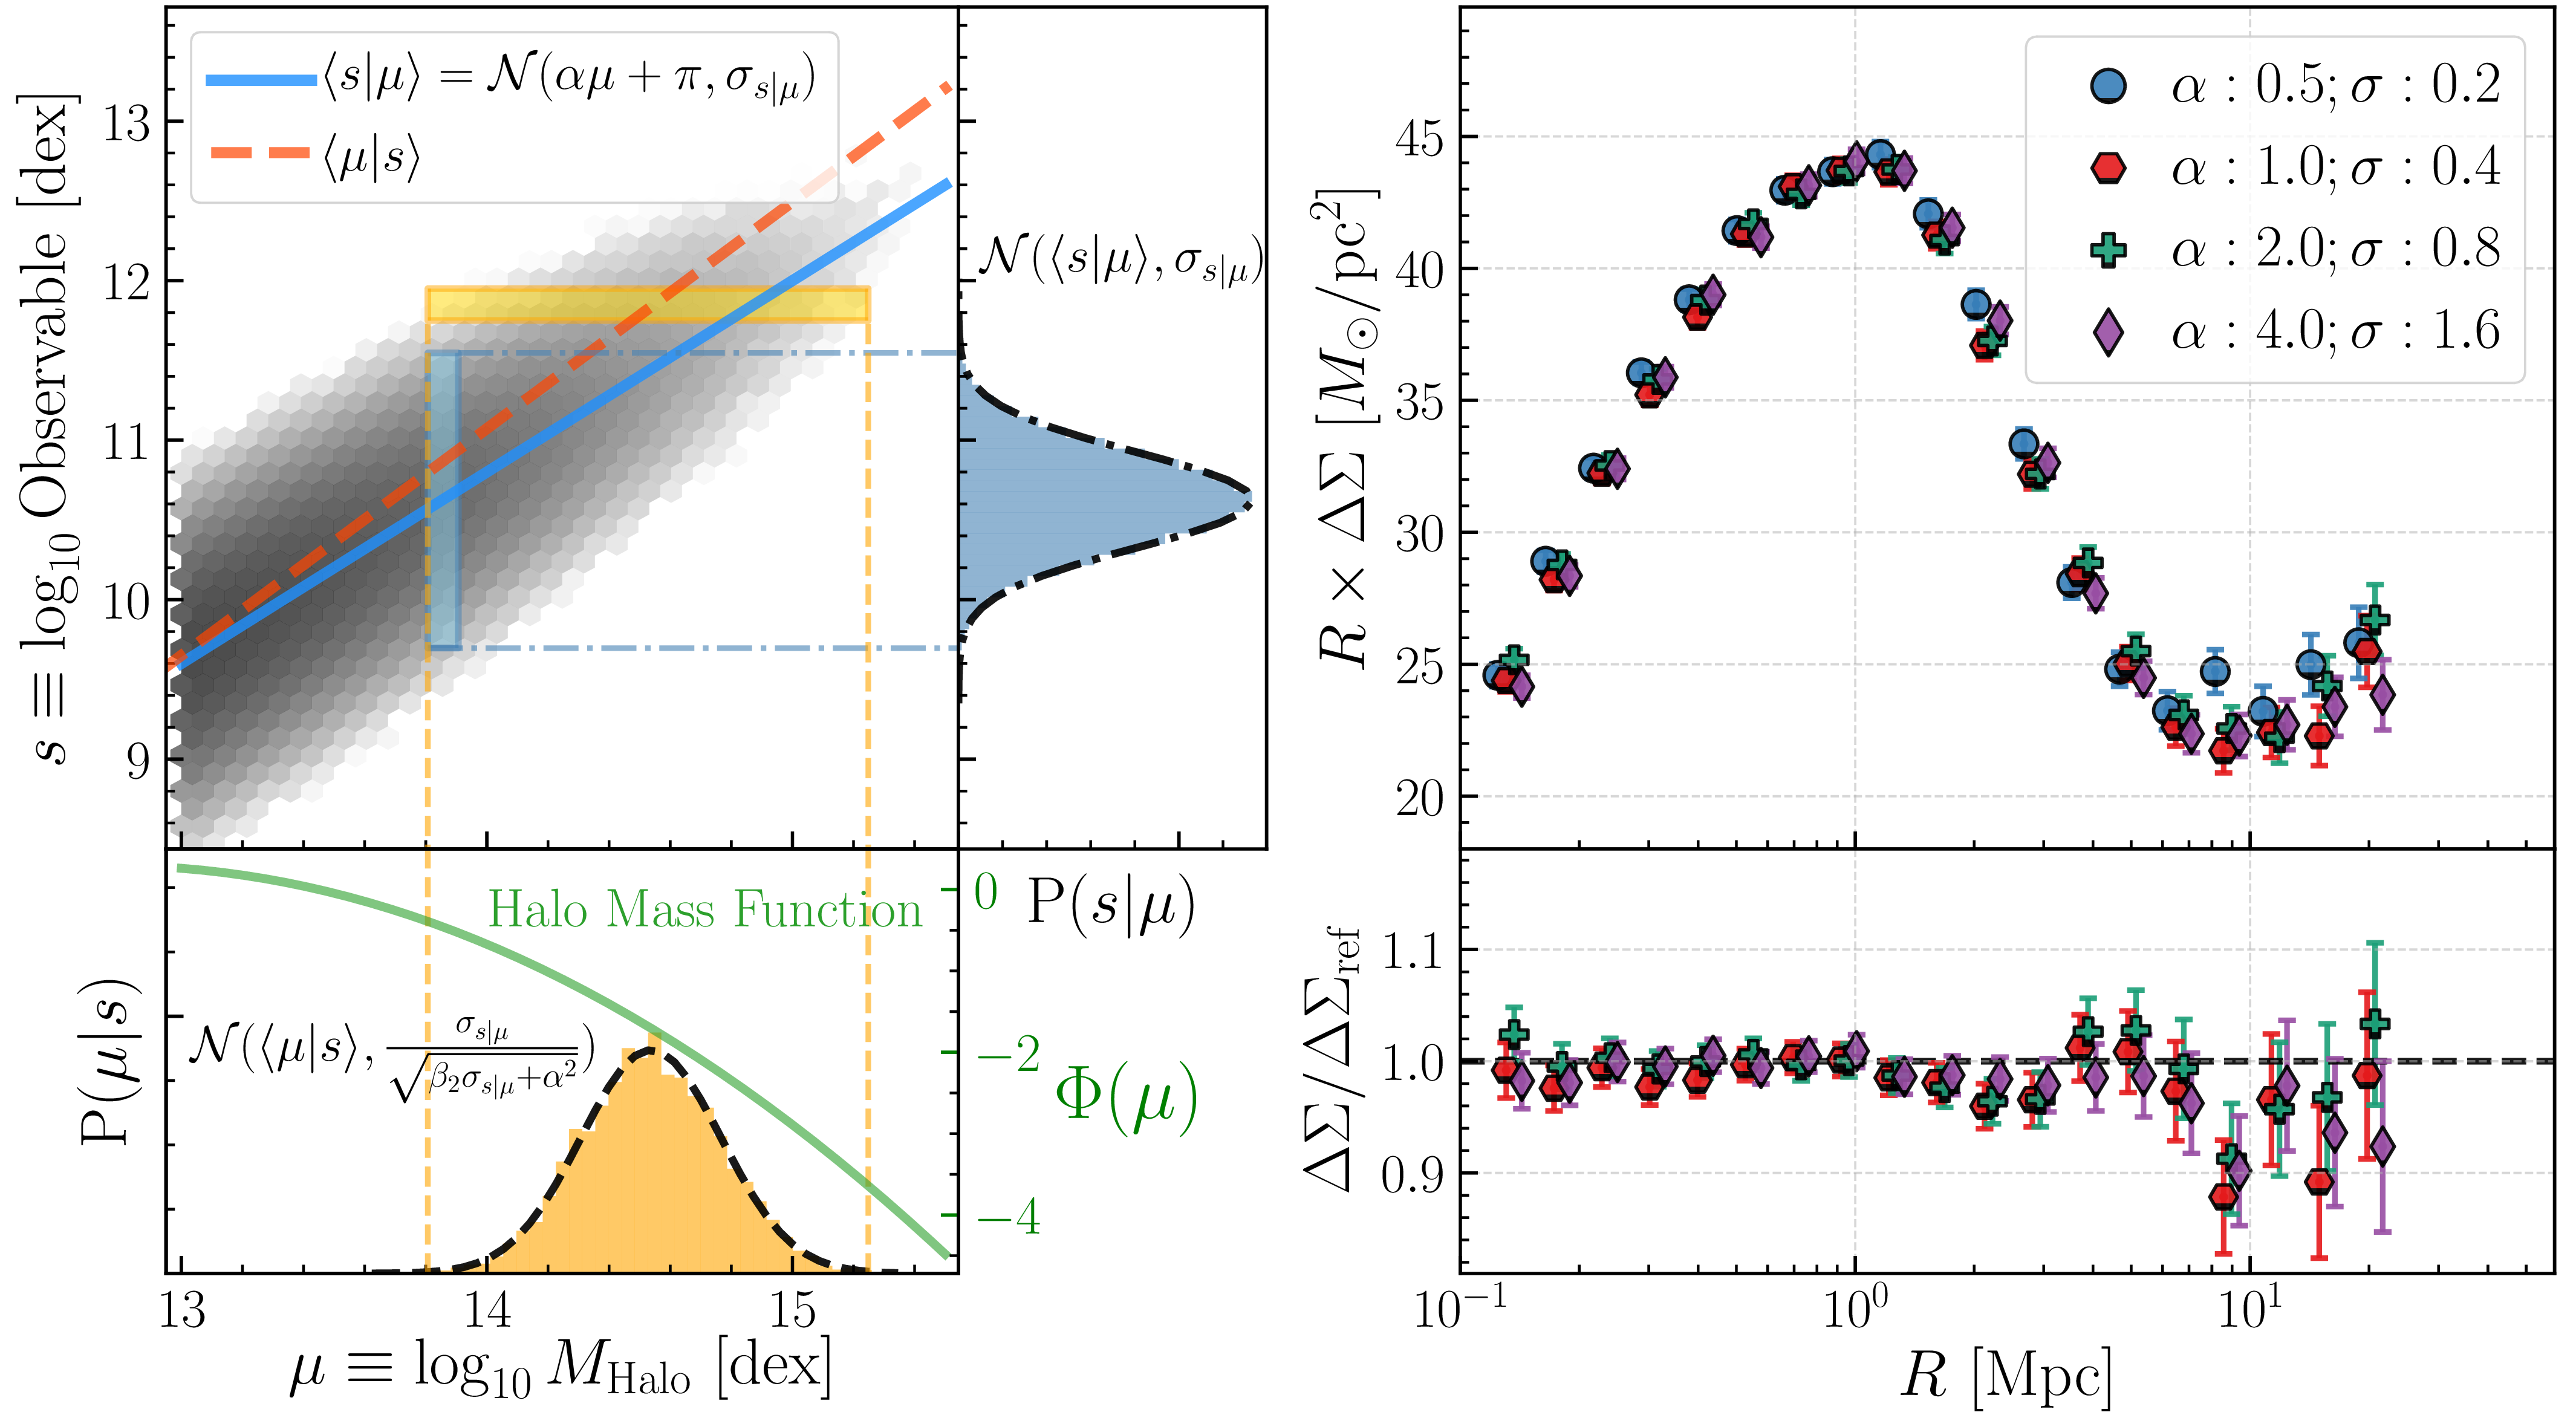
\includegraphics[width=\textwidth]{figure/theory.png}
  \caption{
     \textbf{Left}: The distribution of some observable, \obsSym{}, that is related to $\mu =
     \log(\Mhalo)$ by a linear relation with some scatter. By construction, $P(\obsSym | \mu)$
     (right panel, orange histogram) is normally distribution around $\langle \obsSym | \mu
     \rangle = \alpha \mu + \pi$ with a scatter of $\sigma_{\obsSym | \mu}$. The halo mass
     function (bottom panel, red line, right axis), is constructed using the best fit of a
     logarithmic quadratic (as in \ref{eq:quadratic_hmf}) to MDPL2. $P(\mu | \obsSym)$ (bottom
     panel, cyan histogram) is the distribution of $\mu$ given by a thin selection of \obsSym{}
     (main panel, cyan selection). This distribution of $\mu$ is well described by a normal
     distribution (green PDF) centered at the value given by \ref{eq:mean_of_mu} (cyan dashed
     line) with a scatter given by \ref{eq:scatter_of_mu} that depends on $\sigma_{\obsSym |
     \mu}$, the slope of the \obsSym - $\mu$ relation, $\alpha$, and the curvature of the mass
     function, $\beta_2$. The gap between $\langle \obsSym | \mu \rangle$ and $\langle \mu |
     \obsSym \rangle$ is smallest where the mass function is nearly flat (towards lower masses)
     while it becomes large at high masses where the steeper mass function leads to a large
     Eddington bias. \textbf{Right}: Observables with the same ratio $\alpha /
     \scatterObsSymMhalo$ have the same \scatterMhaloObsSym{} (see
     \ref{eq:ratio_is_what_matters}) and therefore the same \dsigma{} profile.
	}
    \label{fig:theory}
\end{figure*}
%% ---------------------------------------------------------------------------------------------- %%

%% ---------------------------------------------------------------------------------------------- %%
%% Figure: Demonstration of the mock catalog
%% ---------------------------------------------------------------------------------------------- %%
\begin{figure*}
  \centering
  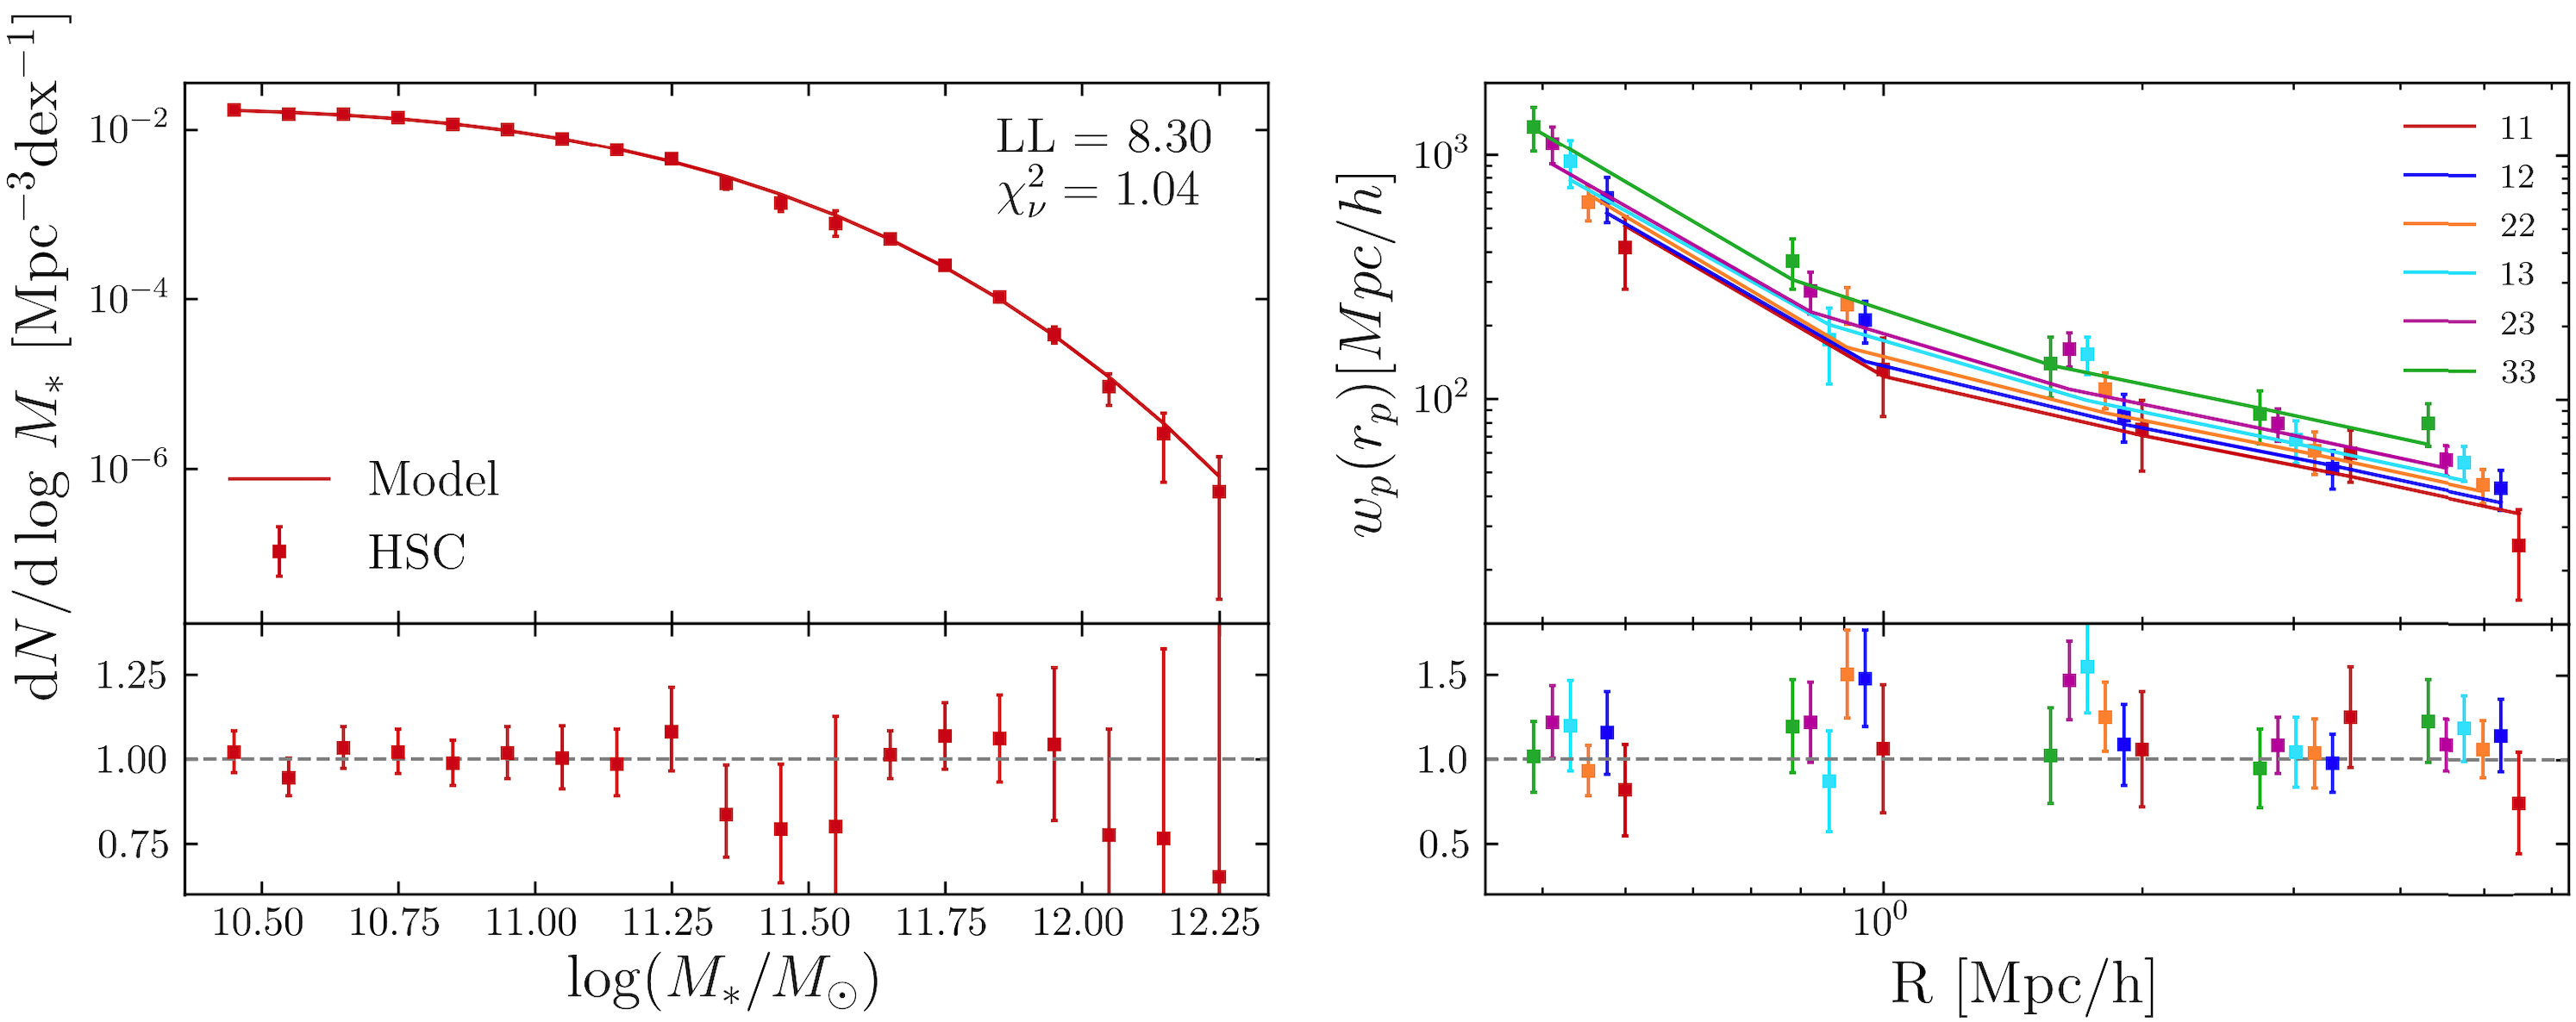
\includegraphics[width=\textwidth]{figure/mock_placeholder}
  \caption{\song{Placeholder} The best-fit mock matches both the SMF from HSC and \texttt{PRIMUS} 
    (left) as well as the clustering from HSC. The mass bins for the clustering are 
    [$11.5$, $11.55$, $11.7$, inf] and so e.g. ``11'' denotes the auto-correlation in the lowest 
    mass bin and ``13'' the cross correlation between objects in the lowest and highest mass bins.
    }
  \label{fig:best_mock}
\end{figure*}
%% ---------------------------------------------------------------------------------------------- %%


%% ---------------------------------------------------------------------------------------------- %%
%% Scaling relation and scatters
%% ---------------------------------------------------------------------------------------------- %%
\subsection{Simple Scaling Relation Model}
    \label{sec:scaling}

    We can model the effect on the \dsigma{} profile of various amounts of scatter between a
    generic observable, the log of which we denote as \obsSym{}, and the log of \mvir{}, denoted
    as $\mu$. We assume that the relationship between halo mass and the observable is modeled by
    a power law for the mean relation with log-normal scatter. This has been used for various
    observables, {\it e.g.,\addref{}} X-ray temperature \citet{Lieu2016}, K-band luminosity
    \citet{Ziparo2016}, and the details of the statistics of this relation are described in,
    amongst others, \citet{Evrard2014, Farahi2018}.

    The relationship between \obsSym{} and $\mu$ will depend on the distribution of $\mu$ - this
    is the halo mass function (HMF). To express the HMF over the full mass range, a functional
    form that follows a power law at low masses with an exponential decline at high masses is
    generally used \citep[\eg{}][]{Tinker2008}. However, as we are only interested in a narrow
    range at the high mass end, we can approximate it as an exponential decline with some
    curvature.

    \begin{equation}
        \hmf{} \equiv \frac{dn(\mu)}{d\mu{}}  = \exp \left(\beta_0 - \beta_1 \mu - \frac{\beta_2}{2} \mu^2 \right)
        \label{eq:quadratic_hmf}
    \end{equation}
    
    \noindent In practice, at the high mass end the mass function is decreasing ($\beta_1 > 0$)
    and steepening ($\beta_2 > 0$).
    
    We populate our simulation's halos with this generic observable,
    
    \begin{equation}
        \obsSym = \mathcal{N}(\slope \mu + \intercept,\ \scatterObsSymMhalo)
        \label{eq:lognormal_obs_given_mhalo}
    \end{equation}
    
    However, while \scatterObsSymMhalo{} is physically meaningful and the number most often
    quoted (\eg{} it is well known that $\scatterMstarx{cen} \sim 0.2$ dex) when comparing
    observables used to select halos, it is the scatter in \Mhalo{} at a fixed value for the
    observable, \scatterMhaloObsSym{}, that is important. We can compute the moments of $\mu |
    \obsSym$ as follows.
    
    We first note that the number of objects in a thin range of $\obsSym \in [\obsSym_1, \obsSym_2]$
    is given by,
    
    \begin{equation}
        N(\obsSym{}_1, \obsSym{}_2) \equiv \int_{\obsSym{}_1}^{\obsSym{}_2} \int_{-\infty}^{\infty} \hmf{} P(\obsSym{} | \mu) d\mu d\obsSym{}
    \end{equation}
    
    At fixed \obsSym{} we can therefore compute the expected $\mu$, and the scatter around it,

    \begin{equation}
    \begin{aligned}
        \langle \mu | \obsSym \rangle 
        &= \frac{1}{N(s_1, s_2)}
            \int_{-\infty}^{\infty} \hmf{} P(\obsSym{} | \mu) \mu d\mu \\
        &= \frac{\left( \frac{\obsSym- \intercept}{\slope} - \beta_1 \left(\frac{\scatterObsSymMhalo}{\slope}\right)^2 \right)}{ 1 + \beta_2 \left(\frac{\scatterObsSymMhalo}{\slope}\right)^2}
        \label{eq:mean_of_mu}
    \end{aligned}
    \end{equation}
    
    \noindent The three components of $\langle \mu | \obsSym \rangle$ are: 
    
    \begin{enumerate}
    	
        \item The relation between the observable and halo mass, $(\obsSym- \intercept) /
        \slope$.
        
        \item A shift due to the Eddington bias caused by the linear slope of the HMF, $-\beta_1
        (\scatterObsSymMhalo / \slope)^2$. In the case of $\beta_1 > 0$, this shift is to lower
        $\mu$ as there are more low $\mu$ objects that can be up-scattered into the selection
        than can be down-scattered.
        
        \item A second shift due to excess Eddington bias caused by the curvature of the HMF, $(1
        + \beta_2 (\frac{\scatterObsSymMhalo}{\slope})^2)^{-1}$. Again, $\beta_2 > 0$ results in
        more low $\mu$ objects and thus a shift to lower $\mu$.
    	
    \end{enumerate}
    
    Similarly, the scatter in $\mu$ at fixed $\obsSym$,

    \begin{equation}
    \begin{aligned}
        \scatterMhaloObsSym{} 
        &= \frac{1}{N(s_1, s_2)}
            \int_{-\infty}^{\infty} \hmf{} P(\obsSym{} | \mu) ( \mu  - \langle \mu \rangle )^2 d\mu \\
    	&= \frac{\scatterObsSymMhalo}{\sqrt{\beta_2 \scatterObsSymMhalo^2 + \slope^2}}
        \label{eq:scatter_of_mu}
    \end{aligned}
    \end{equation}
    
    \noindent which, in the case of a power law mass function, reduces to the commonly seen
    $\scatterObsSymMhalo / \slope$. The positive $\beta_2$ of the HMF decreases this scatter.
    Finally, higher moments show that $P(\mu | s)$ is Gaussian, as there is no skew or excess
    kurtosis.
    
    These results are summarized in the left panel of Figure \ref{fig:theory} where we simulate
    the HMF and the theoretical observable \obsSym{}. We show that the resulting distributions
    are consistent with the results shown here.
    
    This theoretical understanding of the moments on $\mu | \obsSym$ shows us what range of slope
    and scatter we need to generate \dsigma{} profiles for. While naively this is a 2 dimensional
    problem, \ref{eq:scatter_of_mu} shows that it can be reduced to a single dimension where
    \scatterMhaloObsSym{} is a function of the ratio between slope and scatter. This is obvious
    in the case where $\beta_2 = 0$ but still true in the curved case,

    \begin{equation}
        \scatterMhaloObsSym{} 
        	= \frac{\scatterObsSymMhalo}{\sqrt{\beta_2 \scatterObsSymMhalo^2 + \slope^2}}
            = \left(\beta_2 + (\frac{\slope}{\scatterObsSymMhalo})^2\right)^{-1/2}
        \label{eq:ratio_is_what_matters}
    \end{equation}
    
    This is shown in the right panel of Figure \ref{fig:theory}. For a variety of observables
    with a range of $\alpha$ and \scatterObsSymMhalo{}, but with the same ratio $\alpha /
    \scatterObsSymMhalo$, and therefore the same \scatterMhaloObsSym{}, the \dsigma{} is
    identical. Therefore, in order to compare the \dsigma{} from a range of observables with
    different slope/scatter compared to have mass, we can fix one parameter ($\alpha = 1$) and
    vary the other ($\scatterObsSymMhalo$) to achieve the goal \scatterMhaloObsSym{} in the
    number density bins discussed in \ref{sec:topn_intro}. In practice, rather than predict the
    \scatterMhaloObsSym{} using \ref{eq:scatter_of_mu} (which requires fitting for $\beta_2$ at
    that point in the HMF), we instead binary search for the desired \scatterMhaloObsSym{} by
    iteratively choosing a \scatterObsSymMhalo{} to populate the halos with, and then fitting a
    linear $\mu | \obsSym$ to the relation in the given halo mass bin. The results of this
    process are shown in \ref{fig:mdpl2} where we predict \dsigma{} profiles as a function of
    \scatterMhaloObsSym{} for each of the number density bins. We will compare these theoretical
    predicts to the observables to estimate their \scatterMhaloObsSym{}.

%% ---------------------------------------------------------------------------------------------- %%
%% Model used in comparison
%% ---------------------------------------------------------------------------------------------- %%
\subsection{Model Calibrated to Match HSC}
    \label{sec:halo_model}

    \todo{Placeholder: Updates needed}
    
    While the simple scaling relation model presented above is useful to predict the effects of
    scatter between an observable and halo mass on the lensing signal, a more detailed model of
    the galaxy halo connection is needed to compare with specific model of M100. To make
    comparisons the HSC observations and theory, we need to populate the simulation with
    realistic galaxies. This process will be described in more detail in (Bradshaw et. al. in
    prep.)) but we summarize it here.
    
    To do this, we use the 1 Gpc MultiDark-Planck simulation. We populate galaxies using an
    abundance matching model based on the \citet{Lehmann2017} $\alpha$ model. This model
    marginalizes over the choice of the halo property to abundance match on. In this analysis, we
    use the mock that best fits the HSC high mass clustering, the auto- and cross-correlation of
    $\omega_p$ in bins of stellar mass [$11.5$, $11.55$, $11.7$, inf], and the combination of the
    SMF from HSC and \texttt{PRIMUS}. We use the HSC SMF in the mass regime that is complete ($>
    11.5$) and \texttt{PRIMUS} for lower masses ($10.5 - 11.5$).
    
    The best-fit mock is able to reproduce the mass function and clustering statistics of HSC as
    shown in \ref{fig:best_mock}.

%% ---------------------------------------------------------------------------------------------- %%
%% Figure: Definition of richness and number density bins.
%% ---------------------------------------------------------------------------------------------- %%
  \begin{figure*}
      \centering 
      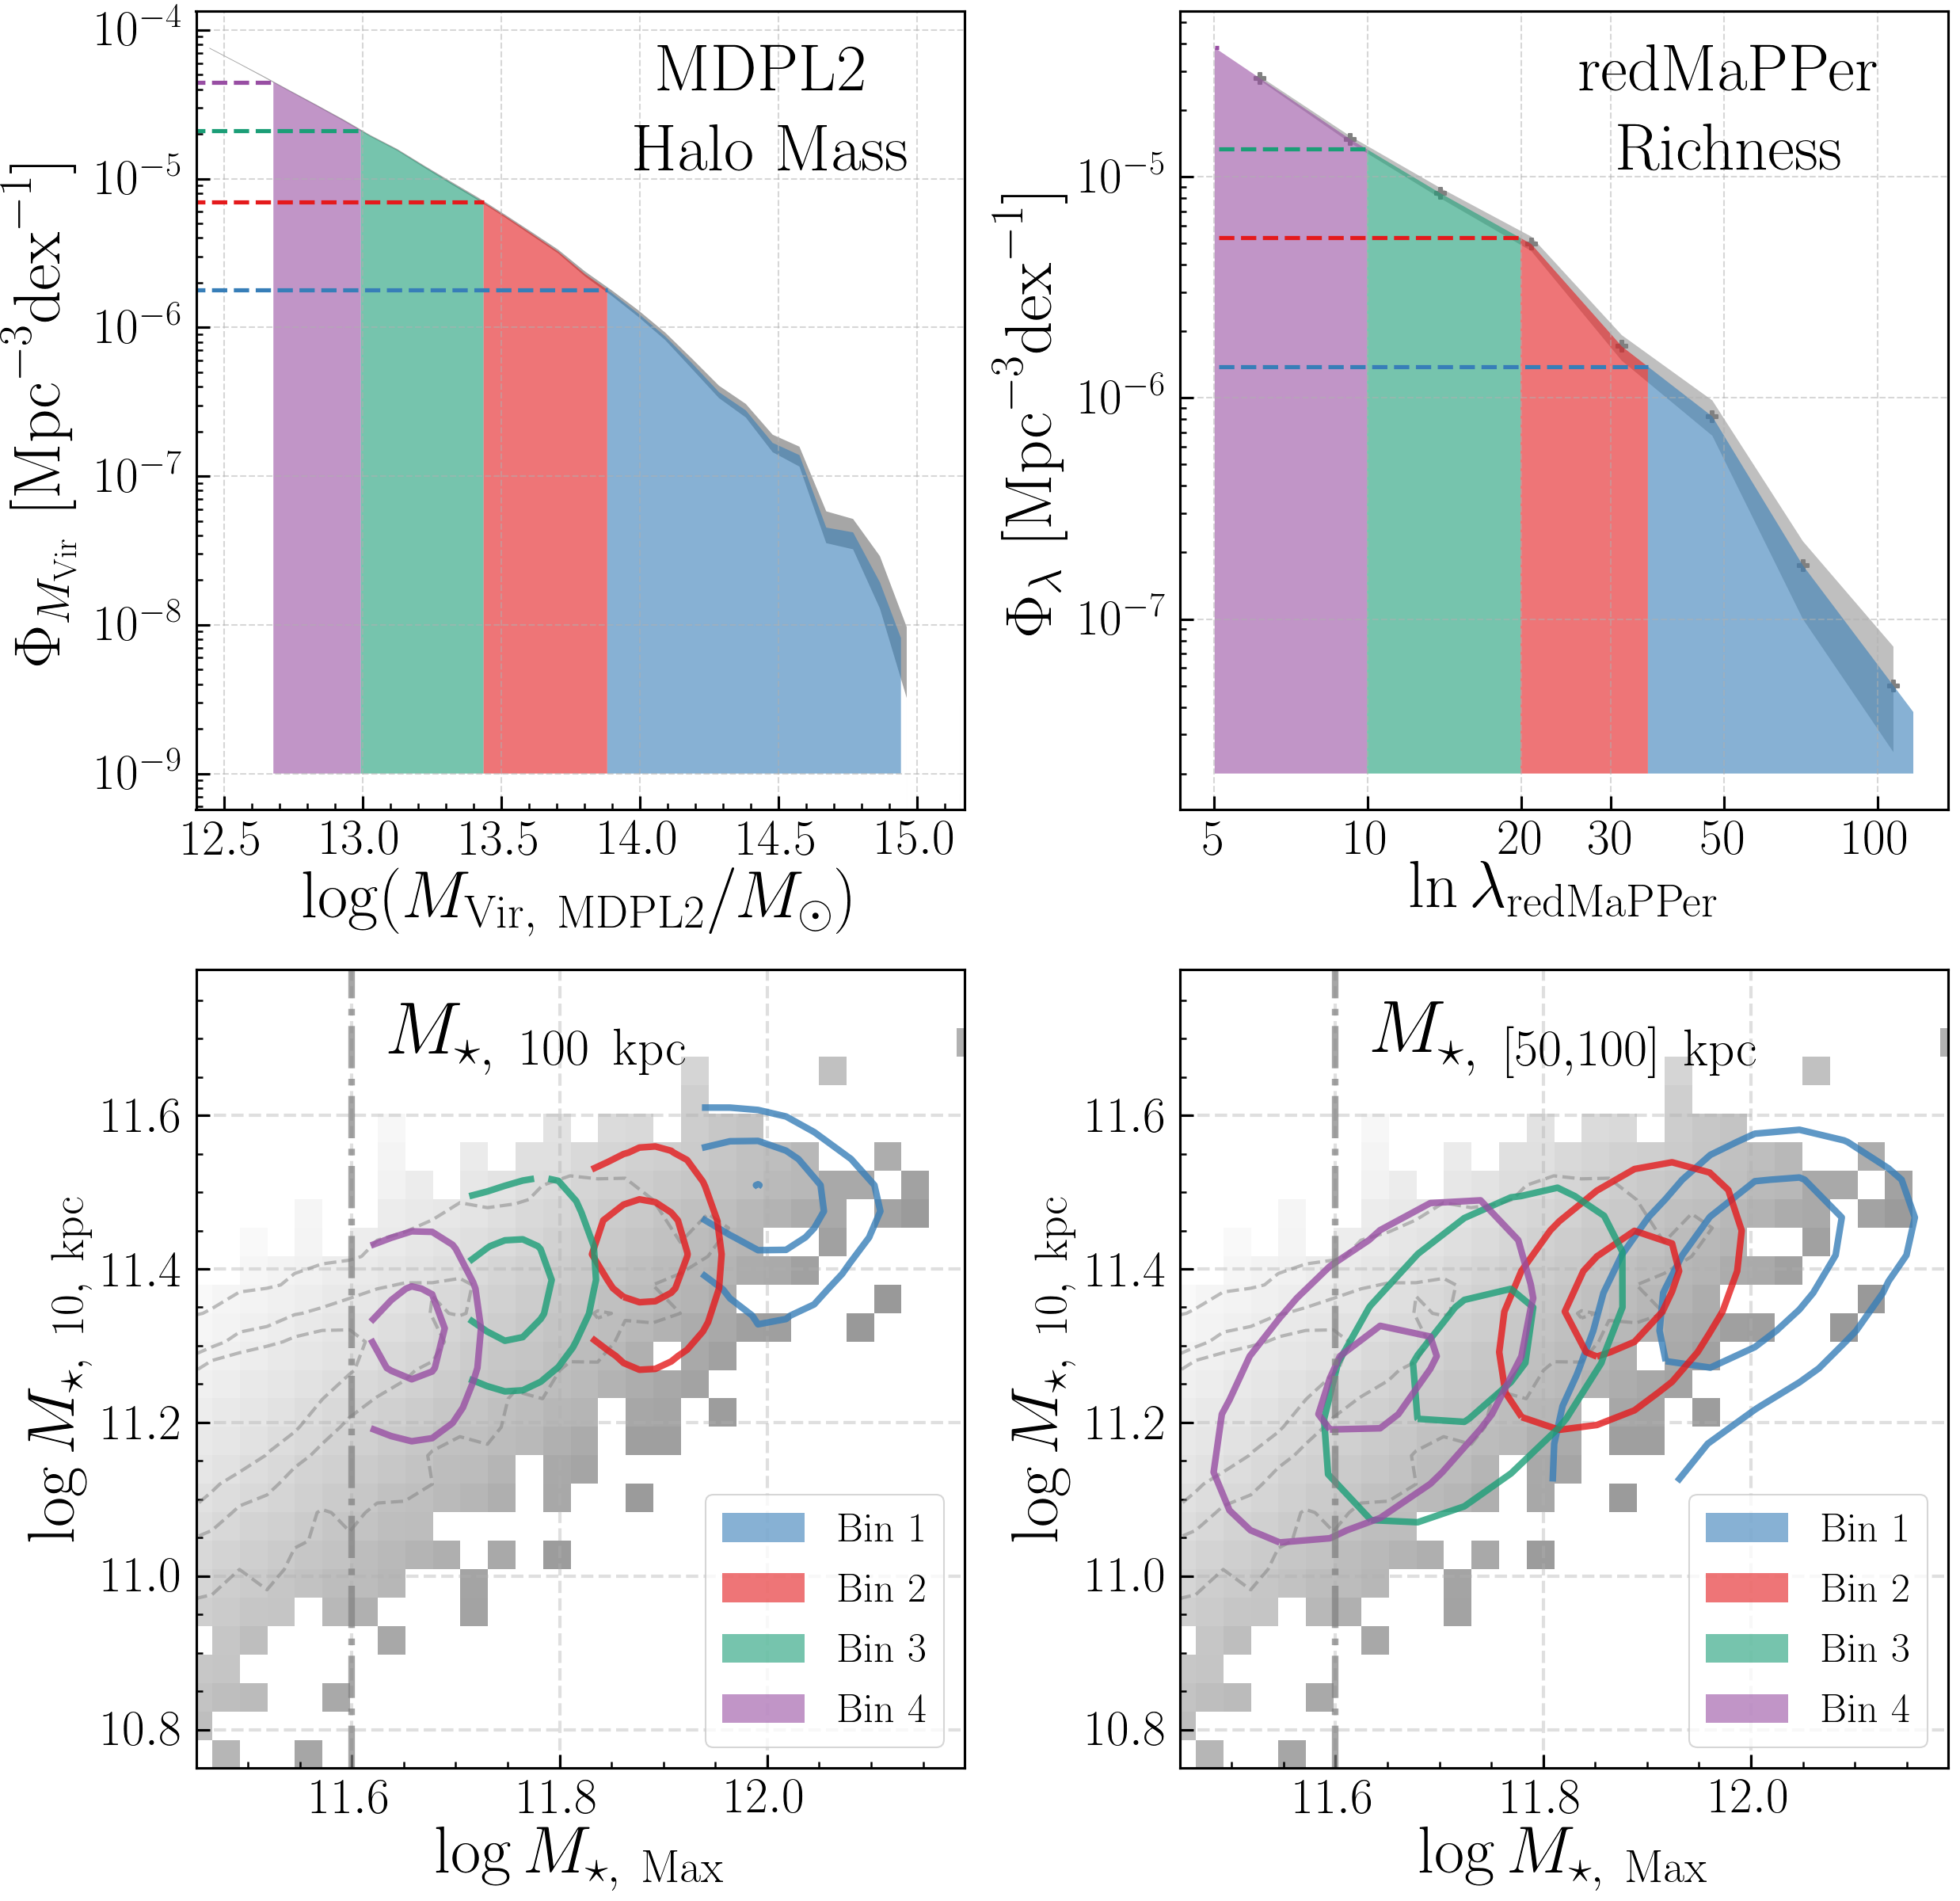
\includegraphics[width=\textwidth]{figure/topn_bins}
      \caption{The four bins used for our "top-N" tests. The left panel displays bins in
          $\lambda$, the middle panel displays bins in \mmax{}, and the right panel displays bins
          in $M_{\rm vir,\ ASAP}$. Bins are defined at fixed number density. \alexie{Add a table
          for each of the quantities with the edges of the bin and the mean bin. This can be two
          panels. The phi one on the left and the two parameter cut on the right to highlight why
          samples can be different}}
      \label{fig:density_bins}
  \end{figure*}
%% ---------------------------------------------------------------------------------------------- %%

%% ---------------------------------------------------------------------------------------------- %%
%% Introducing the TopN test and define the number density
%% ---------------------------------------------------------------------------------------------- %%
\section{``Top N'' Tests}
    \label{sec:topn_intro}   

    \plan{Placeholder: A very rough outline}

    \begin{itemize}
        
        \item \plan{Basic philosophy}: Comparison of \dsigma{} profiles of massive halos 
            identified by different methods within the same volume number density threshold.
        
        \item \plan{Binning}: four bins based on the richness values of HSC \redm{} cluster 
            catalog. Bin 1 \& 2 correponds to the \mvir{} range of galaxy clusters; 
            Bin 3 \& 4 reach into the massive galaxy group regime.
        
        \item \plan{Comparison with model \dsigma{} profiles and the estimate of \sigmh{}.}

    \end{itemize}

    \todo{Points worth mentioning, randomly organized.}
    \plan{Mention that the \mstar{} sample misses $\sim 10$\% of galaxies due to failed 1-D
        profile extraction. Visual examination of the failed ones and their \mcmodel{}
        suggest that the \mstar{} distribution of those cases should not be that different 
        from the overal SMF. Some of these cases are on-going mergers or double-core
        BCGs. We do not correct for the difference in the effective volume caused by this.
        Verying the number density threshold by $\sim 10$\% accordingly does not change any
        key result.}

    \plan{We should note that there are plenty of previous works that carefully model the \dsigma{}
        profiles of massive clusters to extract information including the average \mvir{} (e.g.,
        \addref{}).
        Both \redm{} and \camira{} cluster finders have their \mvir{}-richness relations calibrated 
        using sophisticated forward-modeling of cluster \dsigma{} profiles (e.g., 
        \citealt{Murata2018, Murata2019}, \addref{}). 
        These models often include different components such as the so-called 1-halo and 2-halo
        terms along with the contribution of off-center clusters.}

%% ---------------------------------------------------------------------------------------------- %%
%% Figure: DSigma profiles from MDPL2 and the impacts of scatter on DSigma profile and 
%%         halo mass distribution
%% ---------------------------------------------------------------------------------------------- %%
  \begin{figure*}
      \centering 
      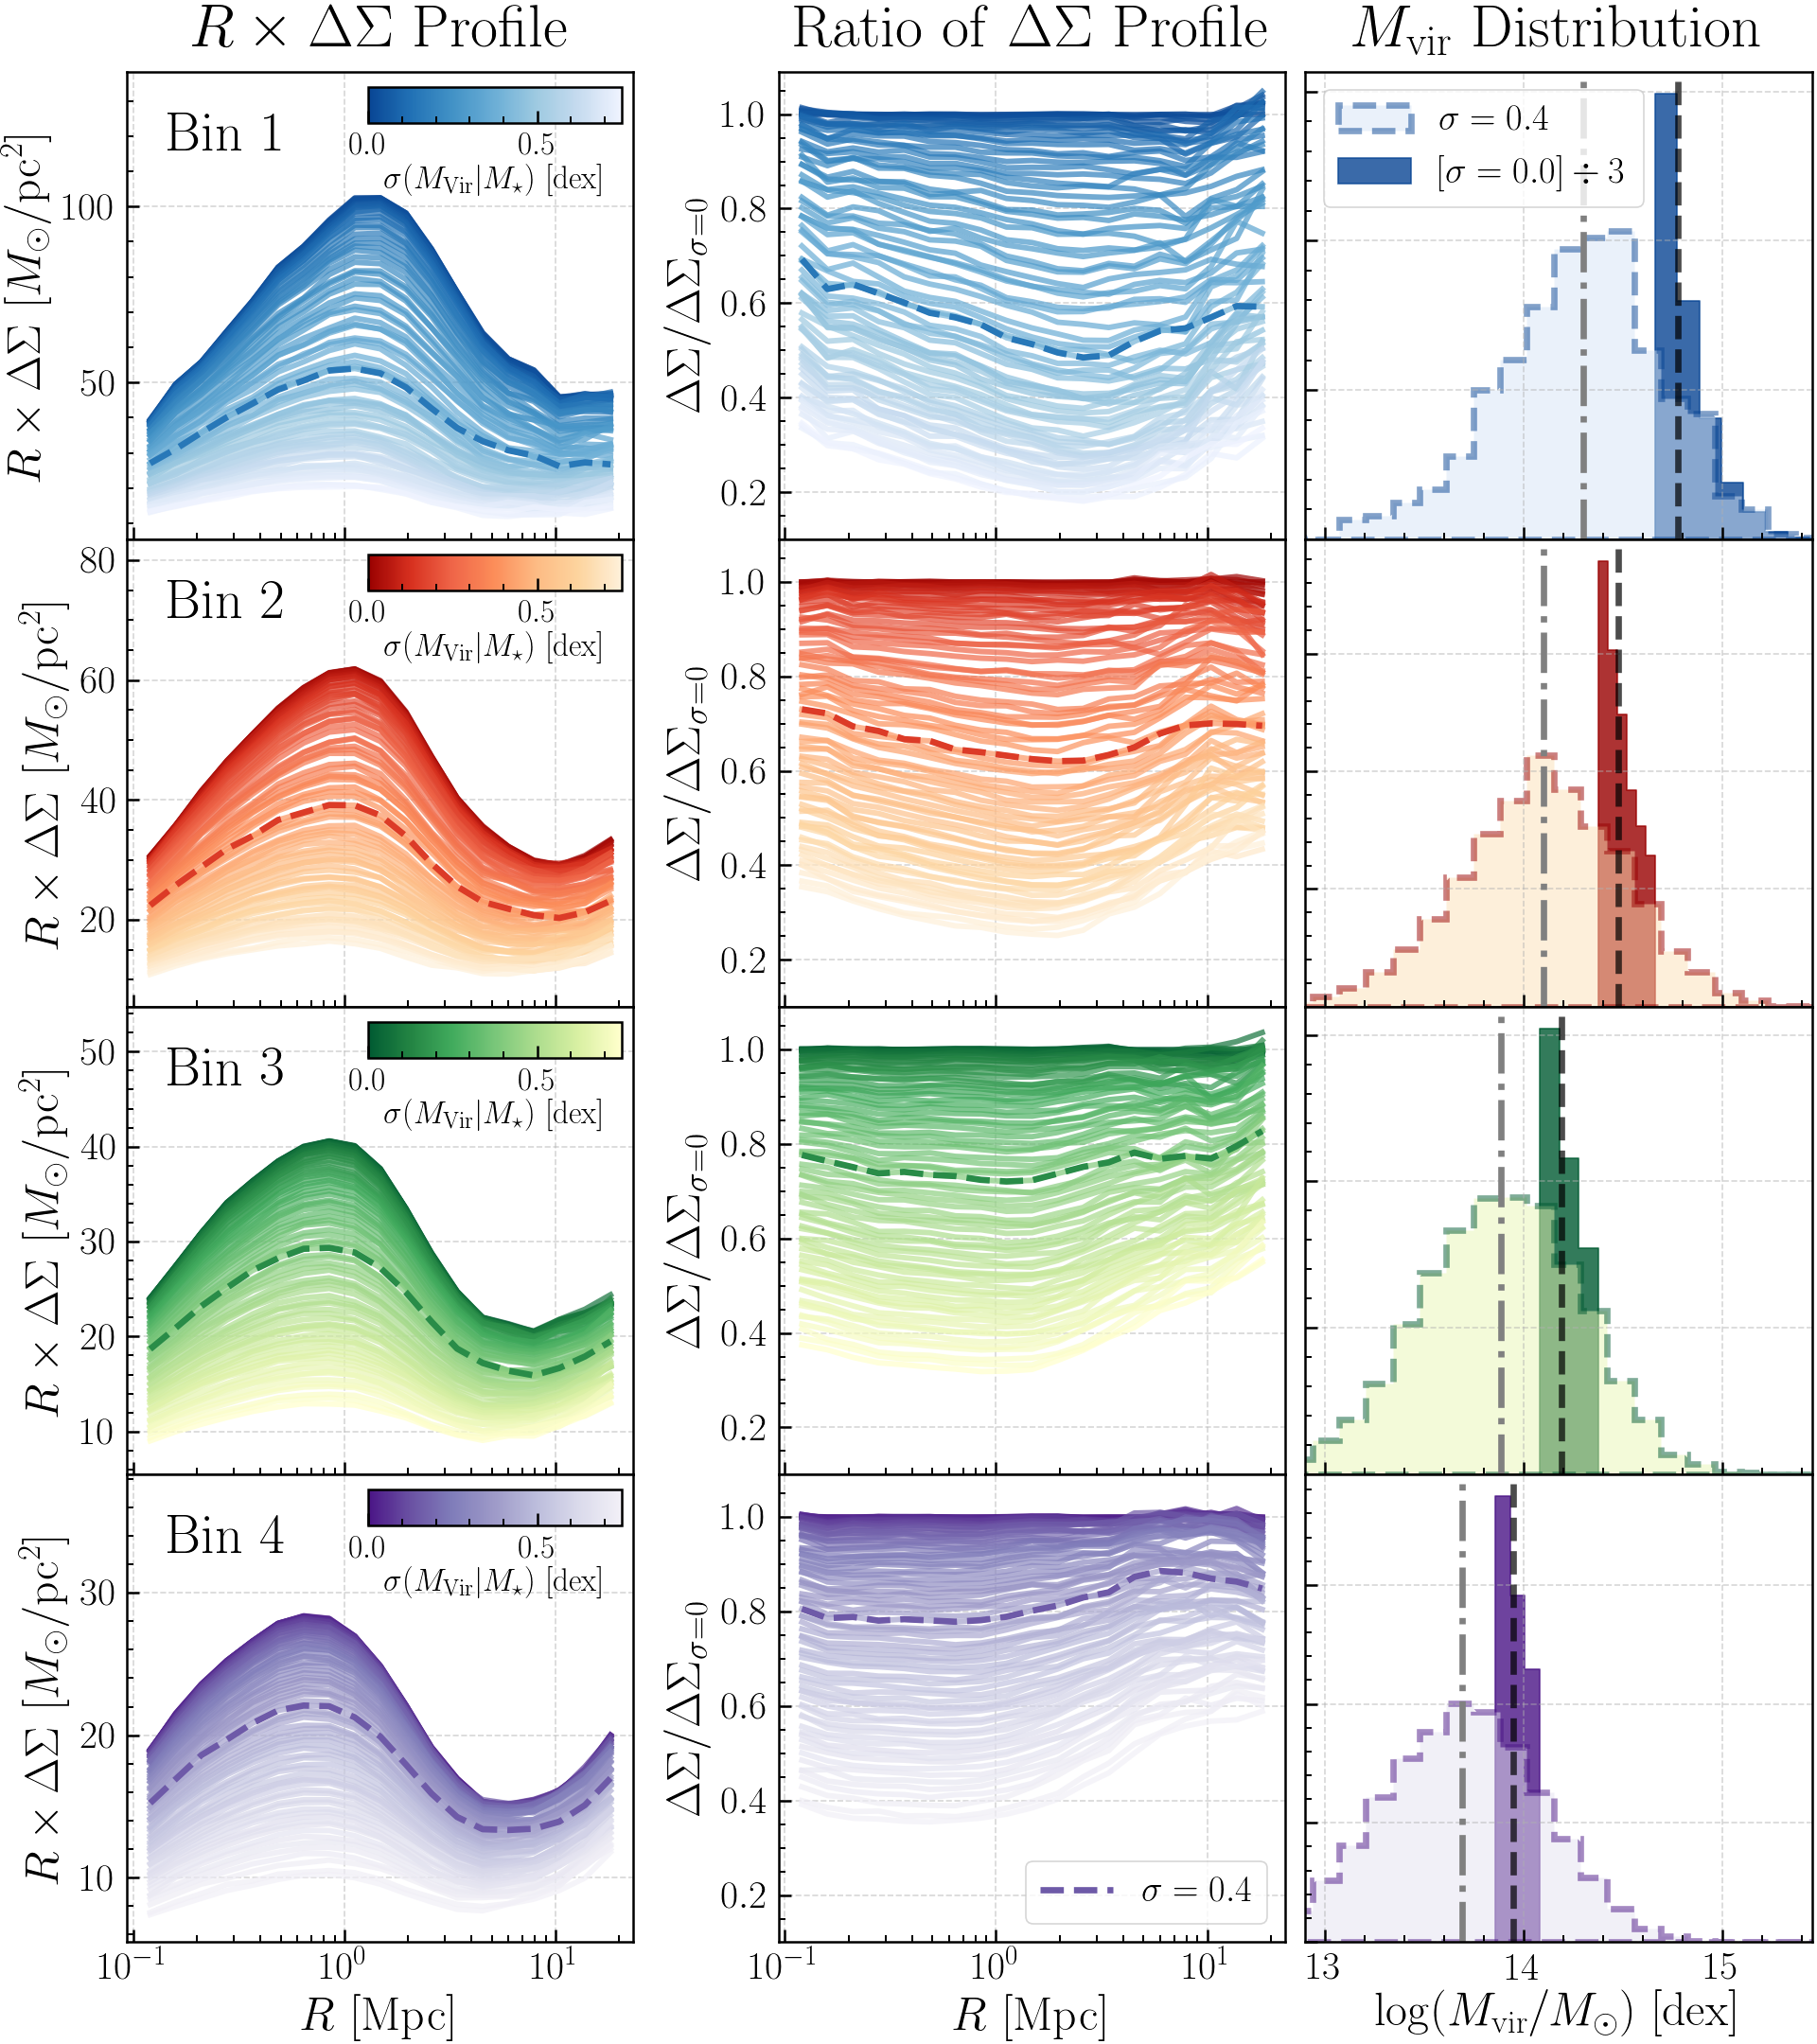
\includegraphics[width=\textwidth]{figure/topn_mdpl2_dsigma}
      \caption{Impact of scatter in the mass-observable relation on $\Delta\Sigma$. Left: the
        $\Delta\Sigma$ profiles for $0<\sigma_{Mvir|obs}<2$. Middle: ratio of $\Delta\Sigma$ with
        non zero scatter to $\Delta\Sigma$ when $0<\sigma_{Mvir|obs}=0$. Right: halo mass
        histograms for bin 1 ($\overline(n)=x$) and bin 2 ($\overline(n)=x$).} \label{fig:mdpl2}
  \end{figure*}
%% ---------------------------------------------------------------------------------------------- %%

%% ---------------------------------------------------------------------------------------------- %%
%% Table.1 
%% ---------------------------------------------------------------------------------------------- %%
%\clearpage
\begin{table*}
\resizebox{0.7\textwidth}{!}{%
\small
\begin{tabular}{|c|cccc|}
\hline
\rowcolor[HTML]{d8dcd6} Property   & Bin 1   & Bin 2   & Bin 3  & Bin 4 \\ \hhline{|=====|}

$N_{\rm Sample}$     &   50  &  197  &  662  &  1165  \\  

$\log_{10} M_{\rm vir,\ \rm MDPL2}$  & [14.66, 15.55] & [14.38, 14.66) & [14.08, 14.38) & [13.86, 14.08) \\

$n(>M_{\rm vir})$  & $5.11\times 10^{-7}$ & $2.52\times 10^{-6}$ & $9.29\times 10^{-6}$ & $2.12\times 10^{-5}$ \\ \hhline{|=====|}

\multirow{2}{*}{$\lambda_{\rm redMaPPer}$}  &  [35, 120] &  [20, 35)  & [10, 20) &  [6, 10)  \\
& \sigmvir{}$=0.27\pm0.02$ & $0.38\pm0.02$ & $0.39\pm0.02$ & $0.58\pm0.02$ \\ \hline
                                            
\multirow{2}{*}{$N_{\rm CAMIRA}$}  &  [35, 75) & [21, 35) & [12, 21) &  \\
& \sigmvir{}$=0.30\pm0.03$ & $0.36\pm0.01$ & $0.50\pm0.02$ & {} \\ \hhline{|=====|}

\multirow{2}{*}{$\log_{10} M_{\star, \rm CModel}$}   & [11.88, 12.19] & [11.77, 11.88) & [11.67, 11.77) & [11.60, 11.67) \\ 
& \sigmvir{}$=0.60\pm0.04$ & $0.64\pm0.04$ & $0.87\pm0.06$ & $0.82\pm0.03$ \\ \hline

\multirow{2}{*}{$\log_{10} M_{\star, 30\ \rm kpc}$} & [11.77, 12.00] & [11.69, 11.77) & [11.61, 11.70) & [11.53, 11.61) \\ 
& \sigmvir{}$=0.52\pm0.04$ & $0.57\pm0.03$ & $0.61\pm0.03$ & $0.61\pm0.02$ \\ \hline

\multirow{2}{*}{$\log_{10} M_{\star, 50\ \rm kpc}$} & [11.86, 12.10] & [11.76, 11.86) & [11.66, 11.76) & [11.58, 11.66) \\ 
& \sigmvir{}$=0.46\pm0.04$ & $0.53\pm0.03$ & $0.59\pm0.02$ & $0.61\pm0.02$ \\ \hline

\multirow{2}{*}{$\log_{10} M_{\star, 100\ \rm kpc}$} & [11.93, 12.18] & [11.83, 11.93) & [11.71, 11.83) & [11.63, 11.71) \\ 
& \sigmvir{}$=0.38\pm0.02$ & $0.51\pm0.02$ & $0.56\pm0.02$ & $0.60\pm0.02$ \\ \hline

\multirow{2}{*}{$\log_{10} M_{\star, 150\ \rm kpc}$} & [11.96, 12.21] & [11.85, 11.96) & [11.73, 11.85) & [11.64, 11.73)  \\ 
& \sigmvir{}$=0.37\pm0.03$ & $0.47\pm0.03$ & $0.56\pm0.02$ & $0.57\pm0.03$ \\ \hhline{|=====|}

\multirow{2}{*}{$\log_{10} M_{\star, [50, 100]}$} & [11.20, 11.60] & [11.00, 11.20) & [10.80, 11.00) & [10.63, 11.00)  \\ 
& \sigmvir{}$=0.36\pm0.02$ & $0.43\pm0.02$ & $0.44\pm0.02$ & $0.48\pm0.02$ \\ \hline

\multirow{2}{*}{$\log_{10} M_{\rm Vir,\ ASAP}$} & [14.45, 15.28] & [14.09, 14.45) & [13.80, 14.11) & [13.60, 13.80)  \\ 
& \sigmvir{}$=0.38\pm0.03$ & $0.44\pm0.02$ & $0.48\pm0.02$ & $0.56\pm0.02$ \\ \hline

\end{tabular}%
}
\caption{
	Summary of results from the \topn{} test results in four number density bins. 
	The first three rows summarize the basic properties of each bin.
	$N_{\rm sample}$ is the number of HSC galaxies in each bin. 
	$\log_{10}M_{\rm vir, MDPL2}$ shows the corresponding halo mass range in this number density bin
	based on the \mdpl2{} simulation. 
	This is the \mvir{} range for an ideal (zero scatter) \topn{} selection.
	$n(>M_{\rm Vir})$ is the volume number density of halos above the lower-\mvir{} threshold.
	Subsequent rows contain the key results for different halo mass proxies. 
	The first row shows the range of the observed properties in the four bins.  The second row shows
	the best--fit scatter of \mvir{} at fixed observable ($\sigma_{\mathcal{M}|\mathcal{O}}$) of
	\mvir{} in each bin along with its uncertainty.
	For a complete summary table of all the properties we tested, please see this \texttt{Jupyter} notebook \href{https://github.com/dr-guangtou/jianbing/blob/master/notebooks/topn_result_summary.ipynb}{\faGithub} 
	}
\label{tab:summary}
\end{table*}
%\clearpage
%% ---------------------------------------------------------------------------------------------- %%

%% ---------------------------------------------------------------------------------------------- %%
%% Main Results
%% ---------------------------------------------------------------------------------------------- %%
\section{Results}
    \label{sec:result}

    Now we summarize the main results of this work. 
    We first qualitatively evaluate the impact of satellite galaxies on using \mstar{} of massive
    galaxies as promising \mvir{} proxy (Sec \ref{sec:satellite}).
    Then we show the key findings from the from the ``Top N'' tests and compare the performance
    of different \mvir{} tracers (Sec \ref{sec:topn_results}).
    We will highlight the behaviors of \mcmodel{} (Sec \ref{sec:cmodel}) and \mstar{} 
    of the outskirt of massive galaxies such as \menve{50}{100} (Sec \ref{sec:moutskirt}) 
    before we summarize the overall trends of \sighalo{} with volume number density for different
    \mvir{} proxies (Sec \ref{sec:trend}).
    Finally, we will compare the \dsigma{} profiles of the \mstar{}- and richness-selected 
    massive halos and explore their differences at the same number density bins
    (Sec \ref{sec:mstar_vs_richness}).

    Before we dive in, we want to remind the readers that
    1) All the \sighalo{} values mentioned in this work are the scatter of \mvir{} \emph{within each
    number density bin}. We do not attempt to calibrate or forward-model the \mvir{}-observable 
    relation, therefore we can not predict the scatter of \mvir{} \emph{at any given value of 
    the observable}.
    2) All the \sighalo{} values should be treated in a relative sense. We adopt strong
    assumptions when we ``model'' the \dsigma{} profile such as $\log$-linear relation with 
    constant and symmetric scatter, no consideration of mis-centering effect or projection effect.
    It is possible that the \sighalo{} value deviates from the ``true'' answer. 
    However, the \sighalo{} values for different observables in the same bin should provide 
    insights about the underlying \mvir{} distributions, and help us evaluate their pros and cons 
    when using them as \mvir{} proxy.

%% ---------------------------------------------------------------------------------------------- %%
%% Figure: Impact of satellites on the M100kpc selected DSigma profiles
%% ---------------------------------------------------------------------------------------------- %%
  \begin{figure}
      \centering 
      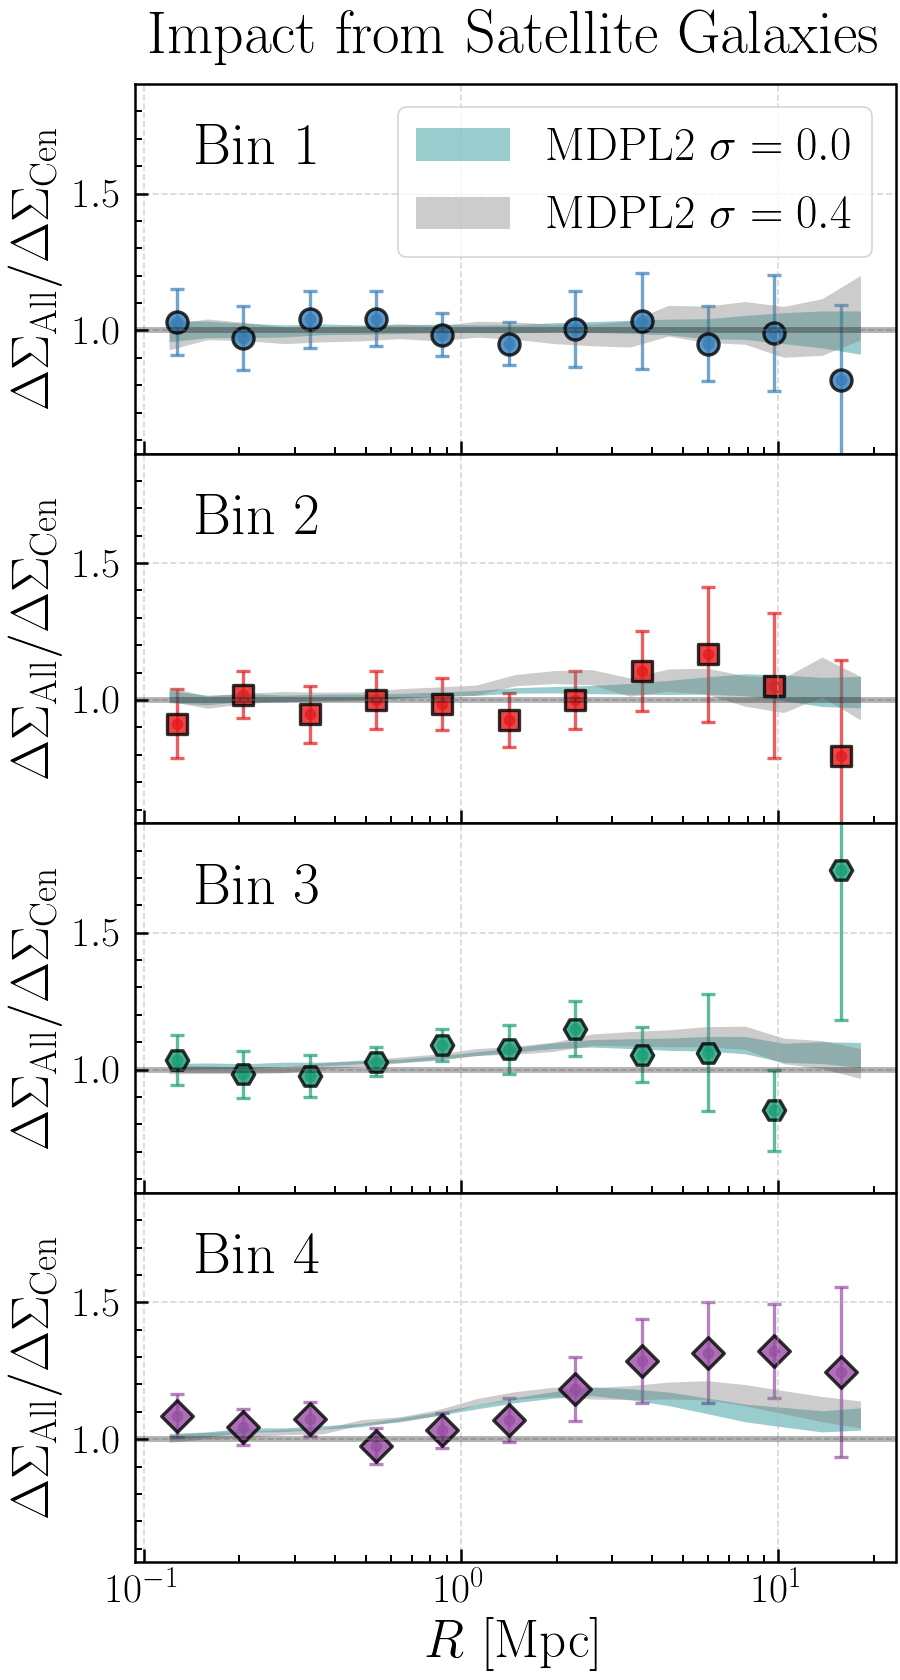
\includegraphics[width=0.49\textwidth]{figure/dsigma_sat_ratio}
      \caption{
          \todo{Impact of satellites on the M100kpc selected \dsigma{} profiles}
          }
      \label{fig:satellite}
  \end{figure}
%% ---------------------------------------------------------------------------------------------- %%

%% ---------------------------------------------------------------------------------------------- %%
%% Impact of satellite galaxies 
%% ---------------------------------------------------------------------------------------------- %%
\subsection{Impact of Satellites}
    \label{sec:satellite}

    \plan{A detailed outline}

    \begin{itemize}
        
        \item To fully realize the potential of using \mstar{} of a massive galaxy as \mhalo{}
            proxy, we must first deal with one crucial systematic issue which is the impact
            from satellite galaxies.
            Many previous works suggest a low satellite fraction at \logms{}$>$11.5, but 
            massive satellite galaxies still make up $\sim 5$-10\% of our sample.
            Moreover, satellite fraction significantly increases with decreasing \mstar{},
            presenting further challenges to apply \mstar{} as halo mass proxy.
        
        \item \plan{Briefly explain the impact of satellite galaxies on the \dsigma{} profile.}
            Their \dsigma{} profiles will show significant contribution from the host halo 
            in the second-halo term regime (e.g. \addref{}, Li et a. 2014).
        
        \item Here, we qualitatively investigate the impact of satellite galaxies. 
            On the simulation side, we directly compare the \dsigma{} profiles of just central 
            mock galaxies with the ones using all galaxies in each bin.
            We perform this comparison for model with \sigmh{}$=0.0$ and 0.4.
        
        \item For our HSC sample, we adopt a very simple strategy to identify potential 
            satellite galaxies. 
            Starting from the most massive galaxies defined by \mmax{} in our sample, 
            we iteratively find nearby massive galaxies in a cylinder-like region with 
            a 2.0 physical Mpc radius in projection and a 30 comoving Mpc length in the 
            line-of-sight (LOS) direction. 
            To calculate the LOS distance, we use the best available redshift and ignore 
            its uncertainty.
            \plan{The satellite fraction in each bin is [XX, XX, XX, XX]}.
            
        \item Such approach is certainly over-simplified as 1) the more massive galaxy 
            measured in our analysis is not necessarily the true central galaxy.
            2) The choice of cylinder size and the photo-$z$ uncertainty could mistakenly 
            remove central galaxy from the sample or leave satellites in.
            But it is sufficient to demonstrate the effect of satellite galaxies.
            We also explore several different choices of the cylinder size to make sure
            our result is robust.
            Replacing \mmax{} with other larger aperture \mstar{} when identifying satellites 
            will also not change the result.
        
        \item Figure \ref{fig:satellite} summarizes the result of the test using the ratio
            of \dsigma{} profiles between the all galaxies sample and the central-only one.
            Firstly, the impact of massive satellite galaxies on \dsigma{} profiles is very limited.
            In the first 2 bins, due to the very low satellite fraction, there is virtually no 
            effect from including massive satellites. 
            The \dsigma{} profiles from the model also confirm that.
            In Bin 3, we begin to see that the inclusion of massive satellite galaxies
            lead to a small enhancement of \dsigma{} profile outside 500 kpc at maximum level 
            of \plan{15\%}. The ratios from HSC sample and the \mdpl2{} model one are consistent 
            within 1-$\sigma$ uncertainty inside 10 Mpc
            In Bin 4, \mdpl2{} model predicts a more significant enhancement peaking at 
            20\% level around 2--3 Mpc.
            The ratio from HSC sample in this bin is still reasonably consistent with the model,
            albeit with a slightly different shape and higher enhancement at $>3$ Mpc.

        \item This result confirms that the effect of massive satellite galaxies is insignificant 
            at \logmmax{}$>11.8$, but starts to become visible at lower \mmax{}.
            Despite the naive satellite-removing method, we find good agreement between HSC and 
            model. 
            For other results shown in this work, we will remain to use the samples including 
            massive satellites.
        
        \item We want to emphases that satellite fraction at high-mass end and their lensing 
            signals contain ample information about galaxy formation process and galaxy-halo 
            connection. 
            \plan{We aim to constrain satellite fraction better with more complete spec-$z$ and
            the help from X-ray data. We want to include these information in our models.}
        
    \end{itemize}

%% ---------------------------------------------------------------------------------------------- %%
%% Trends with scatter
%% ---------------------------------------------------------------------------------------------- %%
\subsection{Results from the ``Top N'' Tests}
    \label{sec:topn_results}

    Here we summarize the key results from the ``Top N'' tests regarding the \sighalo{} of 
    each \mvir{} tracer in four different number density bins.
    We describe the scheme of the ``Top N'' tests in \S \ref{sec:topn_intro}. 
    In the following sections, we review the performance of different observables as \mvir{}
    tracers via both direct comparisons of their \dsigma{} profiles and the \sighalo{}
    estimates using the model described in \S \ref{sec:model}.
    The best-fit \dsigma{} profile from our simple model can also qualitatively exam whether 
    a $\log$-linear \mvir{}-observable relation with Gaussian scatter alone can explain the 
    \mvir{} distribution of the selected sample.

%% ---------------------------------------------------------------------------------------------- %%
%% Figure: Compare M100kpc mass and CModel mass
%% ---------------------------------------------------------------------------------------------- %%
  \begin{figure*}
      \centering 
      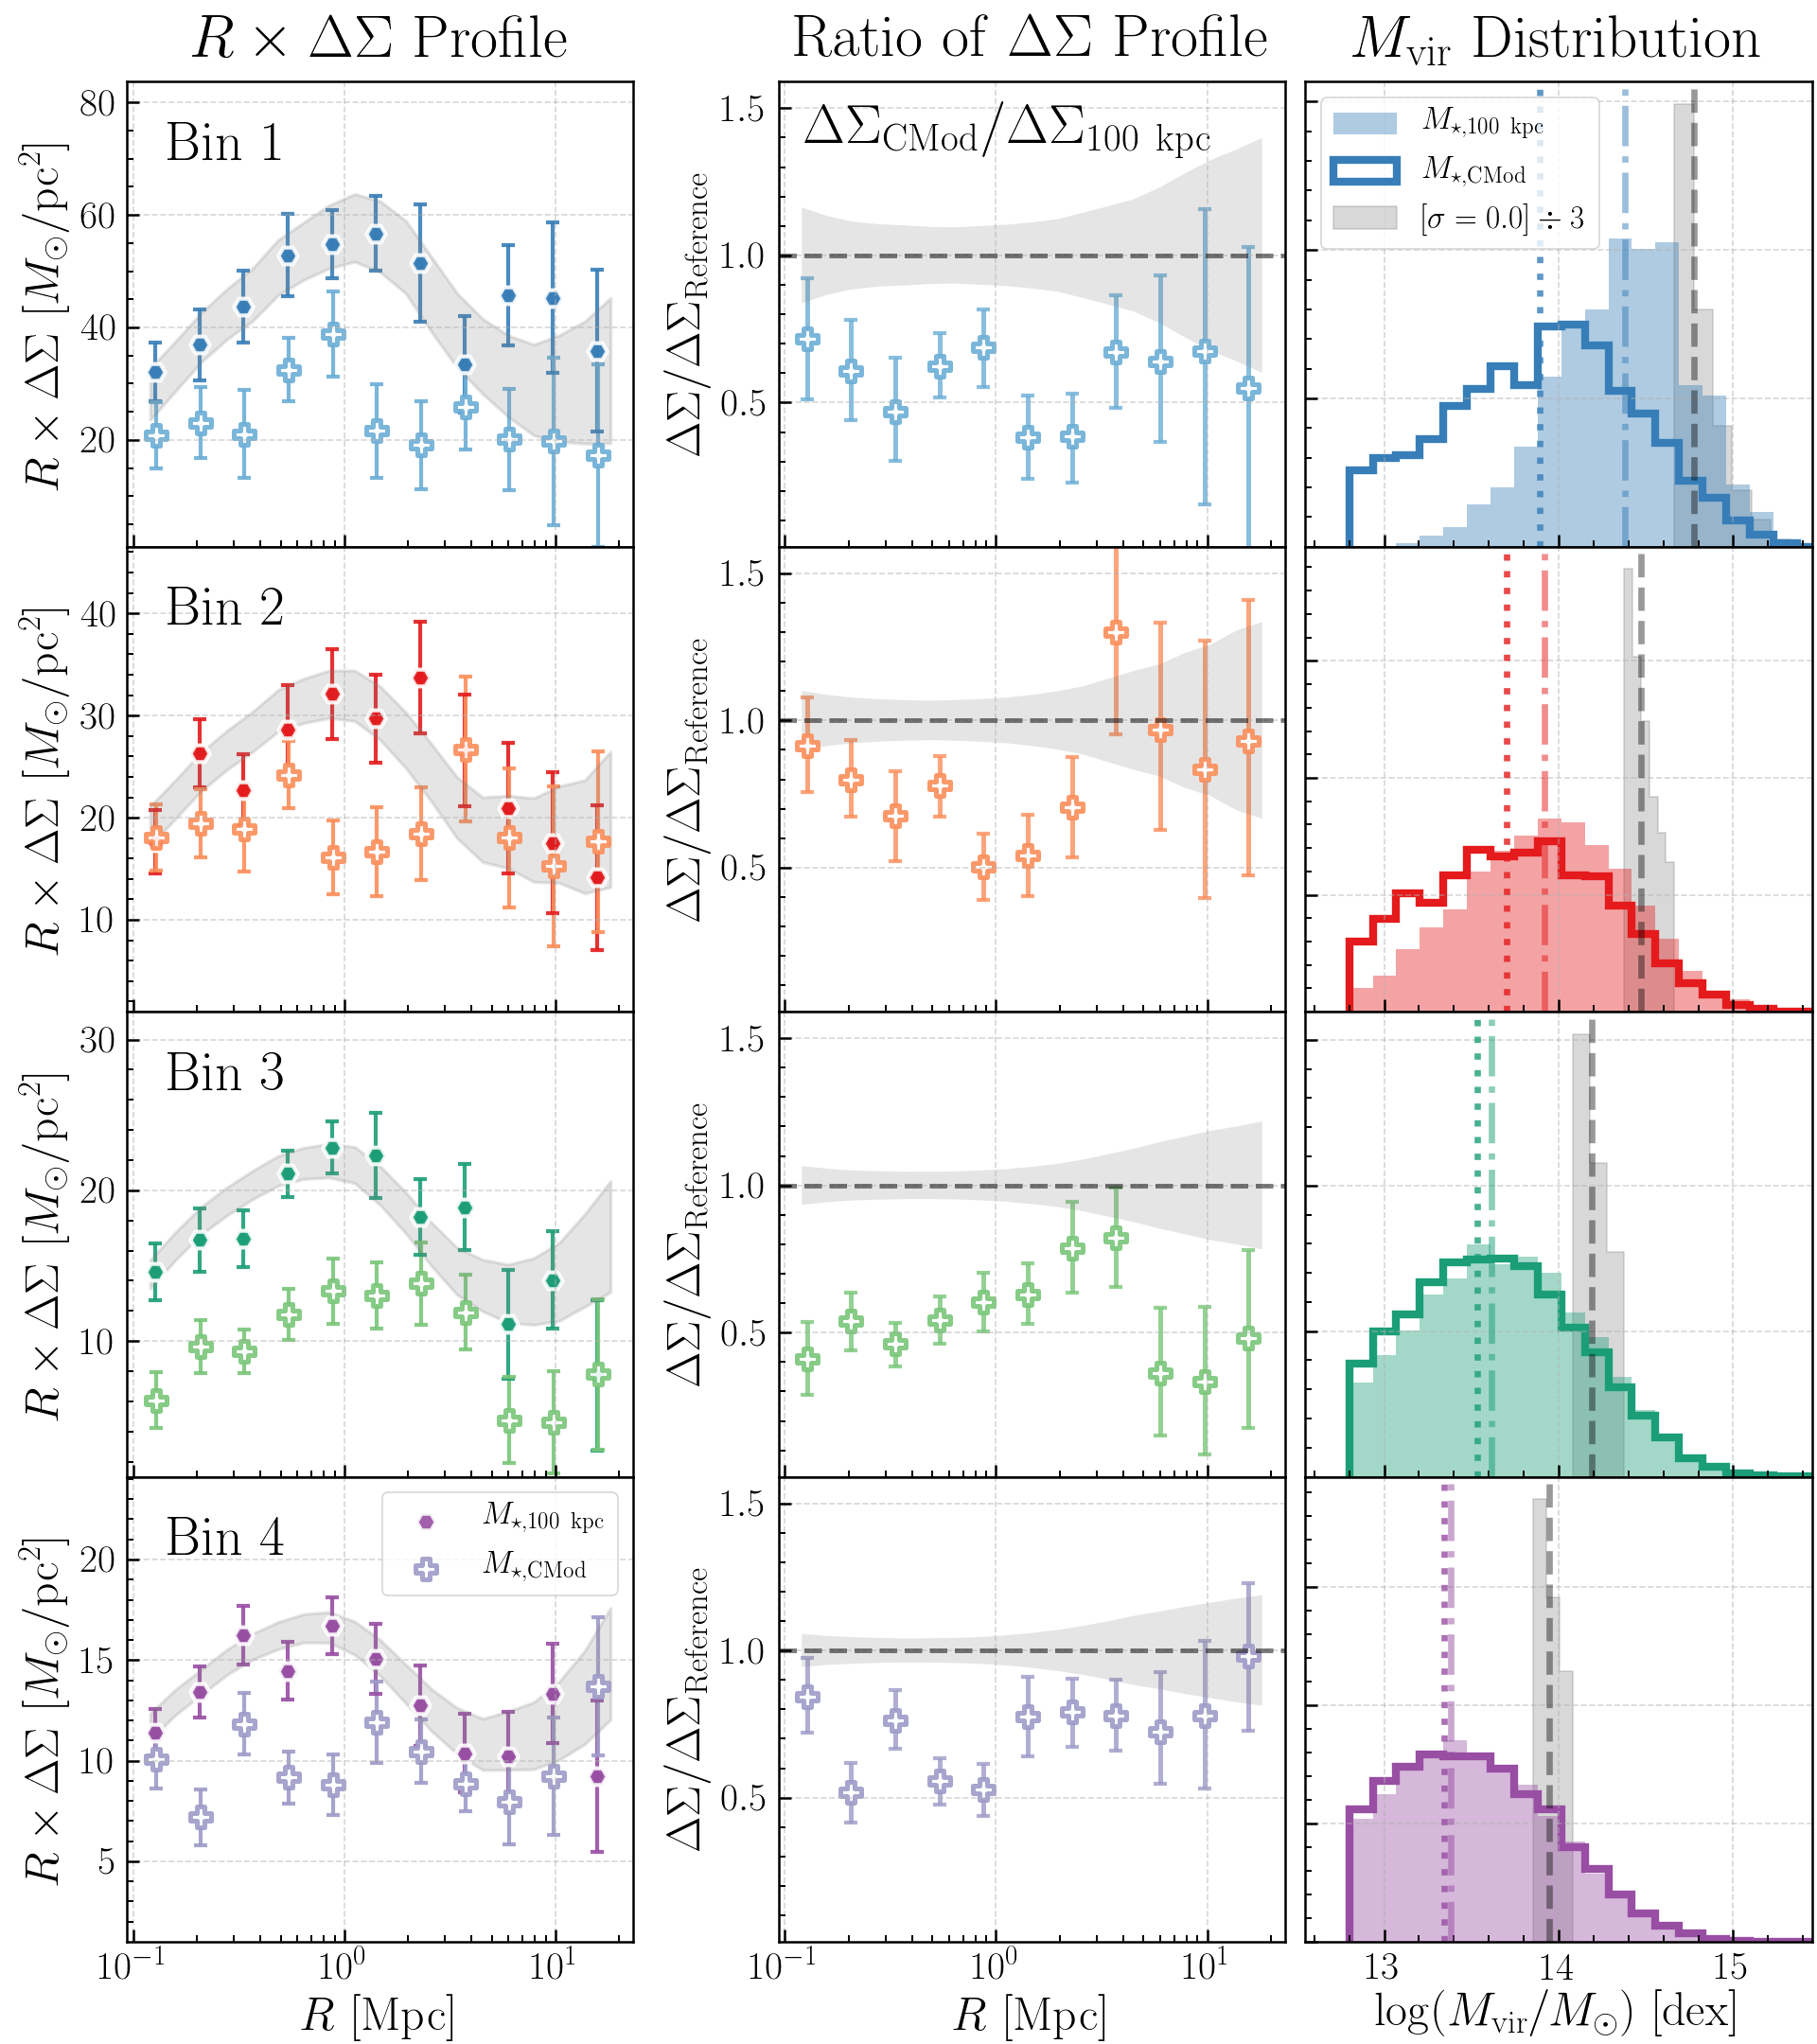
\includegraphics[width=\textwidth]{figure/topn_dsigma_m100_cmod_compare}
      \caption{
          \todo{Compare M100kpc and CModel mass}
          }
      \label{fig:m100_cmod}
  \end{figure*}
%% ---------------------------------------------------------------------------------------------- %%

%% ---------------------------------------------------------------------------------------------- %%
%% Poor performance of CModel stellar mass 
%% ---------------------------------------------------------------------------------------------- %%
\subsubsection{Performance of \mcmodel{}}
    \label{sec:cmodel}

    \todo{Fix the fitting results and the figure. In Bin 3 and 4, the \mvir{} distributions are 
        cut-off due to the \mdpl2{} limitation.}

    In the first section, we evaluate the performance of the \cmodel{} stellar mass as a 
    potential \mvir{} tracer.
    We compare the results for \mcmodel{} in the four number density bins with the ones for 
    the benchmark large aperture stellar mass \maper{100} in Figure \ref{fig:m100_cmod}.

    \plan{A detailed outline}

    \begin{itemize}
        
        \item In the left panels of Figure \ref{fig:m100_cmod}, we compare the \rdsigma{} profiles
            of the \mcmodel{}- and \maper{100}-selected samples. 
            Using the best-fit profiles as reference (gray shaded region), we can see that the 
            \dsigma{} profile of the \maper{100} samples are well-described by our simple model 
            within 1-$\sigma$ uncertainty. 
            The reduced \chisq{} values for the \maper{} samples are \todo{[XX, XX, XX, XX]}.
            This is an important point. It suggests that \emph{only} a Gaussian scatter around 
            the \mvir{}-observable relation can already explain the lensing signals at  
            the current \snratio{}.
            Such property makes it much easier to model and apply an observable as a \mvir{} proxy.
            In our tests, we see that most aperture-based \mstar{} fits this description. 
            In fact, \cmodel{}-selected galaxies also have \dsigma{} profiles well-fit by the model.
            Although it is hard to visualize in the figure, the reduced \chisq{} values for the 
            \mcmodel{} samples are \todo{[XX, XX, XX, XX]}.
        
        \item Meanwhile, in the same number density bin, the \mcmodel{}-based samples clearly have 
            much lower amplitudes in their \dsigma{} profiles compared to the \maper{100} ones.
            We highlight this using the middle panel of \ref{fig:m100_cmod}. 
            In all the four bins and at almost all radius, the \dsigma{} value of a \mcmodel{}-sample
            is $\sim$20-50\% lower than the \maper{100} one.
            Based on our model, this reflects the underlying difference of the \mvir{} distributions,
            where the \mcmodel{}-selected samples lower mean \mvir{} values and higher \sighalo{}
            than the \maper{100}-selected ones. 
            We visualize this in the right panels of \ref{fig:m100_cmod}.
        
        \item Limited by the sample size and the much lower \snratio{} of the \dsigma{} profiles 
            for the \mcmodel{} samples, we do not see any clear number density dependence or radial 
            trend of the difference.
            The \cmodel{} photometry based \mstar{} is a much worse \mvir{} tracer for nearby 
            massive galaxies in our test.
        
        \item The \sighalo{} values here apply only to the \cmodel{} photometry of HSC SSP 
            \texttt{S16A}. With a different imaging dataset, or a different treatment of background
            subtraction and deblending, we could get different \sighalo{} values in a similar test.
            Moreover, the credibility of \mcmodel{} as \mvir{} proxy should depend on the \mstar{}, 
            morphology, and redshift of the sample. For instance, it is potentially appropriate 
            to use \cmodel{} photometry for lower-\mstar{} or higher redshift samples.
            However, we do think the result here is consistent with the \emph{intrinsic} 
            limitation of \cmodel{} when fitting massive galaxies (e.g., \addref{}).
            It is well known that \cmodel{} photometry under-estimates the luminosity of a low-$z$
            massive galaxies (e.g., \addref{}).
            We hope to draw more attention to its impact in many aspects of galaxy-halo connection
            studies. We often see models calibrate their low-$z$ SHMR using \cmodel{} SMF of SDSS 
            galaxies, or a cluster-finder relies on \cmodel{} magnitude to assign central galaxy.
            These choices could have unintended consequence. 
             
    \end{itemize}

%% ---------------------------------------------------------------------------------------------- %%
%% Figure: Compare 50-100 kpc outer envelope mass and 100 kpc mass
%% ---------------------------------------------------------------------------------------------- %%
  \begin{figure*}
      \centering
      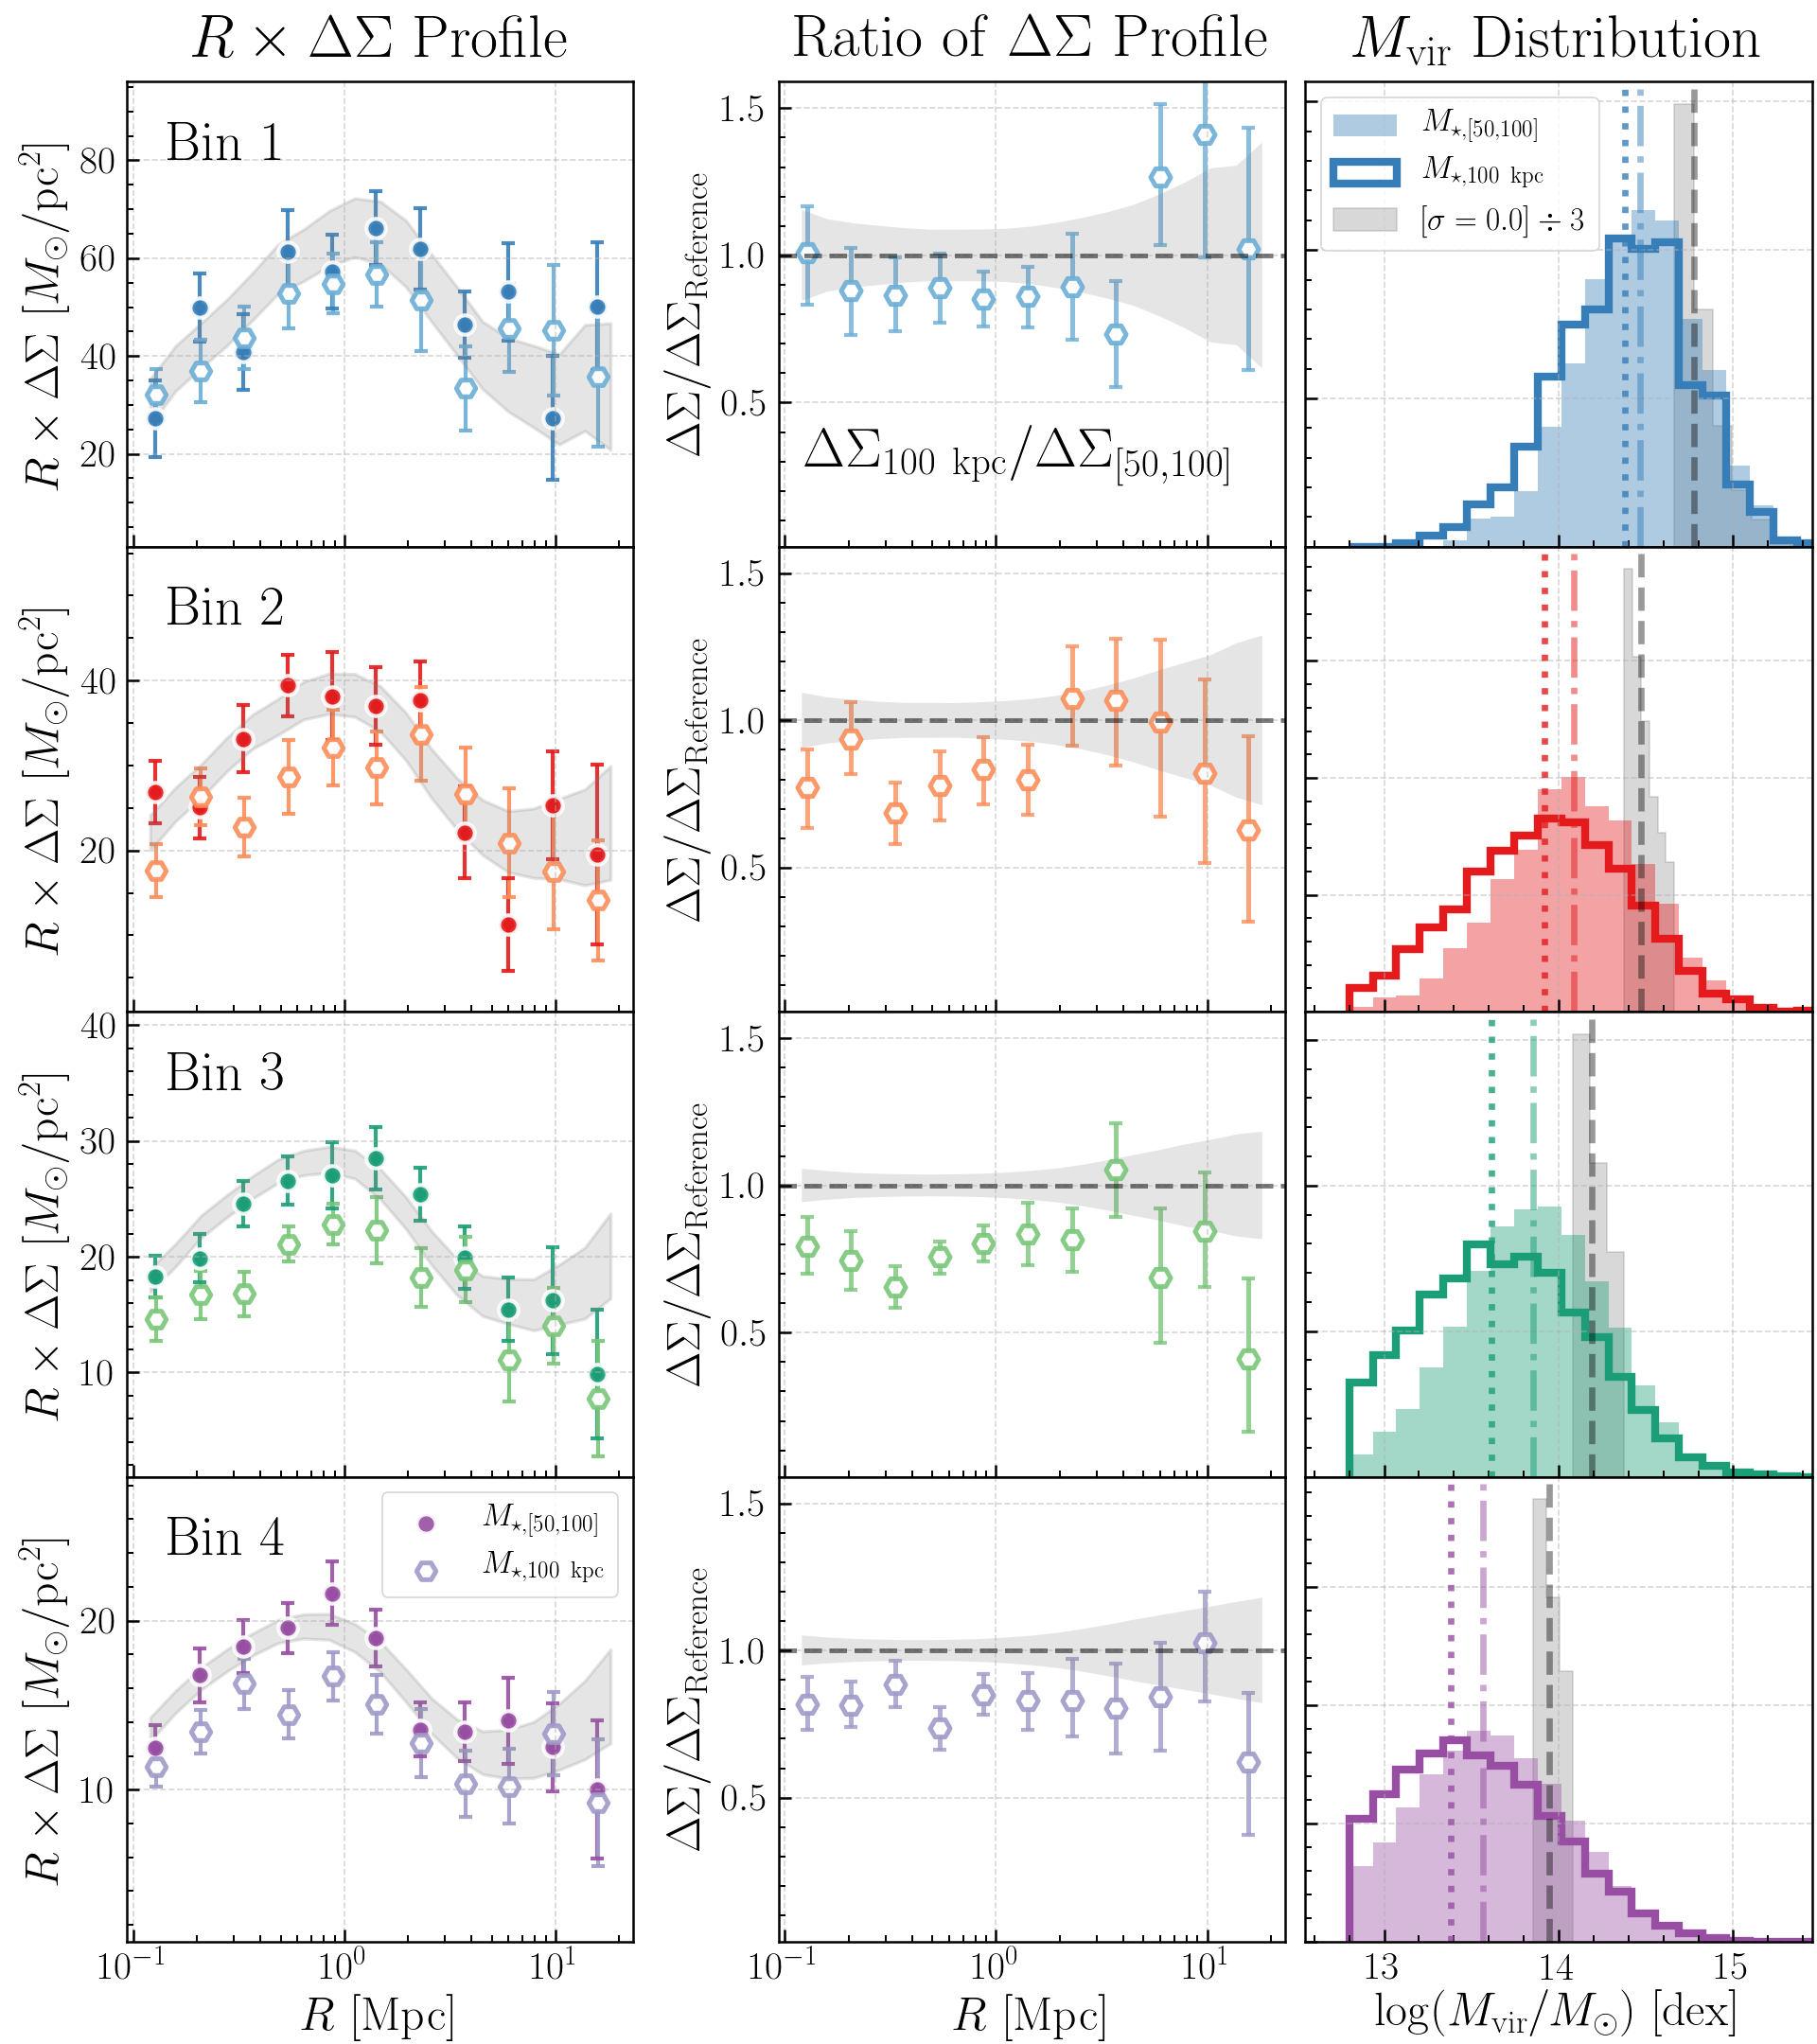
\includegraphics[width=\textwidth]{figure/topn_dsigma_m100_mout_compare}
      \caption{
          \todo{Compare 50-100 kpc outer envelope mass and 100 kpc mass}
          }
      \label{fig:m100_mout}
  \end{figure*}
%% ---------------------------------------------------------------------------------------------- %%

%% ---------------------------------------------------------------------------------------------- %%
%% Performance of outer envelope mass
%% ---------------------------------------------------------------------------------------------- %%
\subsubsection{Performance of the \mstar{} of outer envelope}
    \label{sec:moutskirt}

    \todo{Fix the fitting results and the figure. In Bin 3 and 4, the \mvir{} distributions are 
        cut-off due to the \mdpl2{} limitation.}
    
    \song{Should we try a similar one but based on Re, e.g. 2-4 Re instead of fixed aperture?
        or maybe R50 to R80?}

    In addition to the \mstar{} within large elliptical apertures, we also explore the possibility 
    of using \mstar{} within the \exsitu{}-star dominated outskirt as \mvir{} proxy.
    Here we use \menve{50}{100}, which is the \mstar{} between 50 and 100 kpc, as an example to 
    highlight the behaviour of outskirt \mstar{} (see Figure \ref{fig:m100_mout}).

    \plan{A detailed outline}

    \begin{itemize}

        \item Similar to \maper{100} and other aperture-based \mstar{}, \menve{50}{100} and other 
            outskirt \mstar{} can also select samples of massive galaxies whose \dsigma{} profiles
            are well-fit by our simple ``scatter-onky'' model (left panels of 
            Figure \ref{fig:m100_mout}).
        
        \item A little to our surprise, the overall amplitudes of the \dsigma{} profiles for the 
            \menve{50}{100} samples are consistently higher than the \maper{100} ones in all 
            bins. This conclusion does not change when we switch \maper{100} with \maper{150} or 
            \mmax{}. We highlight the ratios of the \dsigma{} profiles of these two samples in 
            the middle panels of Figure \ref{fig:m100_mout}. 
            There seems to be a slight radial dependence in the ratios (at least for the Bin
            1-3), where the difference is more significant in the inner 2-3 Mpc while the
            \dsigma{} profiles of the two samples roughly agree with each other at $R>5$ Mpc. 
            The difference in the inner region is also slightly stronger in Bin 2-4. 
            The average ratios \dsigma{}$_{100\ \rm kpc}/$\dsigma{}$_[50,100]$ for Bin [1, 2, 3, 4]
            are \todo{XX, XX, XX, XX}.
        
        \item Based on our model, this result suggests that, compared to \maper{100} and 
            aperture \mstar{} in general, outskirt \mstar{} like \menve{50}{100} can select 
            massive galaxies living in the halos with higher average \mvir{} and lower 
            \sighalo{} (as shown in the right panels of Figure \ref{fig:m100_mout}). 
        
        \item We rely on the low-\sb{} part of the surface brightness profile to estimate 
            the \mstar{} in the outskirt, which is more vulnerable to the relative large 
            statistical uncertainty in the photometry and systematic issues such as imperfect 
            background subtraction, contamination of nearby object, and the assumption of constant 
            \mlratio{}. It is reasonable to expect the \mvir{}-\menve{50}{100}
            relation is ``noisier'' than the one for aperture \mstar{}. 
            Therefore, the result highlighted in Fig \ref{fig:m100_mout} really demonstrate the 
            potential of using outskirt \mstar{} as a \mvir{} proxy.
            Given the likely case that the outskirts of massive galaxies are completely dominated 
            by \exsitu{} stars, this result could confirm that the \exsitu{} component can 
            predicts \mvir{} and trace the halo assembly better than the \insitu{} component. 
            Considering that \menve{50}{100} is included in \maper{100}, this may even suggest 
            that the \exsitu{} component or the outskirt \mstar{} are more useful than the 
            ``total'' \mstar{} when studying the galaxy-halo connection of massive galaxies.

        \item In this work, we only explore outskirt defined by two fixed physical radius.
            Such definition has the advantage of being unambiguous and straightforward. 
            Given unambiguous imaging data quality, it can be consistently apply to different 
            surveys too.
            The choices of these boundaries are subjective at best. 
            But we tested different definitions of outskirt \mstar{}, and the result is robust
            as long as the inner boundary is larger than 50 kpc.
        
        \item Meanwhile, ``outskirt'' definition with an inner boundary of 50 kpc makes it 
            difficult to extend this proxy to lower-\mstar{} or higher-redshift galaxies.
            And the \exsitu{} fraction within \menve{50}{100} at different \mstar{} is still 
            unknown. It is worth exploring alternative definitions of outskirt (e.g., relative
            to $R_{\rm e}$ or $R_{80}$) or ``calibrating'' the definition using the
            state-of-the-art hydro-simulation to reflect the underlying \exsitu{} \mstar{} better.

    \end{itemize}

%% ---------------------------------------------------------------------------------------------- %%
%% Figure: Comparisons of scatters: different tracers and aperture masses
%% ---------------------------------------------------------------------------------------------- %%
  \begin{figure*}
      \centering 
      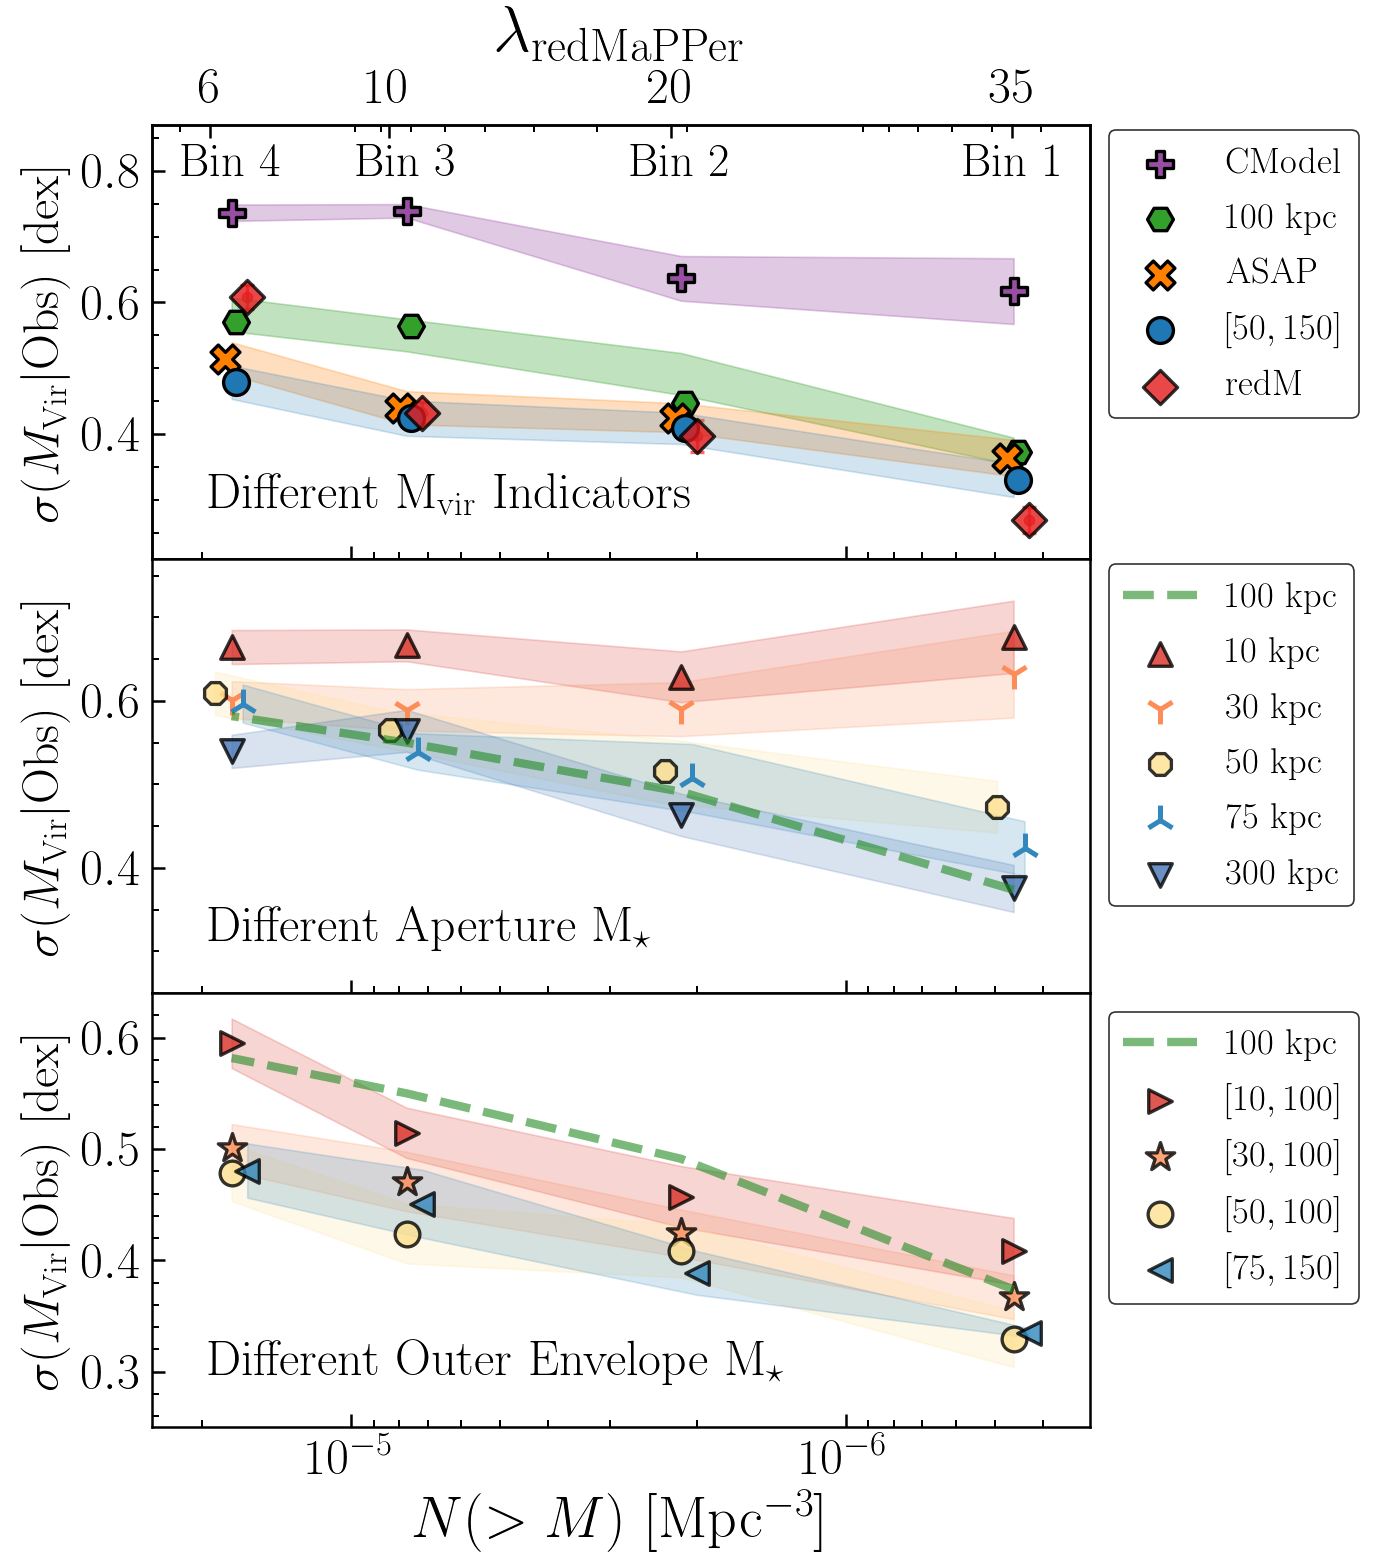
\includegraphics[width=0.85\textwidth]{figure/topn_sigma_trend_sum}
      \caption{
          \todo{Comparisons of scatters: different tracers and aperture masses.}
          }
      \label{fig:scatter_trend}
  \end{figure*}
%% ---------------------------------------------------------------------------------------------- %%


%% ---------------------------------------------------------------------------------------------- %%
%% General trends of scatters
%% ---------------------------------------------------------------------------------------------- %%
\subsubsection{Scatter of \mvir{} at Fixed Observables}
    \label{sec:trend}

    As a summary of the ``Top N'' test results, we highlight the relationships between 
    \sighalo{} and the number density for three groups of different \mvir{} proxies explored in 
    this work in Figure \ref{fig:scatter_trend}.
    We also record the ranges of observables in each bin and their \sighalo{} values in 
    Table \ref{tab:summary}.
    
    \todo{Figure needs to be updated with the new models}

    We want to emphasis again that, for all the \mstar{}-based observables, we \emph{do not
    exclude} massive satellite galaxies in both the observations and the simulations. 
    We show in \S \ref{sec:satellite} that, due to the low satellite fraction at high-\mstar{}
    end, we see no impact on the \dsigma{} profiles for Bin 1 \& 2 and visible but small ($<20$\%)
    effect at $R>2$-3 Mpc in Bin 3 \& 4.
    
    \plan{A detailed outline}

    \begin{itemize}

        \item In the upper panel, we compare the representative \mvir{} proxies from several different 
            disciplines including the \mstar{} based on default survey photometry (\mcmodel{}), 
            the \mstar{} within large elliptical aperture (\maper{100}), the \mstar{} in the outskirt of 
            massive galaxies (\menve{50}{100}), the \mvir{} predicted by simple empirical 
            model (\masap{}), and the richness of red-sequence galaxies 
            ($\lambda_{\rm redM,\ HSC}$).
            Ignoring the subtle differences in the \dsigma{} profiles for now, we consider 
            the observable with lower \sighalo{} value in the same density bin a better massive halo 
            tracer (or ``cluster finder'').
        
        \item Using the ``Top N'' tests, we confirm that the richness of red-sequence galaxies is indeed 
            an excellent \mvir{} proxy in the \mvir{} regime for galaxy clusters ($>10^{14} M_{\odot}$).
            All the three red-sequence cluster finders show lower \sigmh{} values in Bin 1 \& 2 
            than the \mstar{}-based \mvir{} proxies.
            In Figure \ref{fig:scatter_trend}, we only show the results for the HSC \texttt{S16A}
            \redm{} clusters, which have \sigmh{}$=$[\todo{XX, XX}] for Bin [1, 2]. 
            For the HSC \camira{} clusters (SDSS \redm{} \texttt{v6.3} clusters), the \sigmh{} values are 
            [\todo{XX, XX}] (\todo{XX, XX}) for Bin [1, 2].
            In the lower \mvir{} end, we find evidence that the performance of richness as massive halo 
            finder becomes similar or even slightly worse than certain \mstar{}-based \mvir{} proxy that 
            will be discussed later.
            The HSC \redm{} clusters have \sigmh{}$=$[\todo{XX, XX}] in Bin [3, 4], while the \camira{}
            clusters have \sigmh{}$=$\todo{XX} in Bin 3.
            We should note that the HSC \redm{} catalog attempts to reach down to extremely low richness 
            that is challenging for any ``cluster'' finder and it has not been thoroughly vetted.
            But the increasing trend of \sigmh{} with decreasing richness is qualitatively consistent 
            with recent calibrations of \mvir{}-richness relations for both \redm{} 
            (e.g., \citealt{Murata2018}; Figure 11) and \camira{} (e.g., \citealt{Murata2019}; Figure 12)
            catalogs using a more sophisticated forward-modeling scheme.
            \song{We could compare the scatter values too. Our scatter values in the Bin 1 \& 2
            are consistent with Murata et al. 2018 for \redm{} but are slightly higher than 
            Murata et al. 2020 for \camira{}. We just need to convert the $\sigma_{\ln M_{\rm vir}}$ into
            our $\log$ one, and also try to account for the binning effect (or just use the mean richness
            value)}.
            Notwithstanding such low \sigmh{} values in the galaxy cluster regime, we also notice interesting
            and systematic differences in the \dsigma{} profiles between \mstar{}- and richness-selected 
            halos. We will discuss this later in \S \ref{sec:mstar_vs_richness}.

        \item As already highlighted in \S \ref{sec:cmodel}, \maper{100} is clearly a much better 
            \mvir{} proxy in all four bins. Meanwhile, the outskirt stellar mass \menve{50}{100}
            out-performs \maper{100} especially in Bin 2, 3, \& 4, which is also consistent with the 
            qualitative conclusion from comparing their \dsigma{} profiles in \S \ref{sec:moutskirt}.
            In addition, for all the \mstar{}-based \mvir{} proxies shown in this panel, their \sighalo{}
            values become lower with decreasing number density thresholds (or from Bin 4 to 1).
            This suggests that the (intrinsic) scatter of SHMR decrease with \mvir{} at the high-mass end,
            which is consistent with the \todo{...comparison with a few recent works, both observations 
            and simulation. Also, technically, we do not know whether the slope of the SHMR varies too.}
        
        \item From these comparisons, we reinforce two important conclusions.
            Firstly, when the imaging quality allows, \mstar{} out to large physical aperture or
            just in the very outskirt of massive galaxies can serve as a better \mvir{} proxy to
            study galaxy-halo connection than \mstar{} based on default photometry.
            This finding has implications in many on-going and future imaging surveys and can apply 
            to photometric methods other than \cmodel{}. 
            Small matched aperture photometry, default photometry from \texttt{SExtractor}, or even 
            single-\ser{} model can still have systematic issues at different levels for massive
            galaxies. We will investigate into these issues in future works.
            Secondly, the ``Top N'' tests consistently show that the \mstar{} in different parts of 
            low-$z$ massive galaxies follow different SHMR. 
            The \exsitu{} star dominated outskirt shows a closer relation to its dark matter halo.
        
        \item To further demonstrate the second point, we compare the results for different
            aperture \mstar{} and different outskirt \mstar{} in the middle and bottom panels of
            Figure \ref{fig:scatter_trend}. For aperture \mstar{}, the \sighalo{} at fixed number
            density significantly decreases with increasingly large aperture value, especially in Bin
            1 \& 2. For Bin 1, \sighalo{} decreases from \todo{XX} for \maper{10 kpc}, and \todo{XX}
            for \maper{30}, to \todo{XX} for \maper{100} (green dashed line as reference). The
            \sighalo{} values for \maper{10} and \maper{30} do not decrease with volume number
            density as well.
            In the current data, aperture \mstar{} defined by $R>100$ kpc, including the one based on 
            extrapolation to 300 kpc with a single-\ser{} model fit to the outskirt (\maper{300}), 
            does not lead to unambiguous improvement of \sighalo{} value.
            It is unclear whether this reflects the intrinsic properties of stellar halo in massive 
            galaxies or it is simply due to systematic limitation related to imaging quality or 
            data reduction \song{Using the \mstar{} between 100 and 150, or 300 kpc can test this}. 
            Meanwhile, the bottom panel shows that stellar outskirt \mstar{} outperforms 
            \maper{100} as long as the inner boundary is larger than $\sim 30$-50 kpc. 
            All together, these comparisons show that the outer stellar halos of nearby massive 
            halos ``care'' about their dark matter halos much more than their central region. 
        
        \item In the top panel of Figure \ref{fig:scatter_trend}, we show that the \asap{} model 
            also provides a reasonably good \mvir{} proxy whose \sighalo{} values
            are better than \maper{100} and on a par with the \menve{50}{100}. 
            Though not displayed here, our ``scatter-only'' \mvir{}-observable model can fit 
            the \dsigma{} profiles of \masap{}-selected samples very well \todo{Put relevant figures 
            in Github and provide a link}.
            This is not a surprise given the 2-D scaling relation derived from the \asap{} model is 
            also based on two aperture \mstar{}.
            The improvement compared to single aperture \mstar{} confirms the result of 
            \citet{Huang2020}.
            In \citet{Huang2020}, we essentially utilize the outskirt \mstar{} with a 10 kpc inner 
            boundary. 
            Given the results of this work, there should be rooms to further improve
            phenomenological model like \asap{} by focusing on outer stellar halo such as between
            50 to 100 kpc.
            Meanwhile, several systematic issues in the \um{} model adopted by \citet{Huang2020},
            and the current sample size at the highest-\mstar{} end could also be the limiting 
            factors for using \asap{} model as a ``cluster finder''.
        
    \end{itemize}


%% ---------------------------------------------------------------------------------------------- %%
%% Figure: Compare 50-100 kpc outer envelope mass and richness selected clusters
%% ---------------------------------------------------------------------------------------------- %%
  \begin{figure*}
      \centering
      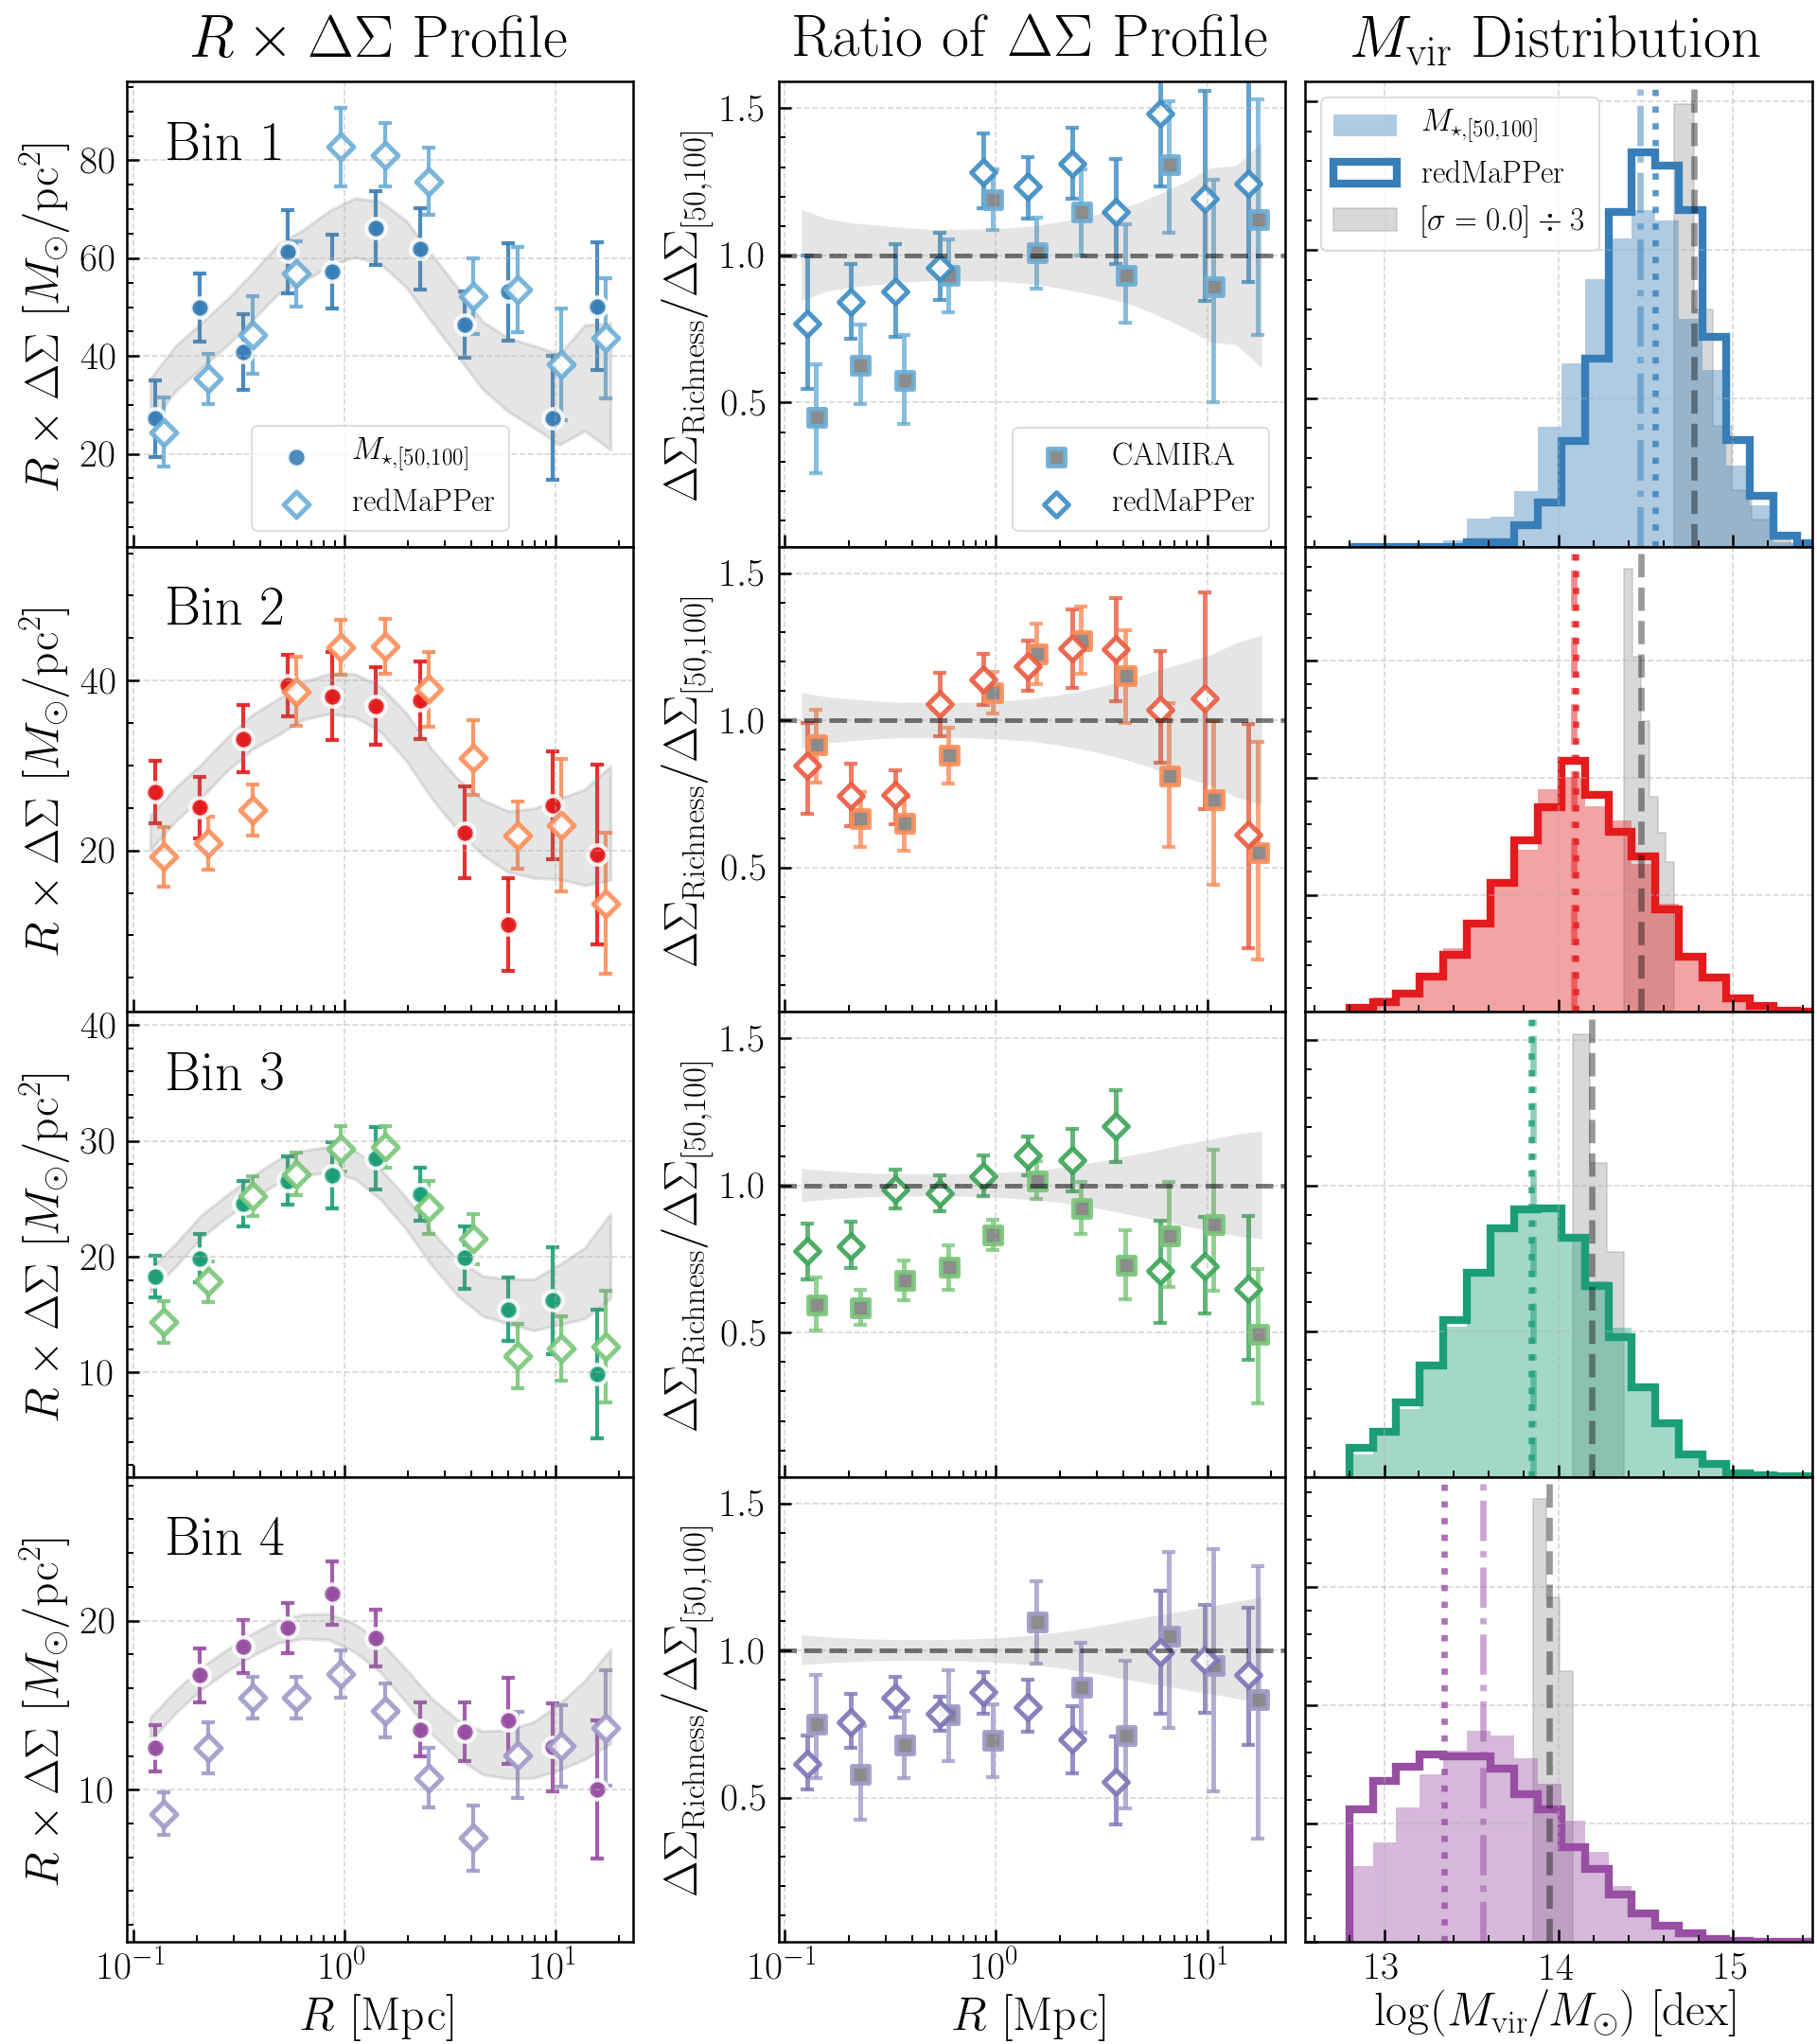
\includegraphics[width=\textwidth]{figure/topn_dsigma_mout6_redm_compare}
      \caption{
          \todo{Compare 50-100 kpc outer envelope mass and richness selected clusters}
          }
      \label{fig:mout_richness}
  \end{figure*}
%% ---------------------------------------------------------------------------------------------- %%

%% ---------------------------------------------------------------------------------------------- %%
%% Figure: Compare the DSigma profiles of richness selection clusters with their 
%%		   best-fit model.
%% ---------------------------------------------------------------------------------------------- %%
  \begin{figure*}
      \centering
      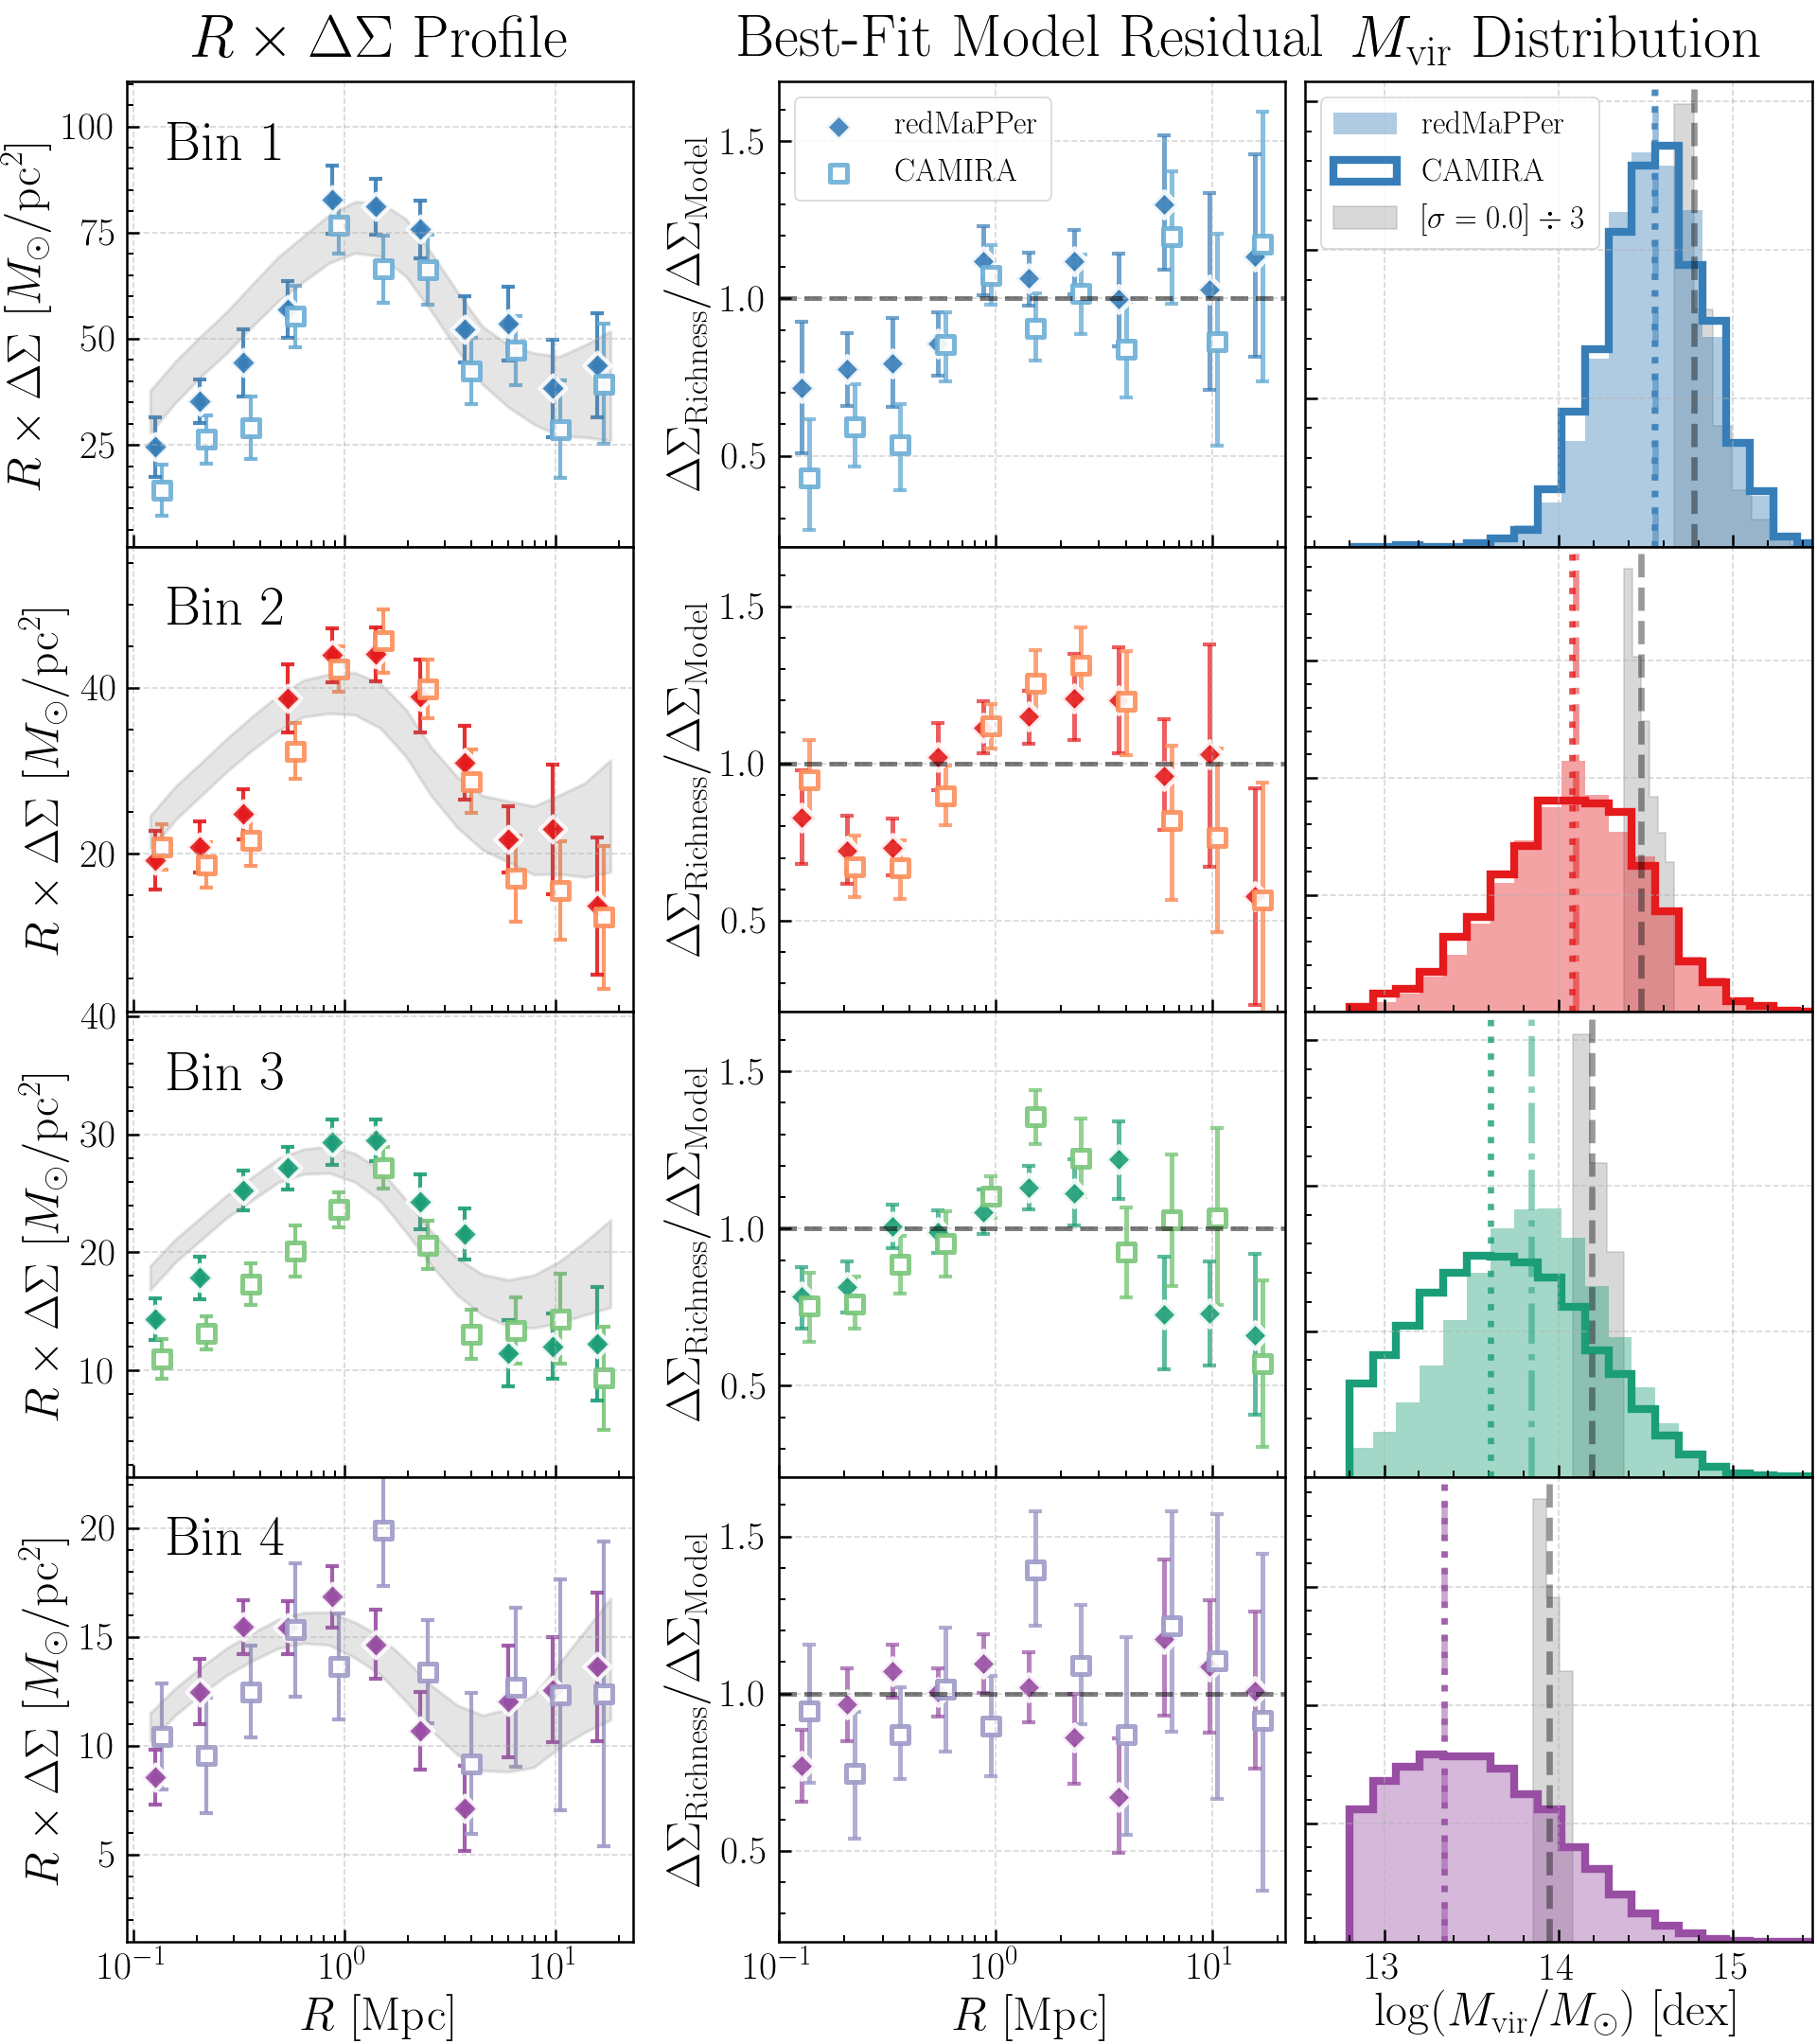
\includegraphics[width=\textwidth]{figure/topn_dsigma_redm_cam_residual}
      \caption{
          \todo{Compare the DSigma profiles of richness selection clusters with their 		   
          		best-fit model.}
          }
      \label{fig:richness_residual}
  \end{figure*}
%% ---------------------------------------------------------------------------------------------- %%
    
%% ---------------------------------------------------------------------------------------------- %%
%% Comparison with richness selected galaxies
%% ---------------------------------------------------------------------------------------------- %%
\subsection{The $\Delta\Sigma$ Profiles of \mstar{} and Richness Selected Samples}
    \label{sec:mstar_vs_richness}

    \todo{Update Figure \ref{fig:richness_residual} and Figure \ref{fig:mout_richness}:
        remove the \camira{} points in Bin 4.}

    In this section, we will take a closer look at the \dsigma{} profiles of the
    richness-selected massive halos with two key questions in mind:

    \begin{enumerate}

        \item What is the difference between the \dsigma{} profiles of massive halos selected 
            by richness and \mstar{} in the same number density bins?

        \item Can we use a simple $\log$-linear \mvir{}-richness relation with Gaussian 
            scatter to explain the \dsigma{} profiles of richness-selected clusters?

    \end{enumerate}

    \plan{Rough outline}

    \begin{itemize}

        \item In \S \ref{sec:trend} and Figure \ref{fig:scatter_trend}, we show that
            \redm{} (both the HSC and SDSS one) and \camira{} red-sequence cluster finders 
            have better performance at the very high-\mvir{} end of HMF than any \mstar{}-based
            massive halo tracer.
            In this case, we expect the \dsigma{} profiles of richness-selected clusters to 
            have higher overall amplitudes than the \mstar{} selected ones in the same bin 
            due to the higher average \mvir{}.
            At lower-\mvir{} regime, the \mstar{}-based \mvir{} proxies, especially the outskirt
            \mstar{} such as \menve{50}{100}, start to demonstrate comparable (Bin 2 \& 3) 
            \sigmh{} performance to the richness-based ones. 
            Therefore, we expect to see similar \dsigma{} profiles.
        
        \item In the left panels of Figure \ref{fig:mout_richness}, we compare the \dsigma{}
            profiles of HSC \redm{} clusters and \menve{50}{100}-selected massive halos in the four
            density bins.
            To highlight the differences better, we show the ratios between the \dsigma{} profiles 
            of the richness-selected samples and the \menve{50}{100} ones using both 
            HSC \redm{} and \camira{} (only for Bin 1--3) clusters.
            SDSS \redm{} clusters are also consistent with these results in the first two bins.
            \todo{Make figures available in Github and provide the links}.
            Interestingly, we see similar and systematic differences in their \dsigma{} 
            profiles in Bin 1-3: although the average amplitudes are similar within 
            $R < 5$ Mpc, the richness-selected clusters have $\sim 20$-40\% lower \dsigma{} amplitudes than 
            the \menve{50}{100}-selected galaxies in the $R < 1$ Mpc inner region.
            The \camira{} \dsigma{} profiles show slightly stronger ``dipping'' in this region 
            than the \redm{} ones (especially in Bin 1 \& 3).
            Meanwhile, both \redm{} and \camira{} profiles show enhanced \dsigma{} profiles in the 
            $1 < R < 3$ Mpc regime in Bin 1 \& 2 at about 20-30\% level.
            The sample sizes are still quite limited for both Bin 1 \& 2, but the consistent features 
            found in different red-sequence finders suggest that this is a robust result.
            The similarity between the \redm{} and \camira{} profiles in Bin 2 is remarkable.
            For Bin 3, the \redm{} and \camira{} \dsigma{} profiles have amplitudes similar 
            to the \menve{} one at $1 < R < 3$ Mpc.
        
        \item At $R > 5$ Mpc, we are still limited by the \snratio{} of the \dsigma{} profiles 
            from both observations and simulations, so the result is still a little uncertain.
            In Bin 1 with only 49 systems, the outer \dsigma{} profiles of richness- and 
            \menve{50}{100}-selected samples are statistically consistent with each other.
            Meanwhile, we find marginal evidence that the \dsigma{} profiles of the \redm{} and 
            \camira{} clusters become lower than the \menve{50}{100} galaxies at $R > 5$ Mpc 
            in Bin 2 \& 3. 
            The fact that we see this similar, albeit noisy, trend using different cluster finders
            makes it worth investigating further.

        \item The \dsigma{} profile of \redm{} samples in Bin 4 starts to globally fall below the 
            \menve{50}{100}-selected halos as indicated by the \sigmh{} measurements shown in 
            Figure \ref{fig:scatter_trend}.
            Halos in Bin 4 have average \logmh{}$<13.8$ for all our \mvir{} proxies. 
            In this ``massive group'' regime, it is not surprising to see richness-based cluster
            finder start to face intrinsic limitation caused by low and noisy richness level 
            and become more vulnerable to systematic issues (e.g. photo-$z$ uncertainty, 
            projection effect).
        
        \item We should note that the seemingly diffrent behavior between Bin 2 and 3 is partly
            due to the usage of \menve{50}{100} for comparison in stead of large aperture \mstar{}.
            We already demonstrated that \menve{50}{100} is a better \mvir{} tracer than \maper{100},
            \maper{150}, or \mmax{} in \S \ref{sec:moutskirt} and \S \ref{sec:trend}.
            In Figure \ref{fig:m100_mout}, the \dsigma{} profiles of \menve{50}{100} samples are 
            consistently $\sim 10$--30\% higher than the \maper{100} ones.
            When replacing \menve{50}{100} with \maper{100} in Figure \ref{fig:mout_richness}, 
            we can see that, compared to the \dsigma{} profiles of \mstar{}-selected samples, 
            the ones for richness-selected clusters always show ``suppressed'' signal at 
            $R < 1$ Mpc and ``enhanced'' \dsigma{} at $1 < R < 3$ Mpc.
            \todo{Provide the link to this figure}
            For Bin 2 \& 3, we can see a ``bump''-like feature right outside 1 Mpc, which happens
            to correspond to the rough boundary between the 1-halo and 2-halo term for cluster-mass
            halos. 
            Regardless the cause of this trend (see discussion in \S 
            \ref{sec:cause_of_difference}), this result reveals potentially important difference 
            between the halos identified by the \mstar{} of their central galaxy and the ones 
            by the richness of galaxies in them \emph{at similr average \mvir{}}.

        \item To address question two, we compare the \dsigma{} profiles of richness-selected clusters
            with their best-fit profiles from our model.
            The left panels of Figure \ref{fig:richness_residual} compares the \dsigma{}
            profiles of HSC \redm{} and \camira{} clusters in each bin.
            It is clear that the simple ``$\log$-linear \mvir{}-observable with Gaussian scatter''
            model can not fit the observed \dsigma{} profiles well.
            The reduced \chisq{} values for the \redm{} (\camira{}) clusters in the four bins are 
            \todo{[XX, XX, XX, XX]} (\todo{[XX, XX, XX, XX]}).
            The deviations from the ``best-fit'' profiles are not only very significant, but also
            clearly resemble the differences with \mstar{}-based samples described above.
            And as the model profile is much less noisier, we can see the systematic trends in
            these deviations clearly using the relative ``residual'' profiles in the middle panels 
            of Figure \ref{fig:richness_residual}:
            1) In the highest-\mvir{} Bin 1, we see the \dsigma{} profiles are supressed inside 
            1 Mpc by up to $\sim 50$\% compared to the ``scatter''--only model profile. The $R > 1$
            Mpc parts, on the other hand, are well-fit by the model.
            2) In Bin 2 \& 3, the most prominent feature is the ``bump'' around 1-2 Mpc.
            The richness-selected clusters here show suppressed \dsigma{} profiles at both inner and 
            outer regions.
            3) In Bin 4, the \redm{} clusters show statistically consistent \dsigma{} profile with 
            the model. Although there could be weak evidence of supressed \dsigma{} signals at 
            $R < 200$ kpc and $2 < R < 4$ Mpc.

        \item The \redm{} and \camira{} \dsigma{} profiles are consistent within 1-$\sigma$ 
            uncertainties in Bin 1 \& 2 (\camira{} tends to show slightly lower amplitudes).
            In Bin 3, the \camira{} profile is significantly lower than the \redm{} one by
            $\sim 20-30$\% at $R < 1$ Mpc. 
            However, regardless of these differences, their ``residuals'' compared to our 
            ``scatter''--only model are remarkably similar. 
            This reinforce our conclusion: compared to the \mstar{}-based \mvir{} proxies whose 
            \dsigma{} profiles are adequately depicted by our simple model, the richness-based 
            cluster finders show systematic difference in their \dsigma{} profiles, suggesting 
            a $\log$--normal \mvir{}-richness relation with Gaussian scatter does not fully capture 
            the \mvir{} distribution.
            This result is in line with previous models for cluster lensing signals 
            (e.g., \citealt{Murata2019}, \addref{}), but to our best knowledge, this is the first 
            time it has been illustrated without assuming the contributions from different 
            ``components'' in the \dsigma{} profile.

    \end{itemize}
   
    We should mention that the statistical uncertainties of the model \dsigma{} profile 
    using \mdpl2{} and \smdpl{} simulations have been increased to match the volume of 
    HSC \texttt{S16A} sample.
    With increasingly larger sky coverage of HSC survey (e.g. $>600$ deg$^2$ of FDFC region 
    in \texttt{S19A} compared to $\sim 137$ deg$^2$ in \texttt{S16A}), future sample can 
    exame these systematic differences more precisely. 
    We will briefly discuss the potential causes of such differences and their implications
    in \S \ref{sec:cause_of_difference} and \S \ref{sec:perfect_finder}.

%% ---------------------------------------------------------------------------------------------- %%
%% Discussion 
%% ---------------------------------------------------------------------------------------------- %%
\section{Discussion}
    \label{sec:discussion}


%% ---------------------------------------------------------------------------------------------- %%
%% Discussion about the outer envelope mass
%% ---------------------------------------------------------------------------------------------- %%
\subsection{Outer Galaxy Mass}
    \label{sec:outer_mstar}

    Discuss here why we think the outer mass may work the best. Is this because of the
    \textbf{slope} of the $Mexsitu$ verus Mhalo plane being steeper than for insitu mass (see
    plot in Chris paper). Can discuss how UM and TNG predictions are different in this regard.

    \todo{Figure: show a figure of the ASAP model but using the outer mass. Is the boundary more 
        clear? Is this what ASAP was telling us all along?}

    \plan{Rough outline}

    \begin{itemize}

        \item Relation with \exsitu{} stellar mass and the problem. 

        \item Relation with ``ICL'' \mstar{}.

    \end{itemize}

%% ---------------------------------------------------------------------------------------------- %%
%% Discuss the difference between richness and stellar mass selections 
%% ---------------------------------------------------------------------------------------------- %%
\subsection{Outer Galaxy Mass}
    \label{sec:cause_of_difference}



%% ---------------------------------------------------------------------------------------------- %%
%% A ``perfect'' cluster finder?
%% ---------------------------------------------------------------------------------------------- %%
\subsection{What is an ``Ideal'' Cluster Finder?}
    \label{sec:perfect_finder}

    \plan{Rough outline}

    \begin{itemize}

        \item \plan{
            \citet{Rykoff2014} outlined a few requirements for an ideal richness cluster 
            finder. We will review it again with the results of this work in mind.
        }

        \item How does this change how we think about optical cluster finding?

        \item Importance of measuring total luminosity. Crappiness of Cmodel. 
        
        \item What are the current limitations: Ability to deal with galaxy with complex 
            morphology, in mergers, double core, or simply has too much contamination.


        \item Chris paper: but selection by $M*$ could be more subject to assembly bias

        \item Baryonic effects can be discussed here
    
        \item Cen$+N$? Magnitude gap? ``Total'' \mstar{} (there is a recent paper on this)?
            Size (We know it is not that good)? Or stellar velocity dispersion (also not very good)?

        \item Could take a look of the common and different ones in each bin. Using their 
            lensing signal as guidance: in \redm{}; not in \mstar{} v.s. in \mstar{}; not in \redm{}

    \end{itemize}

%% ---------------------------------------------------------------------------------------------- %%
%% ---------------------------------------------------------------------------------------------- %%
\subsection{Comparison with X--ray observation}
    \label{sec:xray}

    \alexie{We are going to think about whether to add this here or not. Deceide later.}
    \song{I think we should save this for later, maybe mentioning it as ``future work''}


%% ---------------------------------------------------------------------------------------------- %%
%% Summary 
%% ---------------------------------------------------------------------------------------------- %%
\section{Summary and Conclusions}
    \label{sec:summary}
    
    % Main conclusion    
    \plan{A detailed outline}    

    In this work, 

    In these tests, we directly compare he \dsigma{} profiles of massive halos identified 
    by different \mvir{} proxies in the same number density bins. 
    The overall amplitudes of the \dsigma{} profiles reflect both the average \mvir{} and the 
    \sighalo{} of the underlying samples, therefore can help us exam the capabilities of 
    different observables as \mvir{} proxies.
    We also develop a simple toy-model based on dark matter N-body simulations to predict 
    \dsigma{} profile\todo{...|}

    % Future direction   
    \todo{Briefly mention a few future directions. Also name as many as I can think of, 
          need to pick a few.}

%% ---------------------------------------------------------------------------------------------- %%
%% Acknowledgements 
%% ---------------------------------------------------------------------------------------------- %%
\section*{Acknowledgements}

  % Personal 
  \todo{The authors would like to thank XXX for useful discussions and suggestions.}

  % NSF funding
  This material is based upon work supported by the National Science Foundation under 
  Grant No. 1714610. 
  
  % KITP
  The authors acknowledge support from the Kavli Institute for Theoretical Physics.
  This research was also supported in part by National Science Foundation under Grant 
  No. NSF PHY11-25915 and Grant No. NSF PHY17-48958
  
  % AL's funding 
  We acknowledge use of the lux supercomputer at UC Santa Cruz, funded by NSF MRI grant AST
  1828315. AL is supported by the U.D Department of Energy, Office of Science, Office of High
  Energy Physics under Award Number DE-SC0019301. AL acknowledges support from the David and
  Lucille Packard foundation, and from the Alfred .P Sloan foundation.

  % HSC part
  The Hyper Suprime-Cam (HSC) collaboration includes the astronomical communities of 
  Japan and Taiwan, and Princeton University.  The HSC instrumentation and software were
  developed by National Astronomical Observatory of Japan (NAOJ), Kavli Institute
  for the Physics and Mathematics of the Universe (Kavli IPMU), University of Tokyo,
  High Energy Accelerator Research Organization (KEK), Academia Sinica Institute
  for Astronomy and Astrophysics in Taiwan (ASIAA), and Princeton University.  
  Funding was contributed by the FIRST program from Japanese Cabinet Office,  Ministry 
  of Education, Culture, Sports, Science and Technology (MEXT), Japan Society for 
  the Promotion of Science (JSPS), Japan Science and Technology Agency (JST), Toray 
  Science Foundation, NAOJ, Kavli IPMU, KEK, ASIAA, and Princeton University.
   
  % SDSS part
  Funding for SDSS-III has been provided by Alfred P. Sloan Foundation, the 
  Participating Institutions, National Science Foundation, and U.S. Department of
  Energy. The SDSS-III website is http://www.sdss3.org.  SDSS-III is managed by the
  Astrophysical Research Consortium for the Participating Institutions of the SDSS-III
  Collaboration, including University of Arizona, the Brazilian Participation Group,
  Brookhaven National Laboratory, University of Cambridge, University of Florida, the
  French Participation Group, the German Participation Group, Instituto de Astrofisica
  de Canarias, the Michigan State/Notre Dame/JINA Participation Group, Johns Hopkins
  University, Lawrence Berkeley National Laboratory, Max Planck Institute for
  Astrophysics, New Mexico State University, New York University, Ohio State University,
  Pennsylvania State University, University of Portsmouth, Princeton University, the
  Spanish Participation Group, University of Tokyo, University of Utah, Vanderbilt
  University, University of Virginia, University of Washington, and Yale University.
  
  % Pan-STARRS1 part
  The Pan-STARRS1 surveys (PS1) have been made possible through contributions of  
  Institute for Astronomy; University of Hawaii; the Pan-STARRS Project Office; 
  the Max-Planck Society and its participating institutes: the Max Planck Institute 
  for Astronomy, Heidelberg, and the Max Planck Institute for Extraterrestrial Physics, 
  Garching; Johns Hopkins University; Durham University; University of Edinburgh; 
  Queen's University Belfast; Harvard-Smithsonian Center for Astrophysics; Las 
  Cumbres Observatory Global Telescope Network Incorporated; National Central 
  University of Taiwan; Space Telescope Science Institute; National Aeronautics 
  and Space Administration under Grant No. NNX08AR22G issued through the Planetary 
  Science Division of the NASA Science Mission Directorate; National Science 
  Foundation under Grant No. AST-1238877; University of Maryland, and Eotvos 
  Lorand University. 
  
  % LSST software
  This research makes use of software developed for the Large Synoptic Survey 
  Telescope. We thank the LSST project for making their code available as free 
  software at http://dm.lsstcorp.org.
  
  % SMDPL simulation
  The CosmoSim database used in this research is a service by the Leibniz-Institute for 
  Astrophysics Potsdam (AIP).
  The MultiDark database was developed in cooperation with the Spanish MultiDark 
  Consolider Project CSD2009-00064.
  
  % Software
  This research made use of:
  \href{http://www.stsci.edu/institute/software_hardware/pyraf/stsci\_python}{\texttt{STSCI\_PYTHON}},
      a general astronomical data analysis infrastructure in Python. 
      \texttt{STSCI\_PYTHON} is a product of the Space Telescope Science Institute, 
      which is operated by Association of Universities for Research 
      in Astronomy (AURA) for NASA;
  \href{http://www.scipy.org/}{\texttt{SciPy}},
      an open source scientific tool for Python (\citealt{SciPy});
  \href{http://www.numpy.org/}{\texttt{NumPy}}, 
      a fundamental package for scientific computing with Python (\citealt{NumPy});
  \href{http://matplotlib.org/}{\texttt{Matplotlib}}, 
      a 2-D plotting library for Python (\citealt{Matplotlib});
  \href{http://www.astropy.org/}{\texttt{Astropy}}, a community-developed 
      core Python package for astronomy (\citealt{AstroPy}); 
  \href{http://scikit-learn.org/stable/index.html}{\texttt{scikit-learn}},
      a machine-learning library in Python (\citealt{scikit-learn}); 
  \href{https://ipython.org}{\texttt{IPython}}, 
      an interactive computing system for Python (\citealt{IPython});
  \href{https://github.com/kbarbary/sep}{\texttt{sep}} 
      Source Extraction and Photometry in Python (\citealt{PythonSEP});
  \href{https://jiffyclub.github.io/palettable/}{\texttt{palettable}},
      colour palettes for Python;
  \href{http://dan.iel.fm/emcee/current/}{\texttt{emcee}}, 
      Seriously Kick-Ass MCMC in Python;
  \href{http://bdiemer.bitbucket.org/}{\texttt{Colossus}}, 
      COsmology, haLO and large-Scale StrUcture toolS (\citealt{Colossus}).

%% ---------------------------------------------------------------------------------------------- %%
%% References  
%% ---------------------------------------------------------------------------------------------- %%
\bibliographystyle{mnras}
\bibliography{topn}

%% ---------------------------------------------------------------------------------------------- %%
%% Appendix Section
%% ---------------------------------------------------------------------------------------------- %%

\appendix

%% ---------------------------------------------------------------------------------------------- %%
%% More on the method of profile matching
%% ---------------------------------------------------------------------------------------------- %%
\section{Matching \dsigma{} profiles} 
	\label{app:fitting} 
    
    \todo{Placeholder}

%% ---------------------------------------------------------------------------------------------- %%
%% Figure: Demonstrate the scatter matching process.
%% ---------------------------------------------------------------------------------------------- %%
  \begin{figure*}
      \centering 
      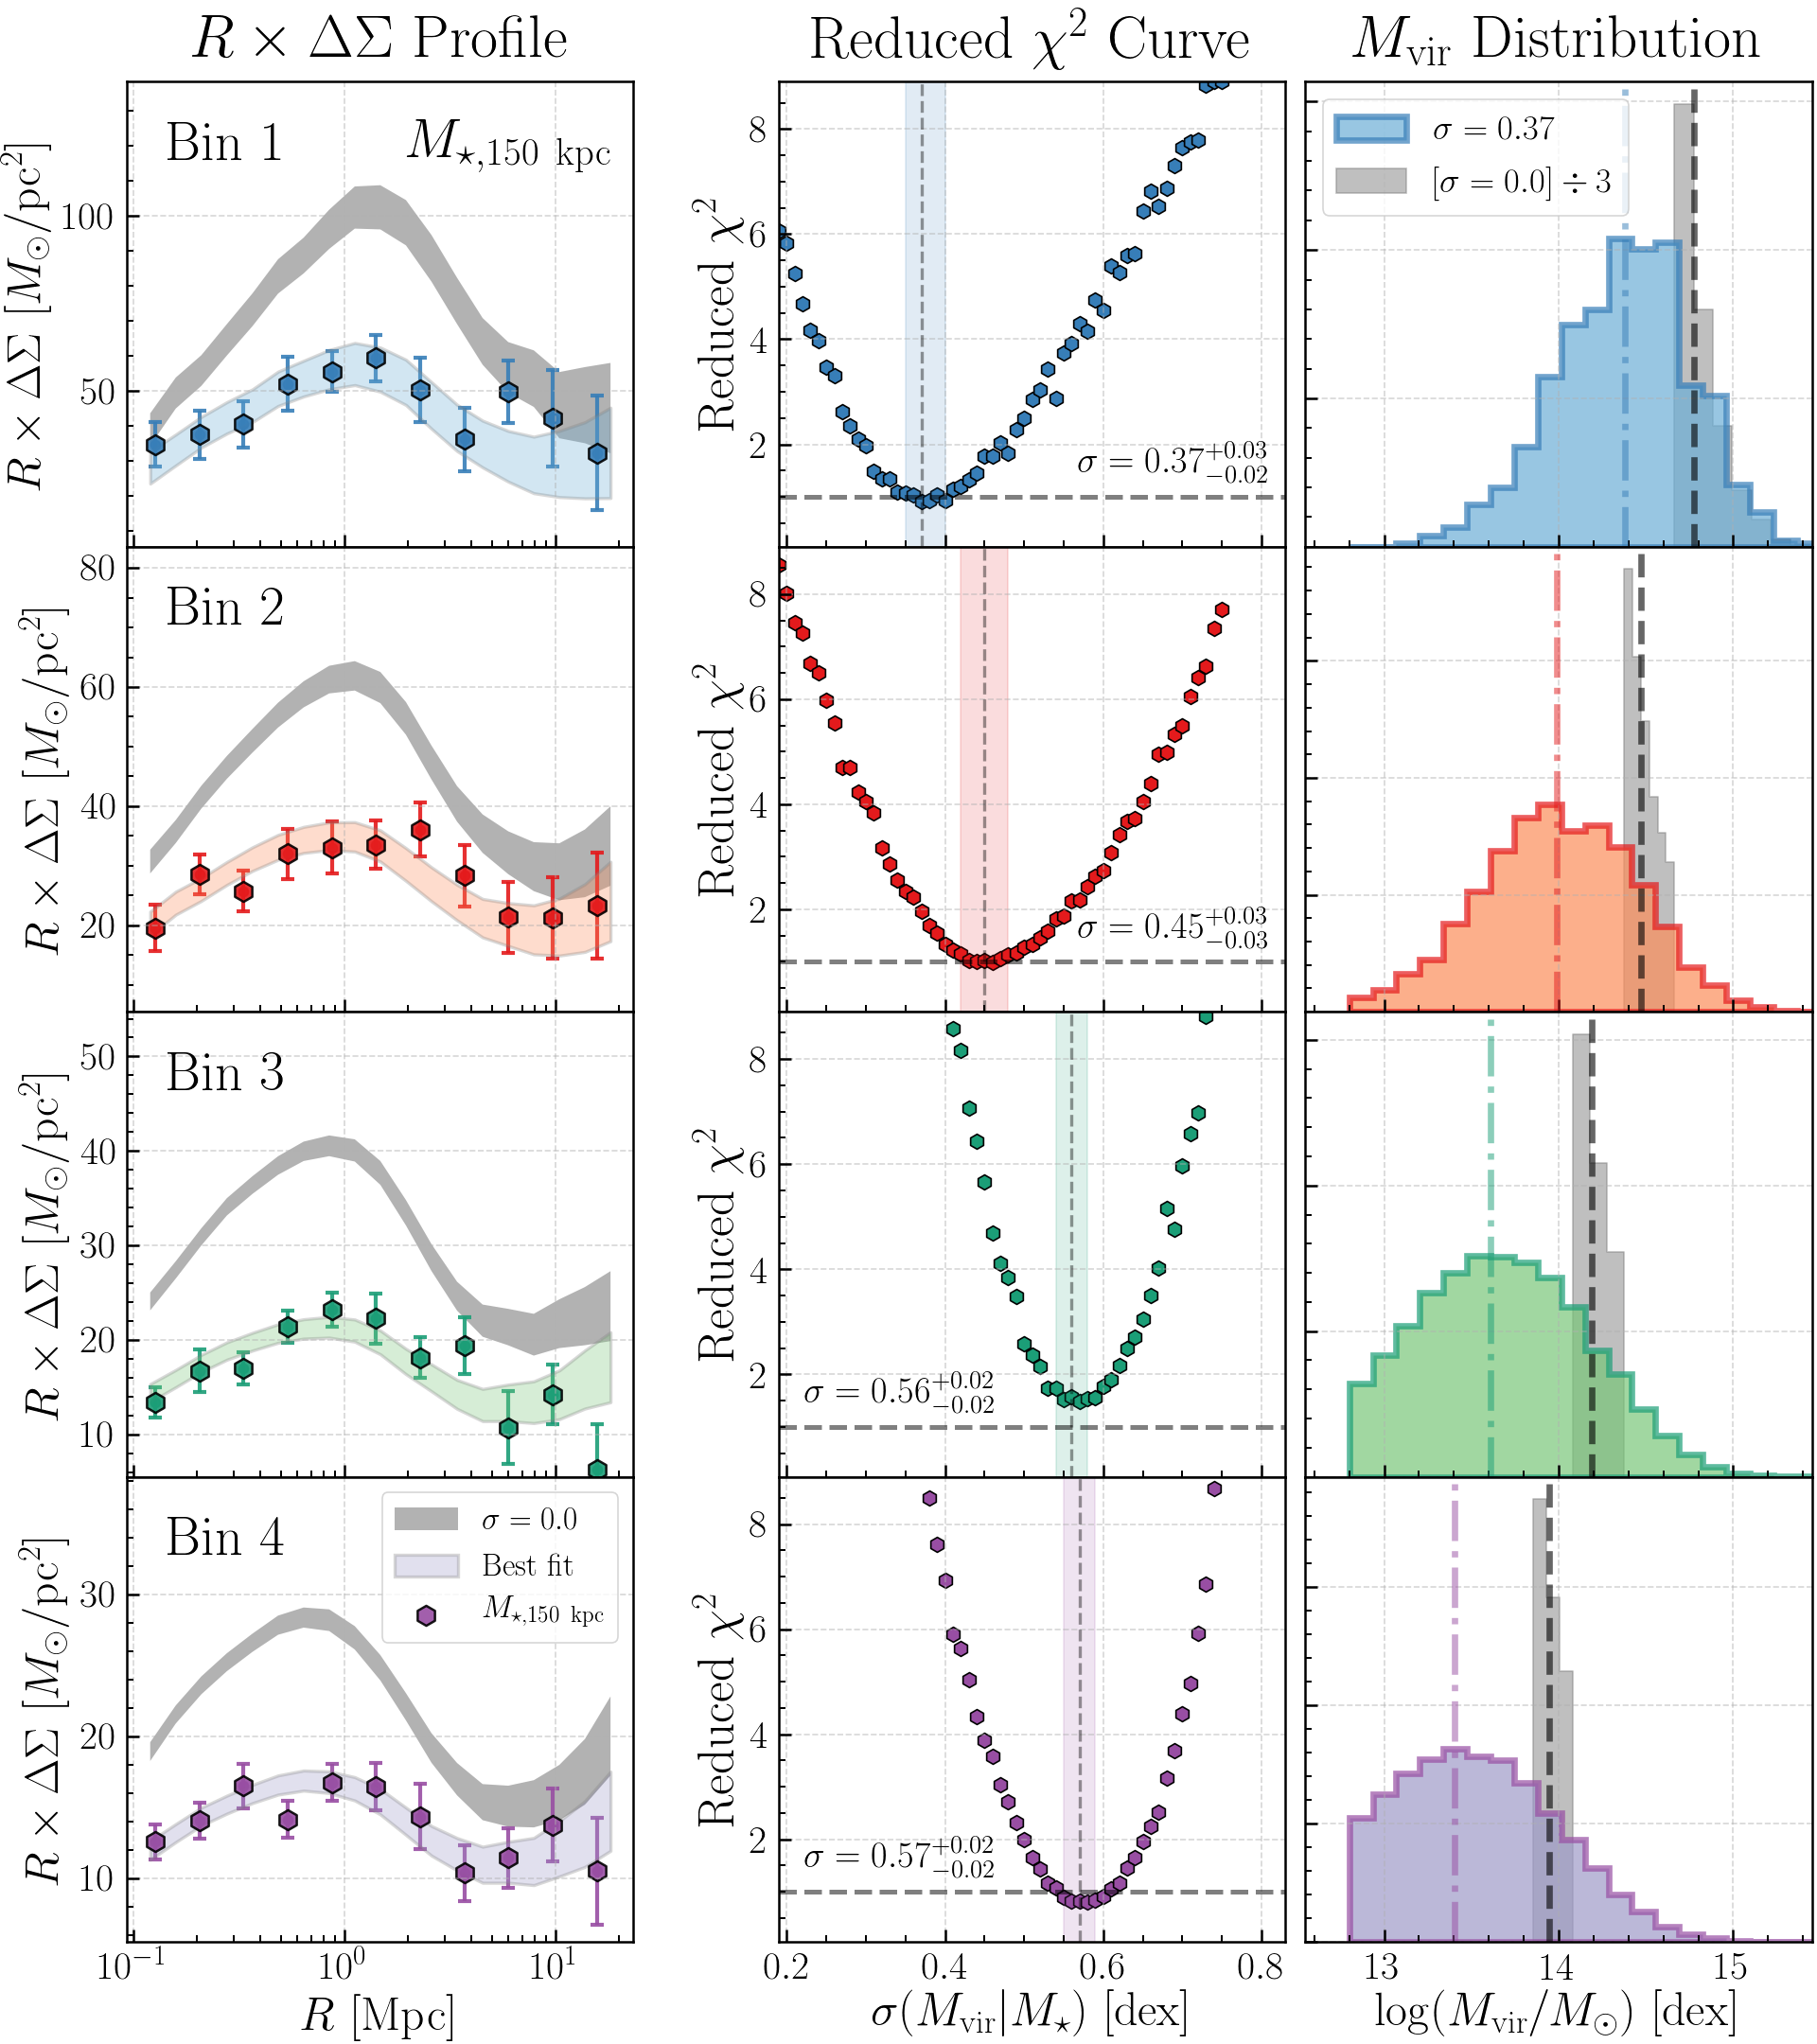
\includegraphics[width=\textwidth]{figure/topn_dsigma_m150_fit}
      \caption{
          \todo{Demonstrate the scatter matching process.}
          }
      \label{fig:fitting}
  \end{figure*}
%% ---------------------------------------------------------------------------------------------- %%
    

%% ---------------------------------------------------------------------------------------------- %%
%% Impact of P_cen on the DSigma profile of richness selected clusters
%% ---------------------------------------------------------------------------------------------- %%
\section{Impact of $P_{\rm cen}$ on the \dsigma{} profile of \redm{} clusters} 
	\label{app:pcen} 
    
    \todo{Placeholder}

%% ---------------------------------------------------------------------------------------------- %%
%% Figure: Impact of Pcen cuts on redMaPPer DSigma profiles.
%% ---------------------------------------------------------------------------------------------- %%
  \begin{figure*}
      \centering 
      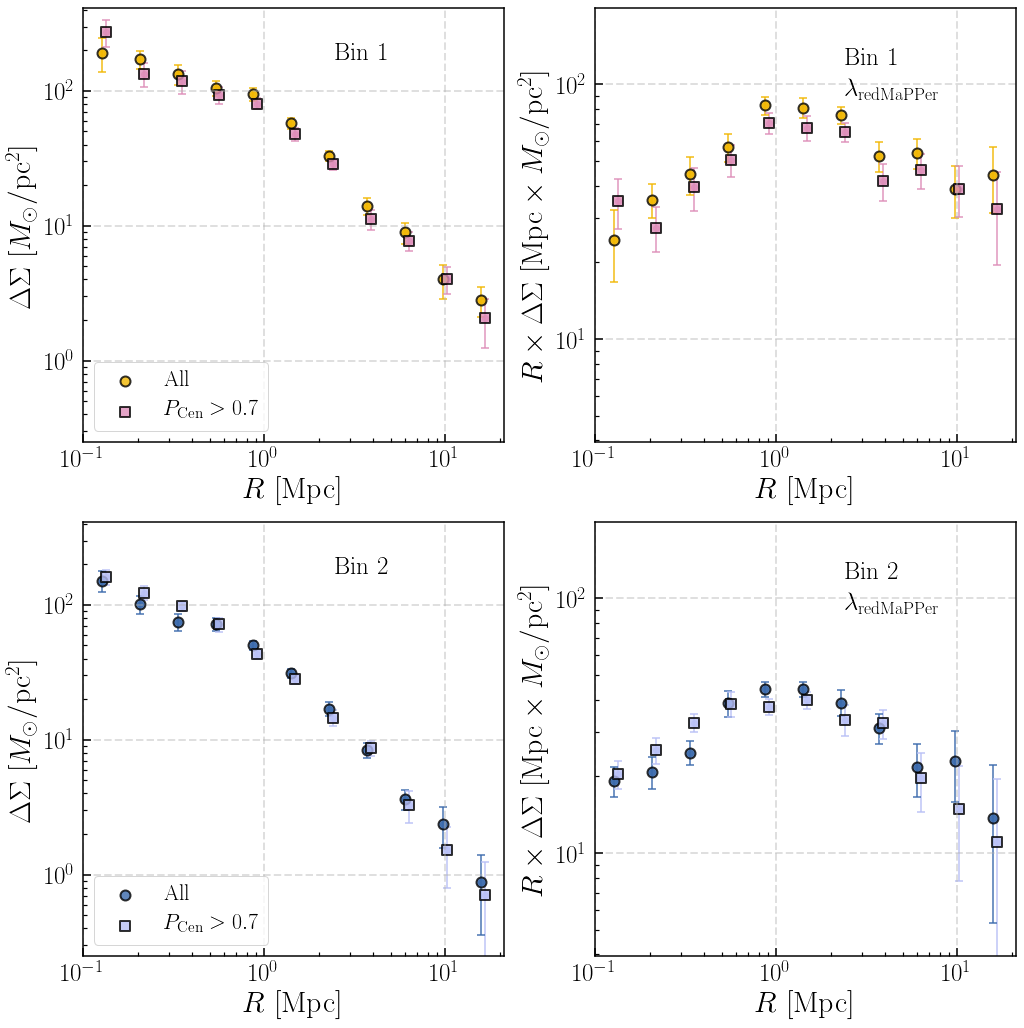
\includegraphics[width=12cm]{figure/redmapper_pcen_placeholder}
      \caption{
          \todo{PLACEHOLDER: Impact of $P_{\rm Cen\ 1}$ cuts on the \redm{} \dsigma{} profiles.
          (For appendix)}
          }
      \label{fig:pcen}
  \end{figure*}
%% ---------------------------------------------------------------------------------------------- %%

%% ---------------------------------------------------------------------------------------------- %%
%% Galaxy size as potential halo mass indicator
%% ---------------------------------------------------------------------------------------------- %%
\section{Galaxy Size as \mvir{} indicator} 
	\label{app:size} 
    
    \todo{Placeholder}


%% ---------------------------------------------------------------------------------------------- %%
\bsp
\label{lastpage}
\end{document}

%% ---------------------------------------------------------------------------------------------- %%
%% ------ End of the File ------
%% ---------------------------------------------------------------------------------------------- %%